\documentclass[12pt,UTF8]{ctexbook}
\usepackage{ctex}
\usepackage{caption}
\usepackage{graphicx}
\usepackage{float}
\usepackage{wrapfig}
\usepackage{array}
\usepackage[table, dvipsnames, svgnames, x11names]{xcolor}
\usepackage{colortbl}% 
\usepackage{tabularx}
\usepackage{amsmath}
\usepackage{amssymb}
\usepackage{xfrac}
\usepackage{eucal}
\usepackage{titlesec}
\usepackage{amsthm}
\usepackage{tikz-cd}
\usepackage{enumitem}
\usepackage{verbatim}
\usepackage{fontspec,xunicode,xltxtra}
\usepackage{xeCJK} 
\usepackage[b]{esvect}

\definecolor{gl}{RGB}{246, 252, 240}
\definecolor{gd}{RGB}{236, 244, 230}
\definecolor{bg}{RGB}{242, 244, 228}


\setCJKmainfont[BoldFont=STZhongsong]{STSong}
\setCJKmonofont{simkai.ttf} % for \texttt
\setCJKsansfont{simfang.ttf} % for \textsf
\setlength\parskip{8pt}
\setlength{\fboxsep}{12pt}
\renewcommand\thesection{\arabic{chapter}.\arabic{section}}
\newtheorem{df}{定义}[section] 
\newtheorem{pp}{命题}[section]
\newtheorem{tm}{定理}[section]
\newtheorem{et}{例题}[section]
\newtheorem{ex}{例子}[section]
\newtheorem{sk}{思考}[section]
\newtheorem{po}{公理}
\newtheorem*{so}{解答}
\newenvironment{proof2}{\paragraph{\textbf{证明:}}}{\hfill$\square$}
\newtheorem{xt}{习题}[section]
\newtheorem{cor}{推论}[pp]
\renewcommand{\proofname}{\indent\bf 证明}
\renewcommand{\qedsymbol}{\hfill$\square$}
% 列举环境的行间距
\setenumerate[1]{itemsep=0pt,partopsep=0pt,parsep=0pt,topsep=0pt}
\setitemize[1]{itemsep=0pt,partopsep=0pt,parsep=0pt,topsep=0pt}
\setdescription{itemsep=0pt,partopsep=0pt,parsep=0pt,topsep=0pt}
\setlength{\intextsep}{2pt}%
\setlength{\columnsep}{2pt}%
% 新函数
\renewcommand\parallel{\mathrel{/\mskip-4mu/}}
% 章节字体大小
\titleformat{\section}{\zihao{-2}\bfseries}{ \thesection }{16pt}{}
% 封面
\title{\zihao{0} \bfseries 第六册}
\author{\zihao{2} \texttt{大青花鱼}}
% \date{\bfseries\today}
\date{}
% 正文
\begin{document}
\maketitle
\tableofcontents
\newpage

\chapter{向量}
第五册中,我们学习了用三角函数解三角形。三角函数是定量研究平面形的利器。
不过,三角函数本身并不是简单的函数。我们目前只能通过查表的方式得到函数值。
这让我们思考,能不能打造一种更方便定量研究的体系呢?

回顾我们对平面形的研究,我们从几条公理出发,得出点、直线、三角形、圆等形状之间的定性关系。
公理体系的缺陷在于没有与数紧密结合。比如,“两点之间直线最短”,除了定性的“最短”,没有提供别的信息。
我们需要一种根本上和数量结合的体系,来理解各种平面形状。

此外,公理体系中并没有强调运动的概念。我们说点运动形成了线,旋转形成角度和圆,
但并没有相关的工具来描述具体的运动。我们需要一种根本上和运动结合的体系,来理解形状之间的关系。

\section{点、向量和直线}
学习有理数的时候,我们使用数轴上的点表示。每个点代表一个实数。两点重合,
当且仅当它们代表同一个数。这种表示方法把数和直线上的点牢牢绑在一起。
我们可以用数的关系表示直线上点的关系。数轴使我们可以定量理解直线。

至于平面中的点,我们用相互垂直的数轴定义了点的坐标。每个点代表一个有序数对。两个数按顺序排列,对应平面中一点。

能不能像数轴一样,用一个量代表平面中一点呢?数轴之所以能用一个数代表一个点,
是因为直线只有两个方向,使用正负号就可以代表方向。平面中不止两个方向,我们无法用正负来表示方向了。
为此,我们引入一个新的量来代表平面中的点:\textbf{向量}。

自然数、有理数、实数都有自己的运算法则。向量作为代表点的量,需要满足怎样的运算法则呢?
我们从运动出发,给出以下的法则:
\begin{enumerate}
    \item 向量的加法就是平移:两个向量相加得到另一个向量。向量的加法满足结合律和交换律。
    \item 零向量表示静止不变:存在这样一个向量,任何向量与它相加,仍然是自己。
    这个向量叫做\textsl{零向量}。零向量不定义方向,也可以说它与任何向量同向或反向。它对应的点称为\textbf{原点}。
    \item 从每个非零向量,引出一根数轴:任何实数乘以向量,得到方向相同或相反的向量。
    这个运算称为\textbf{数乘运算}。数乘运算对应图形的放缩。
    \item 放缩和四则运算相容:数轴上可以做数的运算。
    \item 平移和放缩相容:先平移再放缩,和先放缩再平移,结果一样。
\end{enumerate}
按照定义,\textbf{向量就是点},所以可以用大写字母来表记。比如零向量就是原点,记为$O$。
此外,\textbf{向量就是平移}。点$A$就是把$O$对应到$A$的平移,也是$O$平移的结果,记为$\vv{OA}$。
反过来,$\vv{BA}$就是把$B$对应到$A$的平移。

让我们用数学语言把这些法则更具体地写出来。我们把平面看作集合,记为$\mathbb{V}$,其中的元素称为向量或点,
用粗体小写字母表示,以便和代表数的量区分:
\begin{enumerate}
    \item 加法结合律:$\forall \,\, \mathbf{a}, \mathbf{b}, \mathbf{c} \in \mathbb{V}$,$\mathbf{a}+ (\mathbf{b} + \mathbf{c}) = (\mathbf{a} + \mathbf{b}) + \mathbf{c}$。
    \item 加法交换律:$\forall \,\, \mathbf{a}, \mathbf{b} \in \mathbb{V}$,$\mathbf{a} + \mathbf{b} = \mathbf{b} + \mathbf{a}$。
    \item 存在零向量:$\forall \,\, \mathbf{a} \in \mathbb{V}$,$\mathbf{a} + \mathbf{0} = \mathbf{a}$。
    \item 放缩和四则运算相容:$\forall \,\, \mathbf{a} \in \mathbb{V}$,$1\cdot \mathbf{a} = \mathbf{a}$。$\forall s, t \in \mathbb{R}$,$(s + t)\cdot\mathbf{a} = (s\cdot\mathbf{a}) + (t\cdot\mathbf{a})$,$(s \cdot t)\cdot \mathbf{a} = s \cdot (t\cdot \mathbf{a})$。
    \item 放缩和平移相容:$\forall \,\, \mathbf{a}, \mathbf{b} \in \mathbb{V}$,$\forall \,\, t \in \mathbb{R}$,$t\cdot(\mathbf{a} + \mathbf{b}) = t\cdot\mathbf{a} + t\cdot\mathbf{b}$。
\end{enumerate}

从以上法则出发,我们可以定义直线:
\begin{df}
    过原点的直线是非零向量放缩得到的集合。不过原点的直线是过原点的直线按一点平移得到的集合。
\end{df}
给定非零向量$A = \mathbf{a}$,$ \{t\mathbf{a} \, | \, t\in\mathbb{R}\}$是一条过原点$O$和$A$的直线$OA$,
称为$A$\textbf{引出}的直线,记为$\mathbb{R}\mathbf{a}$。
给定向量$B = \mathbf{b}$,$ \{t\mathbf{a}+\mathbf{b} \, | \, t\in\mathbb{R}\}$是一条过$B$的直线,
记为$\mathbb{R}\mathbf{a}+\mathbf{b}$,其中$\mathbb{R}\mathbf{a}$称为它的线性部分;
而$ \{t\mathbf{a}+(1 - t)\mathbf{b} \, | \, t\in\mathbb{R}\}$就是直线$AB$。

给定非零向量$\mathbf{a}$,如果向量$\mathbf{b}$可以通过$\mathbf{a}$放缩得到,
或者说$\mathbf{b}\in \mathbb{R}\mathbf{a}$,就称两者\textbf{共线}。

类比可以定义线段和射线:给定非零向量$A = \mathbf{a}$和向量$B =\mathbf{b}$,
$ \{(1 - t)\mathbf{a}+t\mathbf{b} \, | \, t\in [0, 1]\}$是线段$AB$,
$ \{(1 - t)\mathbf{a}+t\mathbf{b} \, | \, t \geqslant 0 \}$是射线$AB$。

这样定义的线段和射线,也具备了数轴的性质。比如,在线段$\{t\mathbf{a}+(1 - t)\mathbf{b} \, | \, t\in [0, 1]\}$
中,$t$的不同值就对应了不同的点:$t = 0$对应点$\mathbf{b}$,$t=1$对应点$\mathbf{a}$。对一般的$t\in (0, 1)$,
$t\mathbf{a}+(1 - t)\mathbf{b}$对应的点$P(t)$满足:$|AP(t)| = (1 - t)|AB|$,$|P(t)B| = t|AB|$。也就是说,
$P(t)$是线段$AB$上使得$ \frac{|AP(t)|}{|P(t)B|} = \frac{1 - t}{t}$的点。
$\vv{AP(t)}, \vv{P(t)B}$都和$\vv{AB}$共线。

反过来,设$ \frac{|AP(t)|}{|P(t)B|}$等于定值$k > 0$,对应的点$P(t)$是什么点呢?
这个问题实际上是求方程:
$$ \frac{1 - t}{t} = k$$
的解。容易解出这个方程的唯一解:$t = \frac{1}{k+1}$。因此我们得到结论:
\begin{tm}{\textbf{定比分点定理} }\label{tm:0-0-10}
    线段$AB$上到两端距离之比$\frac{|AP|}{|PB|}$为定值$k$的点$P$恰有一个,称为它的$k$\textbf{分点}。
\end{tm}
正数$k$越小,$k$分点距离$A$越近,$k$越大,$k$分点离$A$越远;$k=1$时,我们就得到线段的中点。

以上我们讨论了$k>0$的情况,显然,$k=0$对应$P = A$。对于负数$k$,有没有对应的点呢?
我们用平移的思想考虑这个问题,从$A$到$P(t)$经历的平移是$\vv{AP(t)} = (1 - t)\vv{AB}$,
从$P(t)$到$B$经历的平移是$\vv{P(t)B} = t\vv{AB}$。它们的系数之比就是$ \frac{1 - t}{t}$。
于是,我们可以对一般的$k$定义定比分点:如果$k$能使得方程
$$ \frac{1 - t}{t} = k$$
有唯一解,那么我们就把对应的点$P(t)$称为$AB$的$k$分点。

如果$k<-1$,那么$k$分点对应的$t = \frac{1}{k+1} < 0$,也就是说,$P(t)$在线段$BA$沿$B$的延长线上。
如果$-1<k<0$,那么$k$分点对应的$t = \frac{1}{k+1} > 1$,也就是说,$P(t)$在线段$BA$沿$A$的延长线上。
如果$k=-1$,以上方程无解,这说明$-1$分点不存在。

共线的向量,通过数轴,可以方便地讨论相互的位置关系。不共线的向量之间,
如何讨论位置关系呢?为此,我们要引入\textbf{平面的根本性质}:
\begin{enumerate}
    \item 给定任何非零向量$A$,平面中总有另一个向量$B$,不在直线$OA$上。我们说两者\textbf{不共线}。
    \item 从不共线的向量$A, B$出发,经过放缩、平移,可以得到平面中任何向量。具体来说,
    任何向量都可以表示成$sA + tB$的形式,集合$\{sA + tB \,|\, s, t, \in\mathbb{R}\}$就是整个平面。
    这样的$A, B$称为平面的一组\textbf{基}或\textbf{基底}。
\end{enumerate}

举例来说,在直角坐标系中,我们选择了原点重合、互相垂直的两条数轴,
以每条数轴上数$1$对应的点(记为$\mathbf{e}_x, \mathbf{e}_y$)出发,通过放缩和平移,
就得到平面所有的点。平面中任一点可以写成$x\mathbf{e}_x + y\mathbf{e}_y$,其中$x,y$就是点的坐标。
直角坐标系其实是一种用向量描述平面的方法。$\mathbf{e}_x, \mathbf{e}_y$就是一组基。

\begin{sk}\label{sk:0-0-10}
    \mbox{}\\
    1. 设平面上有两点$A,B$,以$OA, OB$为邻边作平行四边形$AOBC$。向量$\vv{OA}$和$\vv{BC}$是什么关系?\\
    2. 设平面上有两点$A,B$,三角形$OAB$中,连接边$OA, OB$的中点$M,N$。向量$\vv{AB}$和$\vv{MN}$是什么关系?
\end{sk}
\begin{xt}\label{xt:0-0-10}
    \mbox{} \\
    \indent 1. 证明:零向量只有一个,任何向量乘$0$得到零向量。\\
    \indent 2. 证明:零向量乘任何数得到零向量。\\
    \indent 3. 证明:任何向量$\mathbf{a}$都有唯一的反向量$\mathbf{b}$,满足$\mathbf{a} + \mathbf{b} = \mathbf{0}$。\\
    \indent 4. 设$\mathbf{a}, \mathbf{b}$不共线,如果$s\mathbf{a} + t\mathbf{b} = \mathbf{0}$,证明:$s = t = 0$。\\
    直角坐标系$xOy$中,设$\mathbf{a} = 4\mathbf{e}_x + \mathbf{e}_y$,$\mathbf{b} = \mathbf{e}_x - 2\mathbf{e}_y$
    ,$\mathbf{b} = -\mathbf{e}_x + 2\mathbf{e}_y$。\\
    \indent 5. 在坐标轴上标出$\mathbf{a}$,$\mathbf{b}$和$\mathbf{c}$。\\
    \indent 6. 用$\mathbf{a}$和$\mathbf{b}$表示$\mathbf{e}_x$、$\mathbf{e}_y$和点$(3,0)$。\\
    \indent 7. 用$\mathbf{a}$和$\mathbf{b}$表示它们的中点、$3$分点、$-0.5$分点、$-3$分点。
    写出这些点的坐标和直线的方程。\\
    \indent 8. 用$\mathbf{a}, \mathbf{b}, \mathbf{c}$表示顶点为$\mathbf{a}, \mathbf{b}, \mathbf{c}$的三角形三边和重心。
\end{xt}

\section{角度与长度}
根据平面的根本性质,任何向量都可以用两个不共线向量表示。如何讨论它们的位置关系呢?
下面我们定义一种关系,把长度、距离和角度统一起来。

给定平面基底$\mathbf{e}_1, \mathbf{e}_2$,我们给出这样一个二元映射$f$:
$$ \forall \,\, \mathbf{a} = x_A\mathbf{e}_1 + y_A\mathbf{e}_2, \,\, \mathbf{b} = x_B\mathbf{e}_1 + y_B\mathbf{e}_2, \,\, \in \mathbb{R}, \quad f(\mathbf{a}, \mathbf{b}) = x_Ax_B + y_Ay_B.$$
$f$把两个向量对应到一个实数。它满足以下五个性质:
\begin{enumerate}
    \item 向量的顺序不影响关系大小:
    \begin{align}
         & f(x_A\mathbf{e}_1 + y_A\mathbf{e}_2, x_B\mathbf{e}_1 + y_B\mathbf{e}_2) \notag \\
        =\,\,& x_Ax_B + y_A y_B = x_Bx_A + y_By_A \notag \\
        =\,\,& f(x_B\mathbf{e}_1 + y_B\mathbf{e}_2, x_A\mathbf{e}_1 + y_A\mathbf{e}_2). \notag
    \end{align}
    \item 零向量和任意向量关系为$0$:
    $$f(x_A\mathbf{e}_1 + y_A\mathbf{e}_2, \mathbf{0}) = f(x_A\mathbf{e}_1 + y_A\mathbf{e}_2, 0\mathbf{e}_1 + 0\mathbf{e}_2) = x_A\cdot 0 + y_A\cdot 0 = 0.$$
    \item 非零向量与自身的关系总是正的:$x_A, y_A$不全为零时,
    $$f(x_A\mathbf{e}_1 + y_A\mathbf{e}_2, x_A\mathbf{e}_1 + y_A\mathbf{e}_2) = x_A^2 + y_A^2  > 0.$$
    \item 和向量的放缩相容:
    \begin{align}
        & f(x_A\mathbf{e}_1 + y_A\mathbf{e}_2, t(x_B\mathbf{e}_1 + y_B\mathbf{e}_2)) \notag \\
        =\,\,& x_Atx_B + y_A ty_B = t(x_Ax_B + y_Ay_B) \notag \\
        =\,\,& tf(x_A\mathbf{e}_1 + y_A\mathbf{e}_2, x_B\mathbf{e}_1 + y_B\mathbf{e}_2). \notag 
    \end{align}
    \item 和向量的平移相容:
    \begin{align}
         & f(x_A\mathbf{e}_1 + y_A\mathbf{e}_2, (x_B\mathbf{e}_1 + y_B\mathbf{e}_2) + (x_C\mathbf{e}_1 + y_C\mathbf{e}_2)) \notag \\
         =\,\,& x_A(x_B + x_C) + y_A (y_B + y_C) = (x_Ax_B + y_Ay_B) + (x_Ax_C + y_Ay_C) \notag \\
         =\,\,& f(x_A\mathbf{e}_1 + y_A\mathbf{e}_2, x_B\mathbf{e}_1 + y_B\mathbf{e}_2) + f(x_A\mathbf{e}_1 + y_A\mathbf{e}_2, x_C\mathbf{e}_1 + y_C\mathbf{e}_2). \notag
    \end{align}     
\end{enumerate}
满足以上五个条件的映射$f$称为平面向量的\textbf{内积}。从第四个性质可知,向量与自身的内积总是正数。
我们把这个数的平方根叫做\textbf{向量的长度},记为:
$$ \forall \,\, \mathbf{a} \in \mathbb{V}, \quad \| \mathbf{a}\| = \sqrt{f(\mathbf{a}, \mathbf{a})}. $$
两个向量之差的长度,称为向量之间的距离。
$$ \forall \,\, \mathbf{a}, \mathbf{b} \in \mathbb{V}, \quad \| \mathbf{a} - \mathbf{b}\| = \sqrt{f(\mathbf{a} - \mathbf{b}, \mathbf{a} - \mathbf{b})}. $$
如果基底$\mathbf{e}_1, \mathbf{e}_2$是直角坐标系的基,那么
\begin{align}
    \forall \,\, \mathbf{a} = x_A\mathbf{e}_x &+ y_A\mathbf{e}_y , \notag \\
    \| \mathbf{a}\| &= \sqrt{x_A^2 + y_A^2}, \notag \\
    \forall \,\, \mathbf{a} = x_A\mathbf{e}_x &+ y_A\mathbf{e}_y,\,\,\, \mathbf{b} = x_B\mathbf{e}_x + y_B\mathbf{e}_y , \notag \\
    \| \mathbf{a} - \mathbf{b}\| &= \sqrt{(x_A - x_B)^2 + (y_A - y_B)^2}. \notag
\end{align}
给定向量$A = \mathbf{a}$、$B =\mathbf{b}$,$\| \mathbf{a} \|$就是$|OA|$,
$\|\mathbf{a} - \mathbf{b}\|$就是$|AB|$。
也就是说,通过内积定义的映射$f$,分别与直观经验中长度和距离的概念相符合。

那么,$f$本身有什么含义呢?我们来计算$ \frac{|OA|^2 + |OB|^2 - |AB|^2}{2}.$
\begin{align}
    \frac{|OA|^2 + |OB|^2 - |AB|^2}{2} &= \frac{x_A^2 + y_A^2 + x_B^2 + y_B^2 - (x_A - x_B)^2 - (y_A - y_B)^2}{2} \notag \\
    &= x_Ax_B + y_Ay_B = f(\mathbf{a}, \mathbf{b}). \notag 
\end{align}
另一方面,余弦定理告诉我们,$ \frac{|OA|^2 + |OB|^2 - |AB|^2}{2} = |OA||OB|\cos \angle AOB$。
也就是说,$f(\mathbf{a}, \mathbf{b}) = \|\mathbf{a}\| \|\mathbf{b}\| \cos \angle AOB$。% \langle \mathbf{a}, \mathbf{b}\rangle 
内积$f$的本质是向量夹角的余弦与向量长度的乘积。通过内积,我们把角度和长度统一起来了。

向量夹角的余弦值总在$-1$和$1$之间,所以向量的内积的绝对值不大于向量长度的乘积:
$$ |x_Ax_B + y_Ay_B| \leqslant \sqrt{x_A^2 + y_A^2} \sqrt{x_B^2 + y_B^2}.$$
可以验证这个关系对任意$x_A, y_A, x_B, y_B$成立。从这个关系出发,可以得到:
$$ |AB| = \sqrt{(x_A - x_B)^2 + (y_A - y_B)^2} \leqslant \sqrt{x_A^2 + y_A^2} + \sqrt{x_B^2 + y_B^2} = |OA| + |OB|.$$
这符合直观经验中“三角形两边之和大于第三边”或“两点之间线段距离最短”的性质。

内积为$0$,就表示向量夹角的余弦为$0$,即两个向量垂直。
比如令$\mathbf{a} = 2\mathbf{e}_x - \mathbf{e}_y$,$\mathbf{b} = \mathbf{e}_x + 2\mathbf{e}_y$,
那么$f(\mathbf{a}, \mathbf{b}) = 2\cdot 1 - 1\cdot 2 = 0$。在平面上画出对应的点$A,B$,
可以验证$\angle AOB = 90^\circ$。

内积映射并不是唯一的,我们看另一个映射$f_2$:
$$ \forall \,\, x_A, y_A, x_B, y_B \in \mathbb{R}, \quad f(x_A\mathbf{e}_1 + y_A\mathbf{e}_2, x_B\mathbf{e}_1 + y_B\mathbf{e}_2) = 2x_Ax_B + y_A y_B.$$
可以验证,$f_2$也满足$f$满足的五个性质。从$f_2$出发,我们也可以定义距离和长度:
$$ \forall \,\, \mathbf{a} = x_A\mathbf{e}_x + y_A\mathbf{e}_y, \quad \| \mathbf{a} \|_2 = f_2(\mathbf{a}, \mathbf{a}) = 2x_A^2 + y_A^2. $$
这样定义的距离和长度和我们直观经验中有些不一样,不过,我们可以验证,这样定义的距离也满足“两点之间线段最短”的性质。
$$ |2x_Ax_B + y_Ay_B| \leqslant \sqrt{2x_A^2 + y_A^2} \sqrt{2x_A^2 + y_A^2}.$$
因此,$f_2$也是内积。

我们把符合直观经验的内积$f$称为\textbf{经典内积},一般称内积都默认指经典内积;
把对应的长度称为向量的\textbf{模}。
我们把$\mathbf{a}, \mathbf{b}$的(经典)内积记为$(\mathbf{a}\, | \, \mathbf{b})$,
不至于混淆时,也常称为\textbf{点积},记为$\mathbf{a} \cdot \mathbf{b}$;
把它们的模记为$|\mathbf{a}|$、$|\mathbf{b}|$。

既然有余弦,自然有正弦。记$\alpha = \angle AOB$,
则$(\mathbf{a}\, | \, \mathbf{b}) = |\mathbf{a}||\mathbf{b}| \cos \alpha$,
于是,
$$ |\mathbf{a}|^2|\mathbf{b}|^2 \sin^2 \alpha = |\mathbf{a}|^2|\mathbf{b}|^2 - (\mathbf{a}\, | \, \mathbf{b})^2 $$
记$\mathbf{a} = x_A\mathbf{e}_x + y_A\mathbf{e}_y$,$\mathbf{b} = x_B\mathbf{e}_x + y_B\mathbf{e}_y$,
则
\begin{align}
    (x_A^2 + y_A^2)(x_B^2 + y_B^2) \sin^2 \alpha &= (x_A^2 + y_A^2)(x_B^2 + y_B^2) - (x_Ax_B + y_Ay_B)^2 \notag \\
    &= (x_Ay_B - x_By_A)^2 \notag \\
    |\sin \alpha| &= \frac{|x_Ay_B - x_By_A|}{\sqrt{x_A^2 + y_A^2} \sqrt{x_B^2 + y_B^2}} \notag
\end{align}
我们得出了夹角$\angle AOB$正弦的绝对值。

观察向量夹角的正弦和余弦,我们注意到,它们的表达式与和差角公式有相似之处。
$x_Ax_B + y_Ay_B$与差角余弦公式形式相似,$x_Ay_B - x_By_A$与差角正弦公式形式相似。

让我们在直角坐标系中找几个例子,看看直观结果。设有点$A(1,\,\,0)$、$B(\frac{1}{2},\frac{\sqrt{3}}{2})$。
不难得出$\angle AOB = 60^\circ$。我们用以上公式计算$\angle AOB$的正弦和余弦:
$$ \frac{x_Ay_B - x_By_A}{\sqrt{x_A^2 + y_A^2}\sqrt{x_B^2 + y_B^2}} = \frac{\sqrt{3}}{2}, \quad \frac{x_Ax_B + y_Ay_B}{\sqrt{x_A^2 + y_A^2} \sqrt{x_B^2 + y_B^2}} = \frac{1}{2}. $$
把$P$的坐标换成$(0,\,\,1)$、$(-\frac{\sqrt{2}}{2}, \frac{\sqrt{2}}{2})$、$(\frac{\sqrt{3}}{2},-\frac{1}{2})$等,
我们发现,通过以上两个公式得到的值,分别是$\angle AOB$的正弦、余弦值。
记$\angle AOB = \alpha$,那么:
$$ \sin \alpha = \frac{x_Ay_B - x_By_A}{\sqrt{x_A^2 + y_A^2}\sqrt{x_B^2 + y_B^2}}, \quad \cos \alpha = \frac{x_Ax_B + y_Ay_B}{\sqrt{x_A^2 + y_A^2} \sqrt{x_B^2 + y_B^2}}. $$

% 要注意的是,以上公式成立,是因为直角坐标系$xOy$的$x$轴和$y$轴沿逆时针顺序摆放,同时规定逆时针方向为角度的正方向。
% 如果直角坐标系的坐标轴摆放顺序和角度的正方向相反,以上的公式就要改为:
% $$ \sin \alpha = \frac{x_By_A - x_Ay_B}{\sqrt{x_A^2 + y_A^2}\sqrt{x_B^2 + y_B^2}}, \quad \cos \alpha = \frac{x_Ax_B + y_Ay_B}{\sqrt{x_A^2 + y_A^2} \sqrt{x_B^2 + y_B^2}}. $$

我们是通过面积定义正弦的。比如,邻边为$OA$和$OB$的平行四边形,面积是$|OA||OB|\sin \angle AOB$。
对照上面正弦的表达式,可以发现这个面积等于$x_Ay_B - x_By_A$。于是,我们把对应的映射
$$ (\mathbf{a}, \,\,\mathbf{b}) \mapsto x_Ay_B - x_By_A. $$
称为向量$A, B$的\textbf{面积},记为$\mathbf{a} \wedge \mathbf{b}$。

向量的面积和内积,分别对应正弦和余弦。两向量面积为零,当且仅当它们共线;两向量内积为零,当且仅当它们互相垂直。

\begin{xt}
    \mbox{} \\
    1. 直角坐标系中,已知两向量,计算它们的内积和面积,讨论它们的关系。\\
    \indent 1.1. $A(0,\,\, 2), \,\,\, B(1, \,\,1)$ \\
    \indent 1.2. $A(2,\,\, 1),\,\,\,  B(0.5, \,\,-1)$ \\
    \indent 1.3. $A(1.6,\,\, 0.2), \,\,\, B(-0.9,\,\, -3)$\\
    \indent 1.4. $A(1, \,\,-0.28), \,\,\, B(-0.45,\,\, -0.6)$\\
    2. 直角坐标系中,已知向量$B$的模为$2$,根据以下条件,求向量$A,B$的内积:\\
    \indent 2.1 $A = (-4, \,\,2), \,\,\, \angle AOB = 60^\circ$\\
    \indent 2.2 $A= (0,\,\, 5), \,\,\,\angle AOB = 135^\circ$\\
    \indent 2.3.$A = (3,\,\, -2.5), \,\,\,\angle AOB = 45^\circ$\\
    3. 直角坐标系中,已知点$P(2,\,\,1)$,求使得$P,Q$内积为$4$的点$Q$。\\
    4. 直角坐标系中,已知点$P(2,\,\,1)$,求使得$P,Q$面积为$4$的点$Q$。
\end{xt}

\begin{sk}
    如果直角坐标系$xOy$的$x$轴和$y$轴沿逆时针排布,而角度的正方向为顺时针方向,角$\alpha$的正弦和余弦是否还能写成
    $$ \sin \alpha = \frac{x_Ay_B - x_By_A}{\sqrt{x_A^2 + y_A^2}\sqrt{x_B^2 + y_B^2}}, \quad \cos \alpha = \frac{x_Ax_B + y_Ay_B}{\sqrt{x_A^2 + y_A^2} \sqrt{x_B^2 + y_B^2}}$$
    的形式?
\end{sk}

\section{直线的方程}
我们已经讨论过直线和方程的关系。
直角坐标系中,任意给定二元一次方程$ax + by + c = 0$($a$、$b$不全为$0$),
它的解集都对应平面中一条直线。我们把这个二元一次方程称为直线的\textbf{一般式}方程。
比如,$3x - 2y + 1 = 0$就是一条直线的一般式方程。不过,从这个式子,我们不容易看出相应的直线有什么性质。
已知直线的一些直观性质,我们希望将这些直观性质和直线的方程联系起来,
以便通过方程的方式,来分析直线以及直线和其他平面形的关系。

比如,已知直线过点$A(x_A,\,\, y_A)$,斜率为$k$。
直线斜率为$k$,说明直线是某个一次函数$x \mapsto kx + b$的图像。
对比可知,直线方程为:
$$y - y_A = k(x - x_A).$$
我们把这个方程称为直线的\textbf{点斜式}方程。已知直线上一点和直线的斜率,可以写出直线的点斜式方程。
比如,过$(1,\,\,2)$,斜率为$2$的直线方程为:$y - 2 = 2(x - 1)$,即$y - 2x = 0$。

下面我们用向量的语言,给出有不同直观性质的直线的方程。

\textbf{点向式}:已知直线过点$A(x_A,\,\, y_A)$,方向向量为$\mathbf{b} = (x_B,\,\, y_B)$,
那么直线为$A + \mathbb{R}\mathbf{b}$。
考虑直线上一点$P(x,\,\, y)$,$\vv{AP}$和$\mathbf{b}$共线,所以面积为$0$。
于是$(x,\,\,y)$满足方程:
$$(x - x_A) y_B - (y - y_A) x_B = 0.$$
我们把这个二元一次方程称为直线的点向式方程。已知直线上一点和直线的方向,可以写出直线的点向式方程。
比如,过$(1,\,\,2)$,方向为$(-1,\,\,1)$的直线方程为:$1\cdot(x - 1) - (-1)\cdot(y - 2) = 0$,即$x + y = 3$。

\textbf{两点式}:已知直线过点$A(x_A,\,\, y_A)$和点$B(x_B,\,\, y_B)$,那么直线为$A + \mathbb{R}\vv{AB}$。
考虑直线上一点$P(x,\,\, y)$,则$\vv{AP}$和$\vv{AB}$共线。
于是$(x,\,\,y)$满足方程:
$$(x - x_A) (y_B - y_A) - (y - y_A) (x_B - x_A) = 0.$$
我们把以上方程称为直线的两点式方程。已知直线上不同的两点,可以写出直线的两点式方程。比如,
过$(1,\,\,2)$、$(-2,\,\,1)$的直线方程为:$(x - 1)(1 - 2) - (y - 2)(-2 - 1) = 0$,即$-x + 3y = 5$。

\textbf{点法式}:已知直线过点$A(x_A,\,\, y_A) = \mathbf{a}$,并且和$\mathbf{b} = (x_B,\,\, y_B)$垂直。
考虑直线上一点$P(x,\,\, y) = \mathbf{p}$,$\mathbf{p} - \mathbf{a}$和$\mathbf{b}$垂直,所以内积为$0$。
于是$(x,\,\,y)$满足方程:
$$(x - x_A) x_B + (y - y_A) y_B = 0.$$
我们把$\mathbf{b}$称为直线的\textbf{法向量},把以上方程称为直线的点法式方程。已知直线上一点和法向量,
可以写出直线的点法式方程。比如,过$(1,\,\,2)$,法向量为$(3,\,\,-1)$的直线方程为:
$(x - 1)\cdot 3 + (y - 2)\cdot (-1) = 0$,即$3x - y= 1$。

\textbf{等高式}:已知点$P(x,\,\, y) = \mathbf{p}$与$B(x_B,\,\, y_B) = \mathbf{b}$的面积为$S$,
则$(x,\,\,y)$满足方程:
$$x y_B - y x_B = S.$$
我们把这个二元一次方程称为直线的等高式方程。从直观上看,它表示所有以$OB$为底,
面积相等(从而高相等)的三角形$OBP$的顶点$P$的集合,即一条平行于$OB$的直线。
比如,与$(1,\,\,-1)$的面积为$3$的点构成直线,方程为:$-x + y = 3$。

$S=0$时,我们就得到直线$OB$。也就是说,已知$B$的坐标$(x_B,\,\, y_B)$,直线$OB$的方程是$x y_B - y x_B = 0$。

\textbf{等垂式}:已知点$P(x, \,\,y) = \mathbf{p}$与$B(x_B, \,\,y_B) = \mathbf{b}$的内积为$T$,
则$(x,\,\,y)$满足方程:
$$x x_B + y y_B = T.$$
我们把这个二元一次方程称为直线的等垂式方程。

从直观上看,作$P$到直线$OB$的垂线,垂足为$H$。设$\vv{OH} = t \vv{OB}$,
$$ T = \vv{OP} \cdot \vv{OB} = \vv{OH} \cdot \vv{OB} + \vv{HP} \cdot \vv{OB}.$$
$ HP \perp OB$,所以$\vv{HP} \cdot \vv{OB} = 0$。于是$T = t \vv{OB} \cdot \vv{OB} = t|OB|^2$,
算得$t = \frac{T}{|OB|^2}$,$\vv{OH} = \frac{T}{|OB|^2} \vv{OB}$。这说明$H$是定点。

反之,过$H$点作垂直$OB$的直线。直线上任一点到$OB$的垂足是$H$,因此$\vv{OP} \cdot \vv{OB} = T$。

这说明直线$x x_B + y y_B = T$是一条垂直于$OB$的直线,是所有到$OB$的垂足为定点$H$的点$P$的集合。
比如,与点$B(1,\,\,-1)$的内积为$3$的点构成直线,方程为:$x - y = 3$。它垂直于直线$OB$:$x + y = 0$。

使用等高式和等垂式,我们可以讨论直线平行和垂直的关系。我们来看两个典型问题:

\begin{ex}
    求经过点$P(x_P, \,\,y_P)$并平行于直线$l: \,\, ax + by + c = 0$的直线(如果存在)的方程。
\end{ex}
\begin{so}
首先把直线方程转为等高式:$ax - (-b)y = -c$,它表示平行于向量$(a, -b)$,与它的面积为$-c$的直线。
如果$P$在直线上,那么$P$满足$ax_P - (-b)y_P = -c$。这时符合要求的平行线不存在。
如果$P$不在直线上,我们可以构造直线$l' : \,\, ax - (-b)y = ax_P - (-b)y_P$。$l'$过$P$,且与向量$(a, -b)$平行,
因此平行于$l$。

另一方面,如果有直线过点$P$并平行于$l$,那么它与向量$(a, -b)$平行。设它的方程为
$ax - (-b)y = S$。由于$P$在直线$ax - (-b)y = S$上,$P$满足$ax_P - (-b)y_P = S$,即平行线方程为
$ax - (-b)y = ax_P - (-b)y_P$。显然,$ax_P - (-b)y_P = -c$时,两直线重合,不符合平行线定义。

因此,$ax_P - (-b)y_P = -c$($P$在直线上)时无平行线;其他情况下,恰有一条平行线:$ax - (-b)y = ax_P - (-b)y_P$。
化简后的方程为:$ax + by = ax_P + y_P$。

\textbf{另解:}首先把直线方程转为等垂式:$ax + by = -c$,它表示与点$M(a, b)$的内积为$-c$的直线,
也就是垂直于$OM$,垂足$Q$满足$\vv{OQ} = \frac{-c}{|OM|^2}\vv{OM}$的直线。
如果有直线过点$P$并平行于$l$,那么它也和$OM$垂直。把它写成等垂式:$ax + by = T$。由于$P$在$l'$上,
所以$T = ax_P + y_P$。于是$l'$的方程为$ax + by = ax_P + y_P$。显然,$ax_P + by_P = -c$时,两直线重合,不符合平行线定义。

另一方面,考察$l' : \,\, ax + by = ax_P + y_P$,它垂直于$OM$,所以与$l$平行或重合。容易验证,两线重合当且仅当$ax_P + by_P = -c$。

因此,$ax_P + by_P = -c$($P$在直线上)时无平行线;其他情况下,恰有一条平行线:$ax + by = ax_P + y_P$。

我们发现,与$ax + by + c = 0$平行的直线,总可以写成$ax + by + c' = 0$的形式。我们把$ax + by$称为直线的头。
头相同的直线相互平行或重合。
\end{so}

\begin{et}
    求经过点$P(x_P, \,\,y_P)$并垂直于直线$l: \,\, ax + by + c = 0$的直线(如果存在)的方程。
\end{et}
\begin{so}
    把直线方程写成点法式:$(x - x_Q)a + (y - y_Q)b = 0$,其中$Q(x_Q, y_Q)$是$l$上一点。
这说明$(a, b)$是$l$的法向量。因此,以$(a, b)$为方向的直线:$(x - x_P)b - (y - y_P)a = 0$就是过$P$且垂直于$l$的直线。
\end{so}

我们发现,与$ax + by + c = 0$垂直的直线,总可以写成$bx - ay + c' = 0$的形式。

\begin{et}
    给定一点$P(x_P, \,\,y_P)$和一条直线$l: \,\, ax + by + c = 0$,如何计算$P$到直线$l$的距离$d$?
\end{et}
\begin{so}
    首先把直线方程转为等高式:$ax - (-b)y = -c$,它表示与点$M(a, -b)$的面积为$-c$的直线。
$P$与点$M$的面积为$ax_P - (-b)y_P$。如果$P$到$l$的垂足为$Q$,
$P$到$OM$的垂足为$H$,那么$P$到$l$的距离$d = |PQ|$是$|HQ|$与$|PH|$的差。
平行四边形的面积等于底乘以高,所以,考虑$P$、$Q$分别与$O, M$生成的平行四边形,
它们的面积之差等于高的差乘以底。而两者对应的高分别是$|HQ|$与$|PH|$。
也就是说,$P$到$l$的距离$d$是两个面积的差除以底的商:
$$ d = \frac{|-c - (ax_P - (-b)y_P)|}{\sqrt{a^2 + (-b)^2}} = \frac{|ax_P + by_P + c|}{\sqrt{a^2 + b^2}}.$$

\textbf{另解:}首先把直线方程转为等垂式:$ax + by = -c$,它表示与点$M(a, b)$的内积为$-c$的直线,
也就是垂直于$OM$,垂足$Q$满足$\vv{OQ} = \frac{-c}{|OM|^2}\vv{OM}$的直线。作$P$到$OM$的垂线$l'$,记垂足为$H$,则$P$到$l$的距离就是$|HQ|$,
也就是$|OQ|$和$|OH|$的差。$l$与$l'$垂直于同一条直线$OM$,因此平行或重合。于是$l'$的等垂式为$ax + by = ax_P + by_P$,
$\vv{OH} = \frac{T}{|OM|^2}\vv{OM} = \frac{ax_P + by_P}{|OM|^2}\vv{OM}$。于是$P$到$l$的距离为:
$$ d = |\vv{HQ}| = |\vv{OQ} - \vv{OH}| = \frac{|-c - (ax_P + by_P)|}{|OM|^2} |OM| = \frac{|ax_P + by_P + c|}{\sqrt{a^2 + b^2}}. $$
\end{so}

\begin{xt}
    \mbox{}\\
    1. 根据已知条件,写出直线的方程:\\
    \indent 1.1. 过点$(1, \,\,-3)$,与$(0.5, \,\,2.1)$共线。\\
    \indent 1.2. 过点$(2, \,\,-0.8)$、$(-2, \,\,2.5)$。\\
    \indent 1.3. 过点$(-1, \,\,1)$,与$(-0.5, \,\,1.5)$垂直。\\
    \indent 1.4. 过点$(-2.25, \,\,-6)$,斜率为$-1.7$。\\
    \indent 1.5. 与$(4.5,\,\, -5)$内积为$-1.2$。\\
    \indent 1.6. 与$(5.6, \,\,1)$面积为$-8$。\\
    \indent 1.7. 与直线$2x - y + 4$平行,且过点$(1, \,\, 1)$。 \\
    2. 求平行直线$x - 3y + 1 = 0$和$x - 3y - 4 = 0$的距离。 \\
    3. 两直线的方程分别为$y = k_1 x + b_1$、$y = k_2 x + b_2$,证明:两直线垂直,当且仅当$k_1k_2 + 1 = 0$。
\end{xt}

\begin{sk}
    \mbox{}\\
    1. 直线$l$按向量$P$平移得到直线$l'$,$l$和$l'$之间有什么关系? \\
    2. 一次函数的线性部分与直线方程的头有什么关系?
\end{sk}

\section{圆的方程}

圆是到一点距离相同的点的集合。用向量的语言来说,设有以$W(x_W,\,\, y_W)$为圆心、以正数$r$为半径的圆,
那么圆上的点$P(x, \,\,y)$是方程:
$$|P - W| = r$$
的解集。直角坐标系中,方程可以写为:
$$\sqrt{(x - x_W)^2 + (y - y_W)^2} = r$$
根号中的值总大于等于零,所以这个方程的解集就是方程
$$(x - x_W)^2 + (y - y_W)^2 = r^2$$
的解集。我们把这个方程称为圆的\textbf{径心式}方程,它的解集就是以$W$为圆心、$r$为半径的圆。比如,
$$x^2 + y^2 = 4$$
表示圆心为$(0,\,\,0)$、半径为$2$的圆。

我们还可以通过其他直观性质来得到圆的方程。

\textbf{点心式}:已知$W(x_W,\,\, y_W)$为圆心,$A(x_A,\,\,y_A)$为圆上一点,
那么半径为$\sqrt{(x_A - x_W)^2 + (y_A - y_W)^2}$。于是圆的方程为:
$$ (x - x_W)^2 + (y - y_W)^2 = (x_A - x_W)^2 + (y_A - y_W)^2.$$
我们把它称为圆的点心式方程。

\textbf{直径式}:已知$A(x_A,\,\,y_A)$、$B(x_B,\,\,y_B)$为圆的直径,那么对圆上任一点$P$,$AP\perp BP$,因此两向量内积为$0$。于是可得到方程:
$$ (x - x_A)(x - x_B) + (y - y_A)(y - y_B) = 0.$$
我们把这个方程称为圆的直径式方程。比如,以两点$(0,\,\,0)$、$(1,\,\,2)$为直径的圆,方程为:
$ (x - 0)(x - 1) + (y - 0)(y - 2) = 0$,即$x^2 + y^2 - x - 2y = 0$。

\begin{et}
    求过点$(1, \,\, 0)$、$(0, \,\, 2)$、$(-1, \,\, -1)$的圆的方程。
\end{et}
\begin{so}
    设圆的方程为
    $$(x - x_W)^2 + (y - y_W)^2 = r^2$$
    三点都在圆上,因此都满足圆的方程,于是我们得到方程组:
    $$
    \qquad\qquad\qquad \left\{
    \begin{array}{llr}
        (1 - x_W)^2 + (0 - y_W)^2 &= r^2 &\qquad\qquad\qquad (1) \\
        (0 - x_W)^2 + (2 - y_W)^2 &= r^2 &\qquad\qquad\qquad (2) \\
        (1 + x_W)^2 + (1 + y_W)^2 &= r^2 &\qquad\qquad\qquad (3)
    \end{array}
    \right.
    $$
    分别计算$(1) - (2)$、$(1) - (3)$,得到另一个方程组:
    $$
    \left\{
    \begin{array}{ll}
        1 - 2x_W &= 4 - 4y_W \\
        1 - 2x_W &= 1 + 2x_W + 1 + 2y_W 
    \end{array}
    \right.
    $$  
    解这个方程组,得到
    $$
    \left\{
    \begin{array}{clr}
        x_W &=& -0.5 \\
        y_W &=& 0.5
    \end{array}
    \right.
    $$  
    代入$(1)$,得到$r^2 = 2.5$。于是圆的方程为:
    $$(x + 0.5)^2 + (y - 0.5)^2 = 2.5$$
\end{so}

\begin{et}
    过点$P(1, \,\, 2)$的直线与圆$(x + 1)^2 + (y - 1)^2 = 3$相切,求直线方程。
\end{et}
\begin{so}
设直线$l$过点$P$,且与圆$(x + 1)^2 + (y - 1)^2 = 3$相切,那么圆心$W(-1, 1)$到$l$的距离平方为$3$。
将直线$l$写成点斜式:$y - 2 = k(x - 1) $,其中斜率$k$是待定的未知数。将它写成等垂式:
$$kx + (-1)y = k - 2. $$
可以算出,$W$到它的距离为$\frac{|- k - 1 - k + 2|}{\sqrt{k^2 + 1}}$。于是可以列出方程:
$$\frac{(- k - 1 - k + 2)^2}{k^2 + 1} = 3.$$
方程两边乘以$k^2 + 1$,并将所有项整理到等式左边,得到:
$$ k^2 - 4k - 2 = 0.$$
这是一个一元二次方程。解得斜率$k = 2 + \sqrt{6}$和$k = 2 - \sqrt{6}$,分别对应方程:
$y + (- 2 + \sqrt{6}) x - \sqrt{6} = 0$、$y + (- 2 - \sqrt{6}) x + \sqrt{6} = 0$。
经验证,$W$到这两条直线的距离都是$\sqrt{3}$。因此,
过点$P(1, \,\, 2)$且与圆$(x + 1)^2 + (y - 1)^2 = 3$相切的直线有两条,方程为:
$y + (- 2 + \sqrt{6}) x - \sqrt{6} = 0$、$y + (- 2 - \sqrt{6}) x + \sqrt{6} = 0$。    
\end{so}

\begin{xt}
    \mbox{}\\
    1. 写出以$(-3, \,\,2)$为圆心,半径为$5$的圆的方程。\\
    2. 写出圆心为$(-3, \,\,2)$,过$(1,\,\, 1.3)$的圆的方程。\\
    3. 写出以$(1, \,\,-1)$为圆心,过点$(0,\,\, 4)$的圆的方程。\\
    4. 直线过点$(2,\,\,5)$,且和点$(0,\,\,1)$的距离是$2.3$,求直线的方程。\\
    5. 直线$l$过点$(4,\,\,2)$,且和圆$(x+1)^2 + (y - 1.5)^2 = 4$相切。求直线$l$的方程和对应切点的坐标。
\end{xt}

\begin{sk}
    \mbox{}\\
    1. 给定实数$\theta$,点$(1 + 3\cos\theta, \,\, -2 + 3\sin\theta)$到$(1, \,\,-2)$的距离是多少?\\
    2. 如果点$P(x_P, \,\,y_P)$到$(1, \,\,-2)$的距离位$3$,是否总存在实数$\theta$,使得$x_P = 1 + 3\cos\theta$、$y_P = -2 + 3\sin\theta$?
\end{sk}

\chapter{运动与变换}
在前面的学习中,我们已经接触过运动的概念。比如,我们说点运动形成了线。
这一章我们来初步讨论各种和运动相关的问题。

\section{轨迹}
% 点的运动。运动的轨迹。轨迹与映射。
我们知道,点运动形成线,而直线和线段是最简单的“线”。
因此,我们从直线和线段开始定义运动。

给定数轴上的线段$XY$以及线段上的点$P$,
定义线段上的运动为一种二元关系:$A \triangleright B$,表示点$P$运动时经过的先后,
称为\textbf{运动的先后关系}。
如果点$P$运动时先经过点$A$再经过点$B$,就记为$A \triangleright B$。
$P$运动时经过的点的集合,称为它的\textbf{轨迹}。运动的先后关系$\triangleright$
有以下性质:
\begin{enumerate}
    \item $A \triangleright B$和$B \triangleright A$至少有一个成立。
    \item 如果$A \triangleright A$,那么必有$B\neq A$,使得$A \triangleright B$且$B \triangleright A$。
    \item 如果$A \triangleright B$、$B \triangleright C$,则$A \triangleright C$。
\end{enumerate}
如果轨迹中某点$S$使得对轨迹中任何点$A$都有$S \triangleright A$,就说$S$是\textbf{运动的起点}。
如果轨迹中某点$T$使得对轨迹中任何点$A$都有$A \triangleright T$,就说$T$是\textbf{运动的终点}。

如果用数轴上的数来代表这些点,那么不难验证,常见的“小于”($<$)和“大于”($>$)关系都满足这些要求。
当$\triangleright$是$<$时,
我们把这个运动称为“从左到右沿$XY$运动”;当$\triangleright$是$>$时,
我们把这个运动称为“从右到左沿$XY$运动”。

比如,令$X = (0,\,\,0)$、$Y = (1,\,\,0)$,那么从左到右沿$XY$运动,就是实数$a$从$0$不断增大到$1$时,点$(a,\,\,0)$的轨迹。
如果实数$a<b$,点$P$就先经过$(a,\,\,0)$,后经过$(b,\,\,0)$。

从右往左沿$XY$运动则恰好相反,是实数$a$从$1$不断减小到$0$时,点$(a,\,\,0)$的轨迹。
如果实数$a>b$,点$P$就先经过$(a,\,\,0)$,后经过$(b,\,\,0)$。

这样定义的运动,不仅可以定义在线段上,也可以定义在直线上。比如,考虑数轴所在直线$l$,
那么“从左到右沿$l$运动”就对应“小于”关系,“从右到左沿$l$运动”就对应“大于”关系。
直线上定义的运动和线段上定义的运动,区别在于前者没有起点和终点,后者有起点和终点。

对一般的运动来说,要说明先后关系$\triangleright$并不容易。我们采用映射的方法来描述。
如果某运动有起点$S$和终点$T$,轨迹为$\mathcal{C}$,我们可以把它和沿数轴上的线段$[0,\,\,1]$从左到右的运动对应起来。定义映射$f$:
\begin{align}
    f: [0,\,\,1] &\rightarrow \mathcal{C} \notag \\
         t \,\,\, &\mapsto f(t) \notag
\end{align}
其中$t$表示沿$[0,\,\,1]$从左到右的运动中经过的点,而$f(t)$就是它对应在该运动中的点。$f(0)$就是起点$S$,
$f(1)$是终点$T$。

举例来说,给定起点$(-2,\,\,1)$和终点$(1,\,\,3)$,如果我们要描述一个点沿以它们为端点的线段运动,
则可以用以下映射表示:
\begin{align}
    g: [0,\,\,1] &\rightarrow \mathcal{C} \notag \\
         t \,\,\, &\mapsto (-2 + 3t,\,\, 1 + 2t) \notag
\end{align}
可以验证,$f(0) = (-2,\,\,1)$,$f(1) = (1,\,\,3)$,且$[0,\,\,1]$中的数对应的点都在线段上。

如果运动没有起点和终点,那么可以把它和沿数轴直线左到右的运动对应起来:
\begin{align}
    f: \mathbb{R} &\rightarrow \mathcal{C} \notag \\
         t \, &\mapsto f(t) \notag
\end{align}

要注意的是:运动的起点和终点相同,轨迹并不一定相同。比如,$t$沿$[0,\,\,1]$从左到右运动时,运动
$$ h: \,\, t \,\,\, \mapsto (-2 + 2t + t^2,\,\, 1 + 2t) $$
的起点和终点也分别是$(-2,\,\,1)$和$(1,\,\,3)$,但$g$和$h$对应的轨迹并不一样。
$h(0.5) = (0.25, \,\,2)$,而$g$不经过$(0.25, \,\,2)$。

\begin{sk}
    \mbox{} \\
    \indent 1. 运动的先后关系满足的性质中,第二条应该如何理解?能否去掉?\\
    \indent 2. 如何定义只有起点没有终点的运动?只有终点没有起点的运动呢?\\
    \indent 3. 比较两个运动:$\forall t \geqslant 0$,$f_1:\,\, t \,\, \mapsto (1 - \frac{1}{t+1}, \,\, 0)$,
    和$\forall t \in [0, 1)$,\\
    \indent $\quad \,\, f_2:\,\, t \,\, \mapsto (t, \,\,0)$。这两个运动有什么相同和不同之处?
\end{sk}

\begin{xt}
    \mbox{} \\
    \indent 1. 给定点$A(1,\,\,0)$、$B(-1,\,\,2)$,描述沿线段$AB$的运动。\\
    \indent 2. 描述一个从$A(1,\,\,0)$到$B(-1,\,\,2)$,并经过$(0,\,\,0)$的运动。\\
    \indent 3. 描述一个起点和终点都是$(0, \,\, 1)$,且经过$(-1,\,\, -2)$的运动。\\
    \indent 4. 描述一个没有起点和终点,经过$(2,\,\, 1)$和$(1,\,\, 4)$的运动。\\
    \indent 5. $t$沿$[0,\,\,1]$从左到右运动时,$f: \,\, t \,\,\, \mapsto (t^2 - t + 1, \,\, t + 1)$是什么运动?
\end{xt}

\section{变与不变}
% 不变量。不动点。
运动是对变化的描述。以下运动中,哪些量变了,哪些没变?
\begin{enumerate}
    \item $ t \,\,\,\mapsto (3t+1, \,\, 4)$,$t\in[0,1]$。
    \item $ t \,\,\,\mapsto (\cos{t}, \,\, \sin{t})$,$t\in[0,180^\circ]$。
    \item $ t \,\,\,\mapsto (1 - 2t, \,\, 2 - t)$,$t\in[0,180^\circ]$。
\end{enumerate}
第一个运动中,随着$t$变化,横坐标在变,纵坐标不变。
第二个运动中,随着$t$变化,纵横坐标在变,但两者的平方和总是$1$,即点到$(0,\,\,0)$的距离不变。
第三个运动中,随着$t$变化,纵横坐标在变,但纵坐标的两倍与横坐标的差总是$3$,即“纵坐标的两倍与横坐标的差”不变。

运动中保持不变的量,称为运动的\textbf{不变量}。在变化中保持不变的量,很可能对我们理解事物的本质有帮助。

\begin{et}
    如图,正方形$ABCD$的边长为$8$。点$E$沿边$AB$从$A$往$B$运动。在$BC$有一点$F$,使得$|AE| = |BF|$。$CE$、$DF$交于点$P$。求$|BP|$的最小值。
\end{et}

\begin{figure}[H] %this figure will be at the right
    \vspace{4pt}
    \centering
    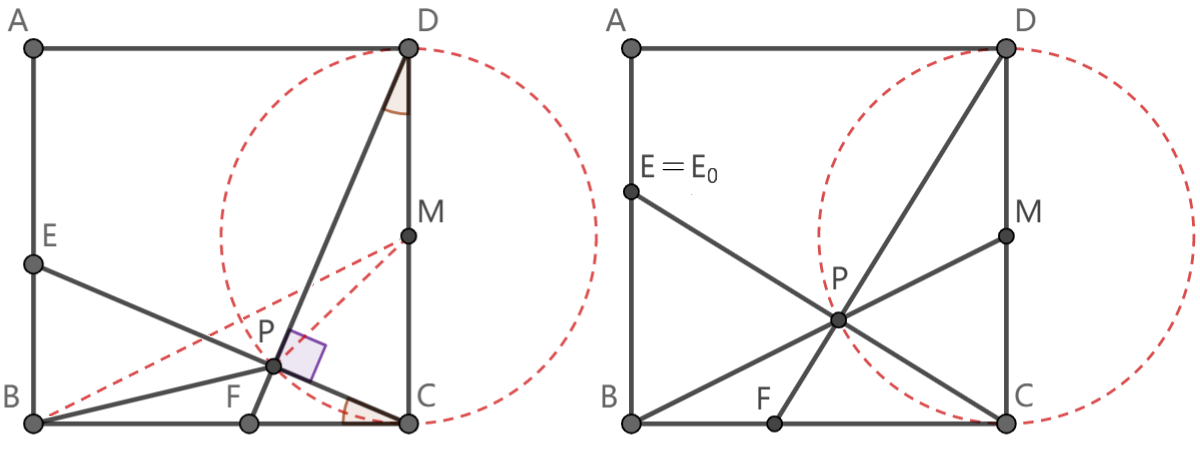
\includegraphics[width=0.8\textwidth]{不变量1.png}
\end{figure}

\begin{so}
    任何时刻,总有$\triangle EBC \simeq \triangle FCD$。因此$\angle PCB = \angle PDC$,$\angle CPD$为直角。这说明$P$总在以$CD$为直径的圆上,
    即$E$运动时,$P$到$CD$中点$M$的距离总为$4$。也就是说,$\triangle BPM$中,$|PM| = 4$、$|BM| = 4\sqrt{5}$都是定值。于是
    $$ |BP| \geqslant |BM| - |PM| = 4\sqrt{5} - 4.$$
    这个最小值是可以达到的。作以$CD$为直径的圆,和线段$BM$交于点$Q$。延长$CQ$与$AB$交于$E_0$,则$E$运动到$E_0$时,$P=Q$,这时$B,P,M$三点共线,
    因此$|BP| = |BM| - |PM|$,达到最小值。
\end{so}

\begin{et}
    如图,点$P_1$在抛物线$y = \frac{x^2}{4}$上从左到右运动。直线$OP_2$垂直于$OP_1$,并且和抛物线交于点$P_2$。
    过原点$O$作$P_1P_2$的垂线,垂足为$D$。当$P_1$运动时,求点$D$的轨迹。
\end{et}

\begin{figure}[H] %this figure will be at the right
    \vspace{4pt}
    \centering
    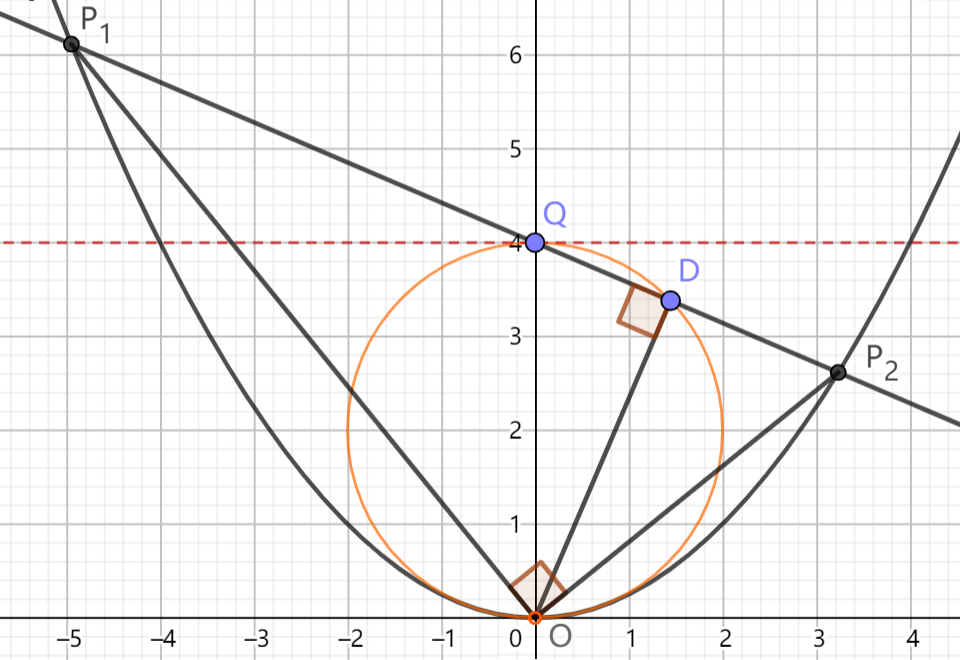
\includegraphics[width=0.6\textwidth]{不变量2.png}
\end{figure}

\begin{so}
    选几个不同的$P_1$点,作对应的直线$P_1P_2$。通过观察,可以发现这些点和$y$轴似乎交于同一点。猜测这是一个不变量。
    给定$P_1$,连接$P_1P_2$,交$y$轴于点$Q$。设直线$OP_1$的斜率为$a$,则它的方程为
    $$ y = ax. $$
    和抛物线方程联立求解,得到$P_1$坐标为$(a, \,\, \frac{a^2}{4})$。
    设直线$OP_2$斜率为$b$,则它的方程为
    $$ y = bx. $$
    同理解得$P_1$坐标为$(b, \,\, \frac{b^2}{4})$。于是$P_1P_2$的两点式方程为:
    $$ (x - a)(\frac{b^2}{4} - \frac{a^2}{4}) - (y - \frac{a^2}{4})(b - a) = 0$$
    令$x=0$,就得到直线$P_1P_2$和$y$轴交点的纵坐标:$y_Q = -\frac{ab}{4}$。
    由于$OP_1 \perp OP_2$,两者的方向向量内积为$0$。
    分别选方向向量$(1,\,\,\frac{a}{4})$、$(1,\,\,\frac{b}{4})$,就得到$1 + \frac{ab}{16} = 0$,即$ab = -16$。代入$Q$的纵坐标,
    就得到$y_Q = 4$。即$P_1P_2$与$y$轴的交点总是$Q(0,\,\,4)$。

    过$O$作$P_1P_2$的垂线,垂足为$D$,那么$\triangle ODQ$是直角三角形,$\angle ODQ$是直角。
    因此$D$总在以$OQ$为直径的圆:$x^2 + y(y-4) = 0$上。

    另一方面,给定以$OQ$为直径的圆上一点$D\neq Q$,连接$DQ$,交抛物线于两点:$P_1,P_2$。
    $DQ$的两点式方程为:
    $$ (x - x_D)(4 - y_D) - (y - y_D)(0 - x_D) = 0.$$
    将$y = \frac{x^2}{4}$代入,得到关于$x$的一元二次方程:
    $$ \frac{x_D}{4}x^2 + \left(4 - y_D\right)x - 4x_D = 0.$$
    只要$x_D\neq 0$,二次方程的判别式:
    $$ (4 - y_D)^2 - 4\cdot \frac{x_D}{4}\cdot(- 4x_D) = (4 - y_D)^2 + 4x_D^2 > 0.$$
    于是方程总有两个解。它的两个解就是$P_1,P_2$的横坐标$a,b$。因此根据根与系数的关系,$P_1,P_2$的横坐标乘积为
    $$ab = -4x_D \div \frac{x_D}{4} = -16.$$
    而$P_1,P_2$的纵坐标分别是$\frac{a^2}{4}$、$\frac{b^2}{4}$,于是两直线方向向量的内积为:
    $$ ab + \frac{a^2}{4}\cdot\frac{b^2}{4} = ab(1 + \frac{ab}{16}) = 0.$$
    即$OP_1 \perp OP_2$。
    
    如果$D=Q$,则$OD$垂直于抛物线上两点:$P_1(-4,\,\,4)$和$P_2(4,\,\,4)$的连线。
    可以验证$OP_1\perp OP_2$。于是点$Q$也在轨迹上。
    
    综上可知,一方面$D$的轨迹总在以$OQ$为直径的圆上。另一方面,除了原点$O$,以$OQ$为直径的圆都在$D$的轨迹上。
    因此,$D$的轨迹是:
    $$\{(x,\,\,y) \, | \, x^2 + y(y-4) = 0, \,\, (x,\,\,y)\neq (0,\,\,0)\}.$$
\end{so}

% TODO 补上习题
\section{平面形的变换}
% 平移。缩放和位似。反射和对称。旋转。变换的复合。
点运动形成轨迹。平面形,作为点的集合,其运动称为变换。我们熟悉的变换包括平移、缩放和旋转。
下面我们从点集运动的角度讨论平面形的各种变换。

设平面形为点集$S$,那么它的变换可以用二元映射$f$表示:
\begin{align}
    f: \,\, S\times[0,\,\,1] \,\,&\rightarrow \mathbb{R}^2 \notag \\
    (\mathbf{s},\,\, t) \quad &\mapsto f(\mathbf{s},\,\,t) \notag
\end{align}
具体来说,对$S$中每一点$\mathbf{s}$,$f$都定义了它的运动:$t\,\,\mapsto f(\mathbf{s},\,\,t)$。

比如,设$S$是以$(0,\,\,0)$、$(1,\,\,0)$、$(1,\,\,1)$、$(0,\,\,1)$为顶点的正方形(下面称为标准单位正方形)。
定义变换
$$f:\,\, (\mathbf{s}, \,\,t) \mapsto \mathbf{s} + t(0.5, \,\, -0.5). $$
$f$表示正方形中每一点$\mathbf{s}$沿着方向向量$(0.5, \,\, -0.5)$直线运动,即按该向量平移。
比如点$(0.2,\,\,0.35)$就沿着该方向直线运动到$(0.7, \,\,-0.15)$。

\begin{figure}[h] %this figure will be at the right
    \vspace{4pt}
    \centering
    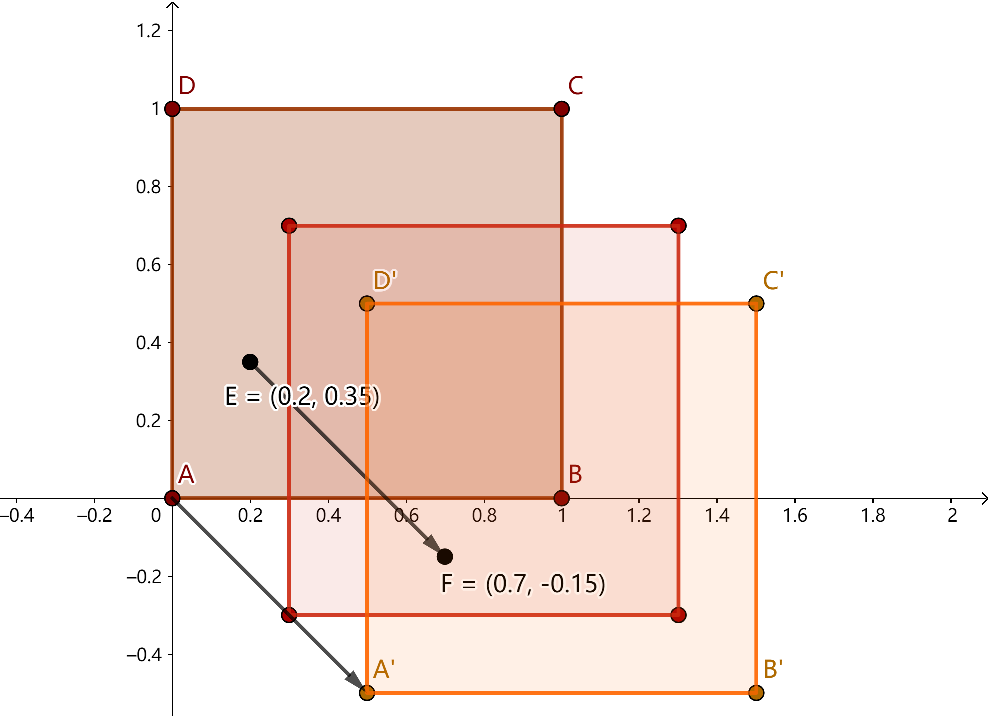
\includegraphics[width=0.6\textwidth]{平移变换例1.png}
\end{figure}

另一方面,对给定的$t$,我们可以定义$S(t) = \{f(\mathbf{s},\,\,t) \, | \, \mathbf{s}\in S\}$为变换的过程中,
$S$在$t$时刻的样子。上一个例子中,$S(0.6)$就是一个以$(0.3,\,\,-0.3)$、$(1.3,\,\,-0.3)$、
$(1.3,\,\,0.7)$、$(0.3,\,\,0.7)$为顶点的正方形。

从例子中可以看到,图形$S$按向量$U$的\textbf{平移变换}可以表示为:
\begin{align}
    \mathrm{Py}_U: \,\, S\times[0,\,\,1] \,\,&\rightarrow \mathbb{R}^2 \notag \\
    (\mathbf{s},\,\, t) \quad &\mapsto \mathbf{s} + tU. \notag
\end{align}

平移变换不改变图形的大小和形状,只改变图形的位置。大部分的变换对图形的大小、形状和位置都有改变。比如给定一个长度为$1$的向量(称为单位向量)$\mathbf{u}$,
考虑以下变换:
\begin{align}
    \mathrm{Ty}_\mathbf{u}: \,\, S\times[0,\,\,1] \,\,&\rightarrow \mathbb{R}^2 \notag \\
    (\mathbf{s},\,\, t) \quad &\mapsto t(\mathbf{s}\,|\,\mathbf{u})\mathbf{u} + (1 - t)\mathbf{s}. \notag
\end{align}
用一个例子来看这个变换的作用。给定向量$\mathbf{u} = (1,\,\,0)$,考虑点$\mathbf{s}$在变换中的运动情况。对给定的点$\mathbf{s}$来说,
它运动的轨迹是线段:
$$\{t(\mathbf{s}\,|\,\mathbf{u})\mathbf{u} + (1 - t)\mathbf{s} \, | \, t\in[0,1]\}.$$
$t=0$时,点从初始位置出发。
$t=1$时,点到达$(\mathbf{s}\,|\,\mathbf{u})\mathbf{u}$。我们注意到,变换把任何点变为和$\mathbf{u}$共线的向量。

具体来说,如果设点$\mathbf{s}$的坐标为$(x,\,\,y)$,那么运动的终点为$(x,\,\,0)$。
直观上看,如果把$x$轴看作地面,那么$(x,\,\,0)$可以看作$(x,\,\,y)$在竖直阳光下的影子。
所以,我们把这样的变换称为(正)\textbf{投影变换}。指定一个方向,投影变换把点垂直投影到这个方向上,
把点集变为它在这个方向上的“影子”。用数学的语言来说,投影变换捕捉出点在指定方向的分量。
我们一般把$\mathbf{u}$称为投影变换的(单位)方向向量。

举例来说,设$S$是标准单位正方形,$S$中任一点$(x,\,\,y)$在变换中的运动为$t\,\,\mapsto (x,\,\,\ (1 - t)y)$。
因此,$S$在$t$时刻的样子$S(t)$是一个长为$1$,宽为$1 - t$的长方形,最终变成从原点到$(1,\,\,0)$的线段。
这就是标准单位正方形在$(1,\,\,0)$方向的投影。

\begin{figure}[h] %this figure will be at the right
    \vspace{4pt}
    \centering
    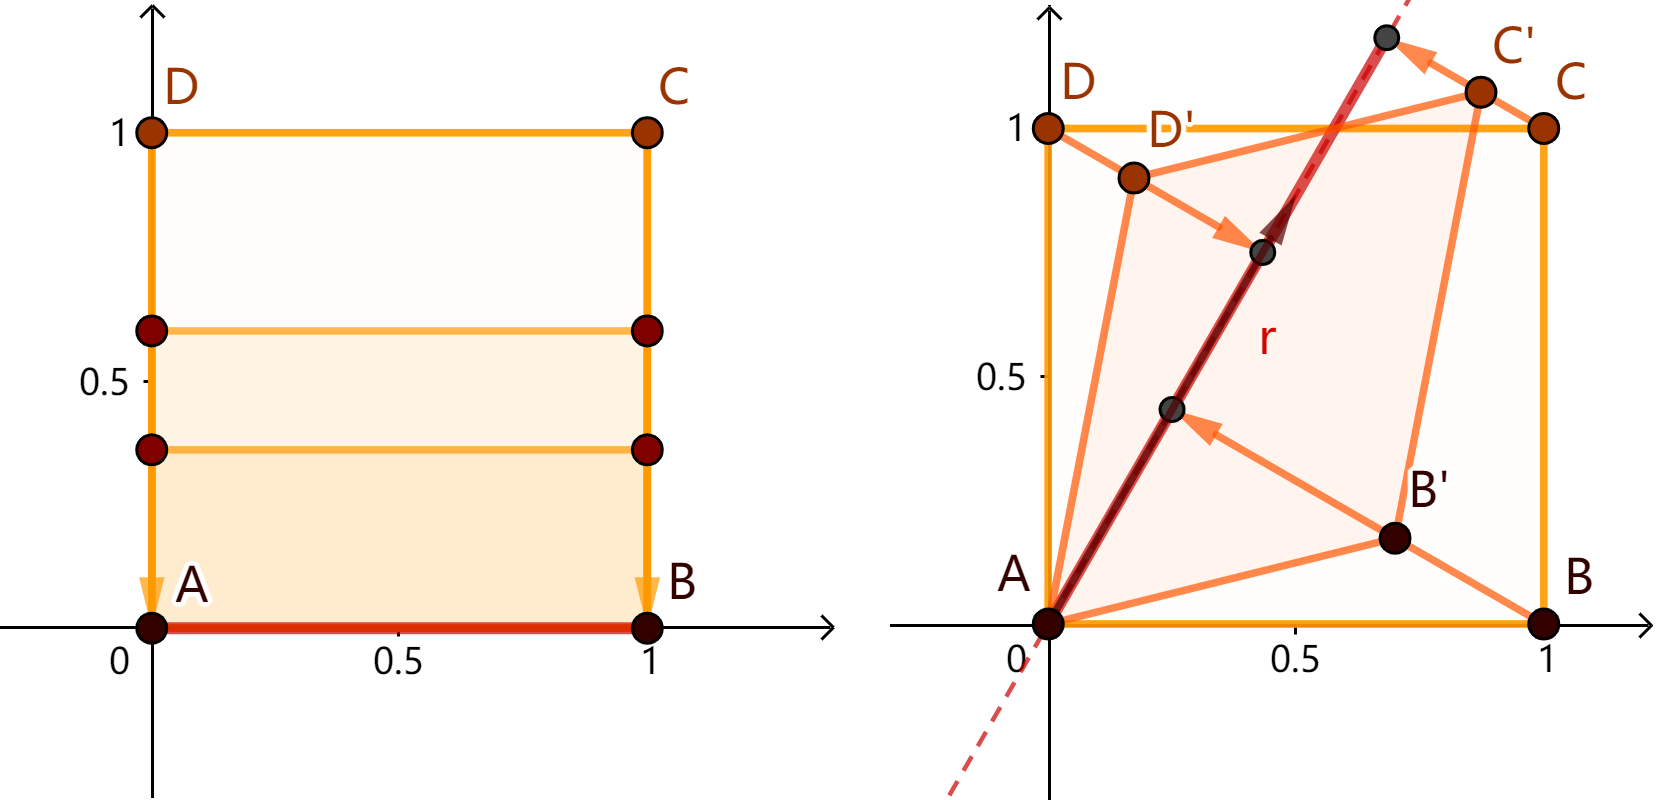
\includegraphics[width=0.75\textwidth]{投影变换例1.png}
\end{figure}

如果方向向量换成$(\frac{1}{2},\,\,\frac{\sqrt{3}}{2})$,
那么$S$中任一点$(x,\,\,y)$在变换中的运动为
$$t\,\,\mapsto (x,\,\,\ y) + t\left(\frac{\sqrt{3}}{4}y - \frac{3}{4}x,\,\,\ \frac{\sqrt{3}}{4}x - \frac{1}{4}y\right).$$
因此$t=1$时,$(x,\,\,y)$最终运动到点$\left(\frac{1}{2}x + \frac{\sqrt{3}}{2}y\right)(\frac{1}{2},\,\,\frac{\sqrt{3}}{2})$。
我们知道$x,\,\,y\in[0,1]$,因此$\frac{1}{2}x + \frac{\sqrt{3}}{2}y$最小为$0$,最大为$\frac{\sqrt{3}+1}{2}$。
也就是说,$S$变为从原点到$(\frac{\sqrt{3} + 1}{4},\,\,\frac{3 + \sqrt{3}}{4})$的线段。
这就是标准单位正方形在$(\frac{1}{2},\,\,\frac{\sqrt{3}}{2})$方向的投影。

另一种简单的变换是\textbf{位似变换}。
\textbf{位似}是一种特殊的相似关系。
举例来说,设$\triangle ABC$相似于$\triangle A'B'C$。
如果直线$AA'$、$BB'$、$CC'$交于一点$U$,就说两个三角形位似,$U$是\textbf{位似中心}。

位似变换可以表示为:
\begin{align}
    \mathrm{Ws}_{(U, \,\,k)}: \,\, S\times[0,\,\,1] \,\,&\rightarrow \mathbb{R}^2 \notag \\
    (\mathbf{s},\,\, t) \quad &\mapsto \mathbf{s} + t(1 - k)(U - \mathbf{s}). \notag
\end{align}
其中$U$是位似中心,$k$是终点时图形与初始图形的相似比。
我们说$S$以$U$为中心放缩,最终变成原来$k$倍大小。
从$S$中一点$\mathbf{s}$来看,它从$\mathbf{s}$出发,不断向$U$运动,最终到达$k\mathbf{s} + (1 - k)U$。

\begin{wrapfigure}[9]{r}{0.42\textwidth} %this figure will be at the right
    \vspace{-12pt}
    \flushright
    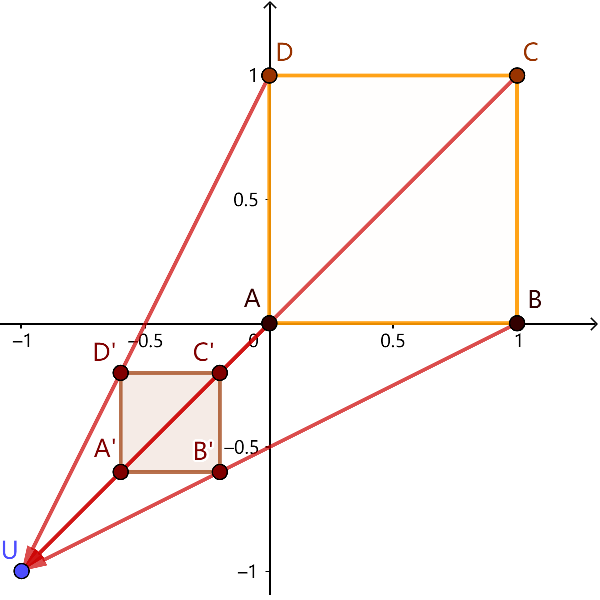
\includegraphics[width=0.4\textwidth]{位似变换例1.png}
\end{wrapfigure}

举例来说。设$S$是标准单位正方形,四个顶点分别是$A(0,\,\,0)$、$B(1,\,\,0)$、$C(1,\,\,1)$、$D(0,\,\,1)$。
指定位似中心$U(-1,\,\,-1)$,相似比$k=0.4$。于是位似变换中$A$沿直线运动到$A'(-0.6,\,\,-0.6)$,$B$沿直线运动到$B'(-0.2,\,\,-0.6)$。
线段$AB$上一点$(x,\,\,0)$沿直线运动到$(0.4x - 0.6, \,\, -0.6)$。于是线段$AB$变成线段$A'B'$。
同理线段$BC$、$CD$、$DA$变成线段$B'C'$、$C'D'$、$D'A'$,其中$C'=(-0.2,\,\, -0.2)$,$D'=(-0.6,\,\,-0.2)$。
于是标准单位正方形$S$变成边长为$0.4$的正方形$A'B'C'D'$。

我们学习过点和图形的轴对称。把图形变成它的轴对称图形,这样的变换叫做\textbf{反射变换}。
反射变换可以表示为:
\begin{align}
    \mathrm{Fs}_\mathbf{u}: \,\, S\times[0,\,\,1] \,\,&\rightarrow \mathbb{R}^2 \notag \\
    (\mathbf{s},\,\, t) \quad &\mapsto 2t(\mathbf{s}\,|\,\mathbf{u})\mathbf{u} + (1 - 2t)\mathbf{s}. \notag
\end{align}
其中$\mathbf{u}$是对称轴所在直线的单位方向向量。

\begin{wrapfigure}[7]{r}{0.42\textwidth} %this figure will be at the right
    \vspace{-42pt}
    \flushright
    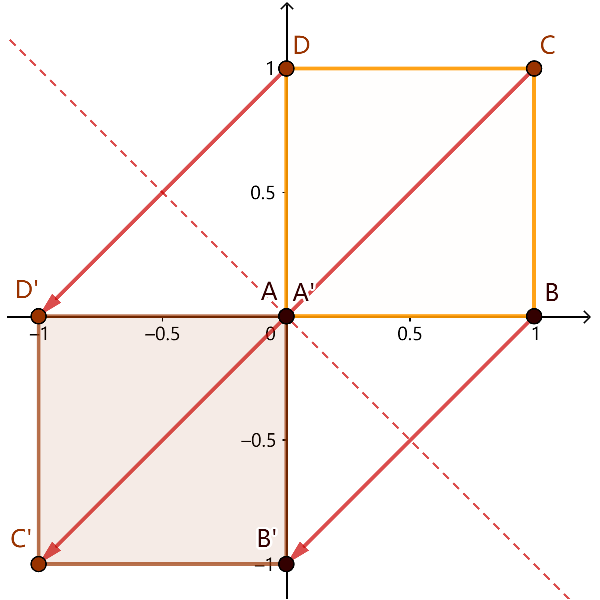
\includegraphics[width=0.4\textwidth]{反射变换例1.png}
\end{wrapfigure}

举例来说,设方向向量$\mathbf{u} = \left(-\frac{\sqrt{2}}{2},\,\,\frac{\sqrt{2}}{2}\right)$,标准单位正方形经历变换$\mathrm{Fs}_\mathbf{u}$,其中的点$(x,\,\,y)$的运动为:
\begin{align}
    t \,\, \mapsto &\quad (t(x-y), \,\,t(y-x)) + (1 - 2t)(x, \,\,y) \notag \\
    & = (x, \,\,y) - t(x+y)(1, \,\, 1) \notag
\end{align}
$t=1$时,点$(x,\,\,y)$到达$(-y,\,\,-x)$,即它关于直线$x+y=0$的对称点。于是$\mathrm{Fs}_\mathbf{u}$将标准单位正方形变换为它关于$x+y=0$的对称图形,即
以$(0,\,\,0)$、$(0,\,\,-1)$、$(-1,\,\,-1)$、$(-1,\,\,0)$为顶点的正方形。

最后来看\textbf{旋转变换}。旋转变换指的是以给定角的顶点为中心,把某个图形按该角旋转。

首先来看一点的旋转。
给定角$\alpha$,顶点为$U$。平面中一点$P$关于$\alpha$旋转的结果,
是唯一使得$\angle PUQ = \alpha$且$|UP| = |UQ|$的点$Q$\footnote{如果$P=U$,则旋转后仍为$P$。}。
以$U$为圆心,以$|UP|$为半径作圆,则$P$沿圆弧运动到$Q$。
顶点$U$称为\textbf{旋转中心},$\alpha$称为\textbf{旋转角}。

最简单的情况是$U$为原点。这时,设点$P$的坐标为$(x,\,\,y)$,$|UP| = r = \sqrt{x^2 + y^2}$。
取$x$轴上的点$S(1,\,\,0)$为基准,设$\angle SUP = \theta$,容易验证,$|x| = r|\cos{\theta}|$,
$|y| = r|\sin{\theta}|$。对比各个象限中$x$、$y$和$\cos{\theta}$、$\sin{\theta}$的正负号,可以发现:
任何情况下,$x$总与$\cos{\theta}$同正负,$y$总与$\sin{\theta}$同正负。

\begin{tm}
    设$P(x,\,\,y)$是平面上原点外一点,设以$x$轴正半轴为始边、射线$OP$为终边的角为$\theta$,则
    $$ x = r\cos{\theta},\quad y = r\sin{\theta}.$$
    其中$r = \sqrt{x^2 + y^2}$。
\end{tm}
这个定理将点的坐标和角度联系起来,是我们讨论平面角度和旋转问题的关键。 

\begin{wrapfigure}[7]{r}{0.36\textwidth} %this figure will be at the right
    \vspace{-40pt}
    \flushright
    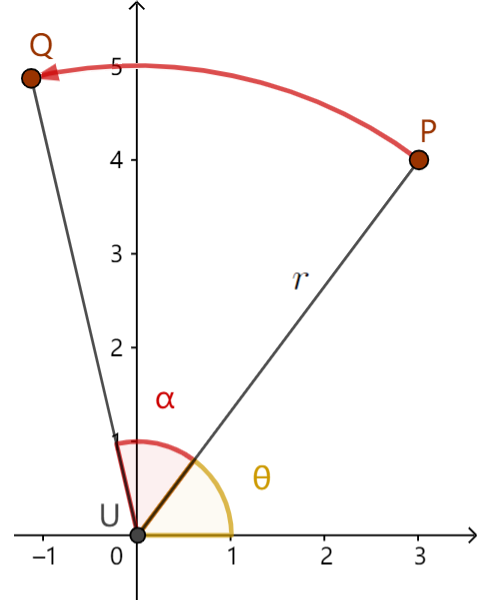
\includegraphics[width=0.3\textwidth]{旋转变换例1.png}
\end{wrapfigure}

如果将$P$按角$\alpha$旋转,那么与$x$轴正半轴张成的角应该从$\theta$变为$\theta + \alpha$。
用角度来描述旋转运动,就是:$t \mapsto \theta + t\alpha$。回到点的具体位置,
$t$时刻$UP$的长度仍然是$r$,而角度是$\theta + t\alpha$,因此,它的坐标是$(r\cos{(\theta + t\alpha)},\,\,r\sin{(\theta + t\alpha)})$。
使用和角公式,可以将它转化为:
$$(r\cos{\theta}\cos{(t\alpha)} - r\sin{\theta}\sin{(t\alpha)},\,\,r\cos{\theta}\sin{(t\alpha)} + r\sin{\theta}\cos{(t\alpha)}).$$
用$x,y$表示,旋转运动就是:
$$ t \mapsto \left(x\cos{(t\alpha)} - y\sin{(t\alpha)}, \,\,x\sin{(t\alpha)} + y\cos{(t\alpha)}\right).$$

如果$U$不是原点,坐标是$(x_U, \,\,y_U)$,那么$\vv{UP} = (x - x_U, \,\, y - y_U)$。$\vv{UP}$旋转变为$\vv{UQ}$的运动和前面类似。
因此通过$Q = U + \vv{UQ}$就可得到$Q$。于是旋转运动可以表示为:
\begin{align}
    t \mapsto (x_U,\,\,y_U) + &\big((x - x_U)\cos{(t\alpha)} - (y - y_U)\sin{(t\alpha)},\notag \\
    &\,\,\,(x - x_U)\sin{(t\alpha)} + (y - y_U)\cos{(t\alpha)}\big).\notag
\end{align}

因此,旋转变换可以表示为:
\begin{align}
    \mathrm{Xz}_{(U,\,\,\alpha)}: \,\, S\times[0,\,\,1] \,\,&\rightarrow \mathbb{R}^2 \notag \\
    ((x,\,\,y),\,\, t) \quad &\mapsto (x_U,\,\,y_U)+\big((x - x_U)\cos{(t\alpha)} - (y - y_U)\sin{(t\alpha)},\notag \\
    &\qquad\qquad\qquad\quad(x - x_U)\sin{(t\alpha)} + (y - y_U)\cos{(t\alpha)}\big). \notag
\end{align}

\begin{wrapfigure}[7]{r}{0.42\textwidth} %this figure will be at the right
    \vspace{-22pt}
    \flushright
    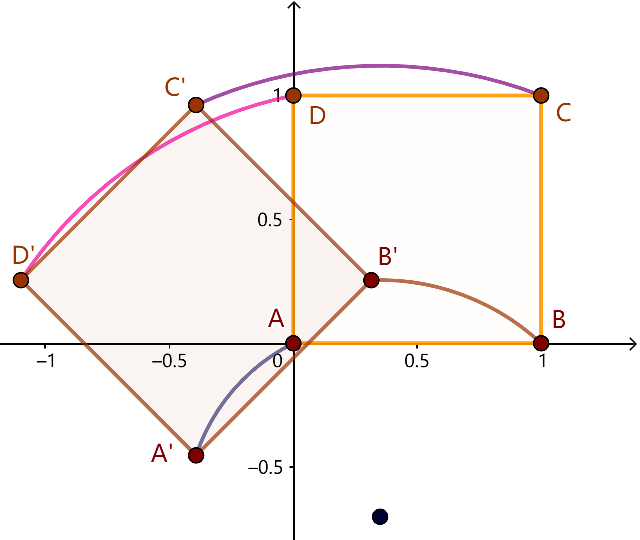
\includegraphics[width=0.4\textwidth]{旋转变换例2.png}
\end{wrapfigure}

可以看到,旋转变换的表示形式繁琐。这是向量和直角坐标系的性质决定的。

直角坐标系与向量的共线性质和内积相关。共线性、内积的基本性质都只和向量的加法、数乘运算相关。
而向量定义中的加法和数乘运算,分别对应平移和放缩变换。
向量定义中并没有与旋转对应的运算,共线性、内积的性质也不包括旋转,
因此,要通过向量在直角坐标系下的坐标表示旋转,自然不是简单的事情。

一种折中的方法是使用极坐标系。极坐标系是科学家研究南北极地时发明的。在南北极圈中,各条经线汇于极点。
人们发现,使用到极点的距离和经度描述位置,比使用经纬度更精确、更方便。

\begin{figure}[h] %this figure will be at the right
    % \vspace{4pt}
    \centering
    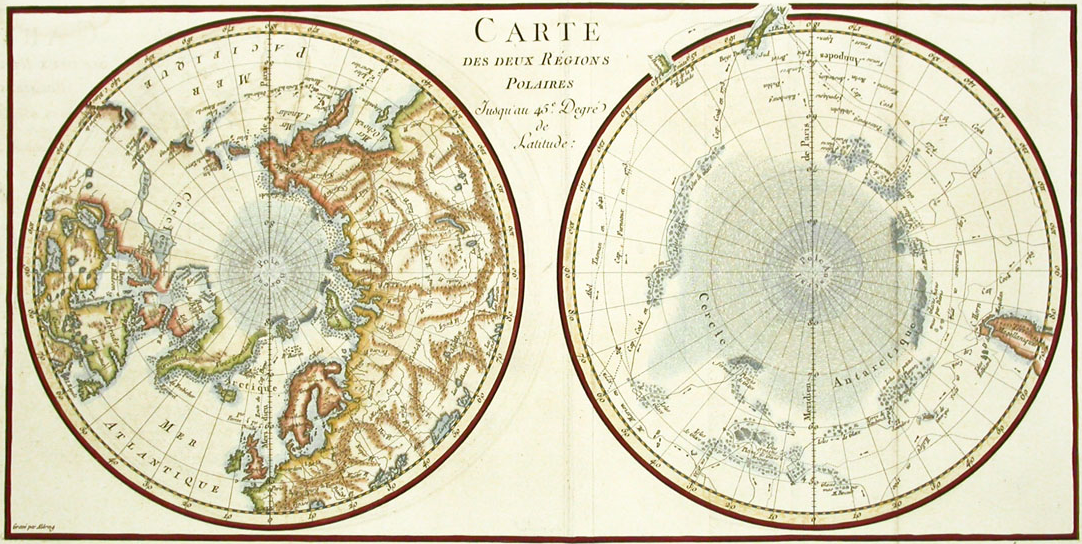
\includegraphics[width=0.8\textwidth]{极坐标例1南北极地图2.jpg}
    \caption*{\texttt{使用极坐标系的极地地图}}
\end{figure}
如下图所示,一点$A$在极坐标系中的坐标称为极坐标,它由模长和辐角组成。模长就是点$A$到原点$O$的距离,
辐角是$x$轴正半轴到$\vv{OA}$所构成的角。比如,直角坐标系中坐标为$(1,\,\,1)$的点,在极坐标系中可以表示为
$(\sqrt{2},\,\, 45^\circ)$。

\begin{figure}[h] %this figure will be at the right
    \vspace{4pt}
    \centering
    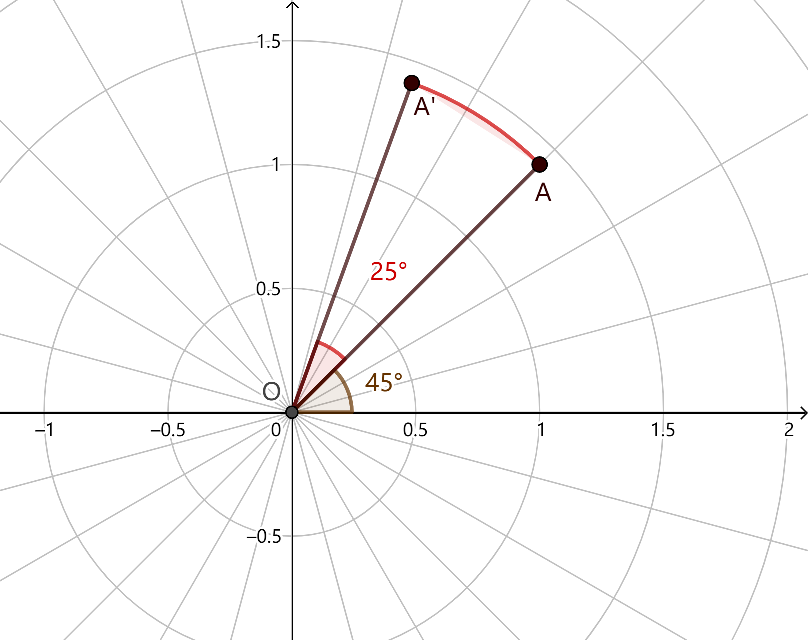
\includegraphics[width=0.5\textwidth]{极坐标例2.png}
\end{figure}

使用极坐标系,可以比较方便地描述以原点为中心的旋转运动。比如,直角坐标系中,
点$(1,\,\,1)$以原点为中心顺时针旋转$25^\circ$,可以用极坐标系描述为:
$$ t\,\, \mapsto (\sqrt{2}, \,\, 45^\circ + t \cdot 25^\circ)$$
然而,用极坐标系描述平移、放缩等运动就比较复杂。因此,用极坐标描述以非原点为中心的旋转,仍然繁琐。

\begin{et}
    直角坐标系中,设$A$、$B$坐标分别为$(2,\,\, -1)$、$(1,\,\, 3)$。考虑线段$AB$,
    以原点为中心,将其旋转$45^\circ$,然后以原点为中心,将其放大为原来的$2$倍,再按$(0,\,\, -2)$平移。最终得到的图形是什么?
\end{et}
\begin{so}
    线段$AB$经历了$3$个变换,分别可以记为$\mathrm{Xz}_{(O,\,\,\alpha)}$、$\mathrm{Ws}_{(O,\,\, 2)}$和$\mathrm{Py}_{M}$,
    其中$\alpha = 45^\circ$,$M = (0,\,\,-2)$。

    首先看第一个变换。$\mathrm{Xz}_{(O,\,\,\alpha)}$可以表示为:
    \begin{align}
        ((x,\,\,y),\,\, t) \,\,\, \mapsto \left(x\cos{(t\alpha)} - y\sin{(t\alpha)},\,\,x\sin{(t\alpha)} + y\cos{(t\alpha)}\right). \notag
    \end{align}
    因此$t=1$时,$(x,\,\,y)$运动到$\left(\frac{\sqrt{2}}{2}(x-y),\,\,\frac{\sqrt{2}}{2}(x+y)\right).$
    计算可得,$A$经过旋转变成$A_1 = \left(\frac{3\sqrt{2}}{2},\,\, \frac{\sqrt{2}}{2}\right)$,
    $B$经过旋转变成$B_1 = \left(-\sqrt{2},\,\, 2\sqrt{2}\right)$。线段$AB$经过旋转变为线段$A_1B_1$。

    接着进行第二个变换。$\mathrm{Ws}_{(O,\,\, 2)}$可以表示为:
    \begin{align}
        (\mathbf{s},\,\, t) \,\,\, \mapsto \mathbf{s} - t(O - \mathbf{s}). \notag
    \end{align}
    因此$t=1$时,$\mathbf{s}$运动到$2\mathbf{s}$。计算可得,$A_1$经过放缩变成$A_2 = \left(3\sqrt{2},\,\, \sqrt{2}\right)$,
    $B$经过放缩变成$B_2 = \left(-2\sqrt{2},\,\, 4\sqrt{2}\right)$。线段$A_1B_1$经过旋转变为线段$A_2B_2$。

    最后进行平移变换。$\mathrm{Py}_{M}$可以表示为:
    $$ (\mathbf{s},\,\, t) \,\,\, \mapsto \mathbf{s} + tM. $$
    因此$t=1$时,$\mathbf{s}$运动到$\mathbf{s} + M$。计算可得,点$A_2$经过平移变成$A_3 = \left(3\sqrt{2},\,\, \sqrt{2}-2\right)$,
    $B$经过平移变成$B_3 = \left(-2\sqrt{2},\,\, 4\sqrt{2}-2\right)$。线段$A_2B_2$经过旋转变为线段$A_3B_3$。

    综上所述,线段$AB$经过三个变换,最终得到线段$A_3B_3$。
\end{so}

\begin{sk}
    \mbox{}\\
    \indent 1. 如何描述图形关于某点的中心对称变换? \\
    \indent 2. 如果一个变换的任意时刻,图形中任两点的距离不变,就说它是保距变换。本节提到的变换中,哪些变换是保距变换?\\
    \indent 3. 如果一个变换的任意时刻,图形中的角的角度不变,就说它是保角变换。本节提到的变换中,哪些变换是保角变换?
\end{sk}

\begin{xt}
    \mbox{}\\
    \indent 1. 将标准单位正方形以原点为中心,按$45^\circ$顺时针旋转,最终得到的图形是什么?详细描述这个变换。\\
    \indent 2. 设点$A$、$B$、$C$的坐标分别是$(0,\,\, 4)$、$(-1,\,\, 0)$、$(1,\,\,1)$。\\
    \indent 2.1. 以原点为中心,把$\triangle ABC$按$90^\circ$顺时针旋转,然后以原点为中心,将其放大为原来的$3$倍,再按$(-5, \,\, 0)$平移。最终得到的图形是什么?\\
    \indent 2.2. 把$\triangle ABC$按$\mathbb{R}\left(\frac{1}{2},\,\, \frac{\sqrt{3}}{2}\right)$作反射变换,再按$(0,\,\, 6)$平移。最终得到的图形是什么?\\
    \indent 2.3. 以原点为中心,把$\triangle ABC$分别按$30^\circ$、$120^\circ$顺时针旋转,然后投影到$\left(\frac{2\sqrt{5}}{5},\,\, -\frac{\sqrt{5}}{5}\right)$方向上。最终分别得到什么图形?\\
    \indent 3. 某工厂的机械臂要完成一个平面动作,可以简单描述为把端点为$A(1,\,\, 2)$、$B(-2,\,\, 1)$的线段,
    变换为端点为$A'(-4,\,\, 4)$、$B'(-4,\,\, -6)$的线段。机械臂可以进行$3$种操作:以原点为中心的旋转变换、按任一向量的平移变换、
    以线段一端为中心的位似变换。\\
    \indent 3.1. 请设计一种操作组合,把$AB$移动到$A'B'$。\\
    \indent 3.2. 请设计一种操作组合,把$AB$移动到$A'B'$,并确保$AB$的中点经过点$(-2,\,\, -2)$。\\
    \indent 3.3. 已知机械臂的每种操作成本。旋转变换的成本与线段中点经过的距离成正比,每单位长度$0.65$元;
    平移变换的成本和平移距离成正比,每单位长度$0.4$元;位似变换的成本和变换前后线段长度的差值成正比,每单位长度$0.8$元。请设计一种操作方式,使成本最低。\\
    \indent 3.4. 同上,如果要确保$AB$的中点经过点$(-2,\,\, -2)$,那么怎样操作成本最低?
\end{xt}

\chapter{从平面到立体}

我们已经初步了解了简单平面图形的性质。下面我们来认识立体形状。

我们生活的世界是立体空间。人类自身和自然万物,都是立体的。立体形状是我们最常接触的形状。
不过,人类的眼睛和大脑并不能直接处理立体形状,只能感知立体事物的平面图像,在大脑中还原事物的形状。
因此,人类总是通过平面图像来了解立体事物,通过平面图像还原、表现现实。

\begin{figure}[h] %this figure will be at the right
    \vspace{4pt}
    \centering
    
\includegraphics[width=1\textwidth]{景色1.jpg}
    \caption*{\texttt{平面图像与现实}}
\end{figure}

\section{多面体}
观察以下的物品,它们有什么相似之处?

\begin{figure}[h] %this figure will be at the right
    \vspace{4pt}
    \centering
    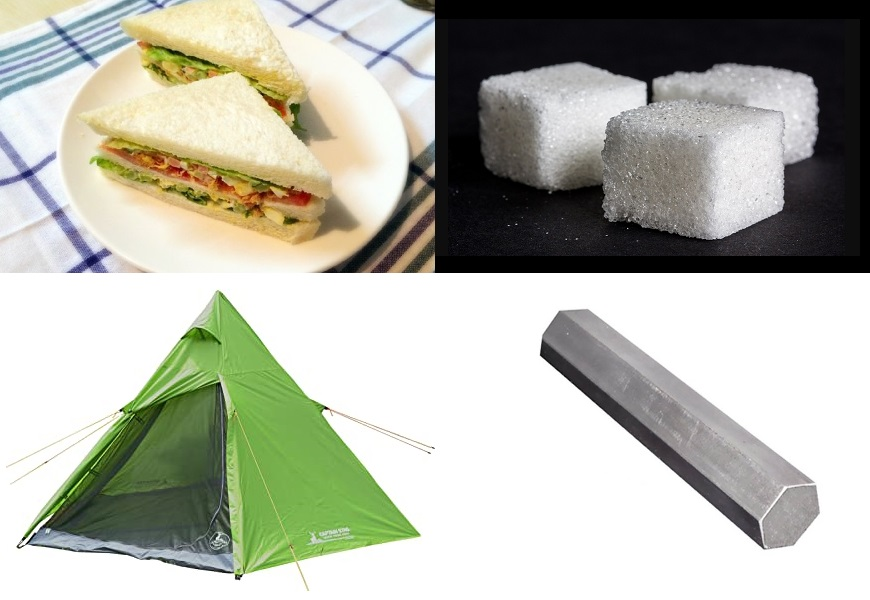
\includegraphics[width=0.6\textwidth]{多面体例1.jpg}
\end{figure}

如果立体形状是几个平面围成的,就说它是\textbf{多面体}。多面体的每个面都是多边形。

我们按照多面体的面数来称呼它。比如,由四个面围成的多面体叫四面体,由九个面围成的多面体叫九面体。

\begin{figure}[h] %this figure will be at the right
    \vspace{4pt}
    \centering
    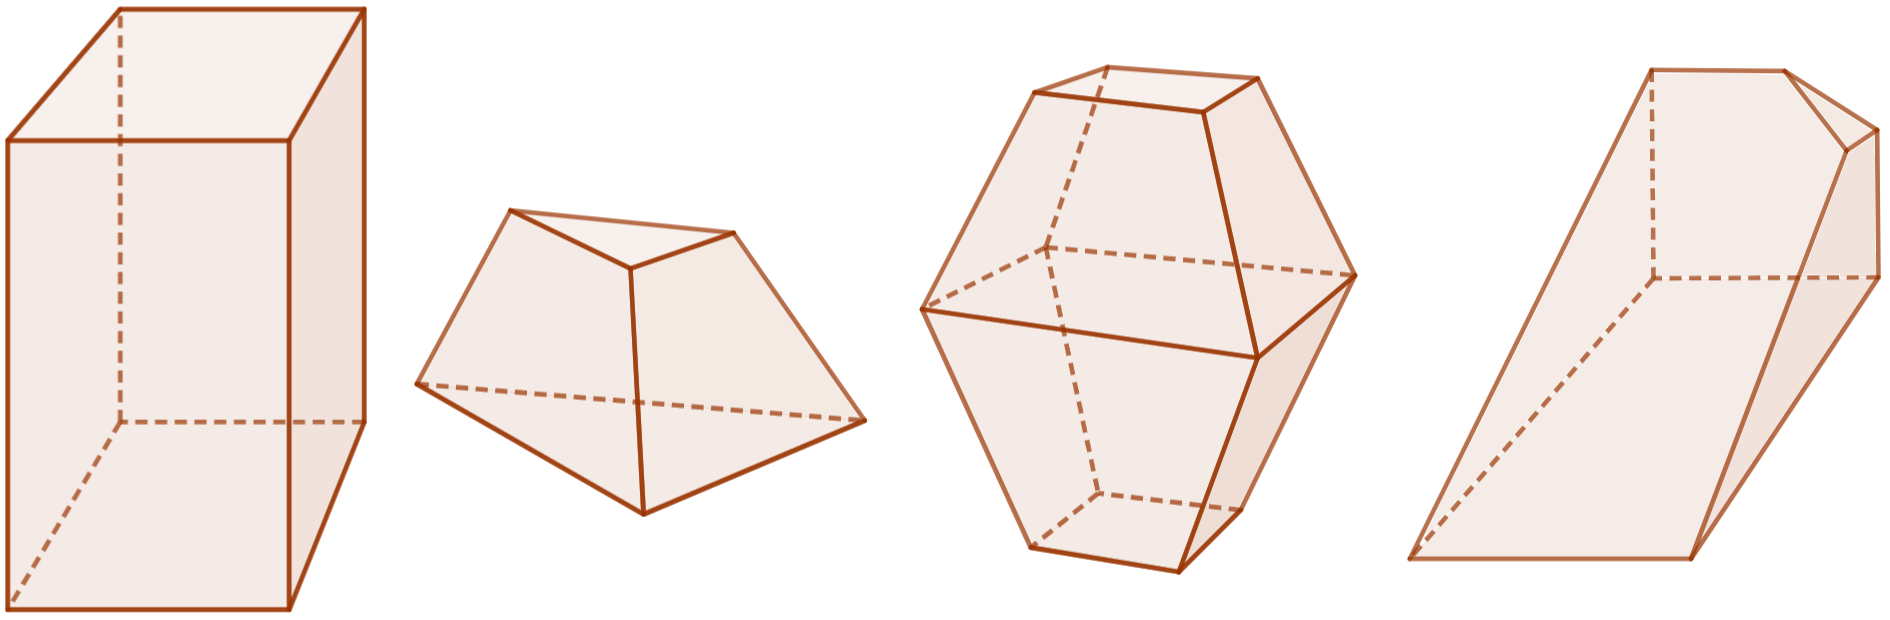
\includegraphics[width=0.8\textwidth]{多面体2.png}
\end{figure}

多面体相邻两面相交的部分总是线段,这些线段叫做\textbf{多面体的棱}。三条或以上的棱,交会在共同的端点上,
这些点也是多面体相邻的几个面的共同点,称为\textbf{多面体的顶点}。

数一数,上图中的多面体各有几个面?有几条棱?有几个顶点?

\begin{sk}
    \mbox{}\\
    \indent 1. 日常生活中,你还见过哪些多面体?\\
    \indent 2. 多面体的顶点有没有可能只是两条棱的共同端点?\\
    \indent 3. 多面体相邻两面的交点是否一定是线段?多面体的棱有没有可能是三个或以上的相邻面的共同部分?    
\end{sk}

\begin{wrapfigure}[3]{r}{0.29\textwidth} %this figure will be at the left
    \vspace{-50pt}
    \flushright
    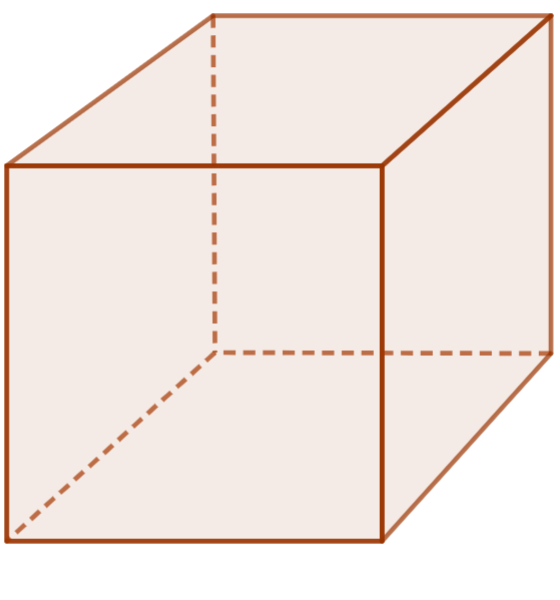
\includegraphics[width=0.25\textwidth]{正方体1.png}
\end{wrapfigure}

下面来认识几种特殊的多面体。

右图中的多面体由六个正方形组成。它叫做\textbf{正方体}或\textbf{正六面体}。
观察正方体,你能总结出什么特征?

\begin{wrapfigure}[4]{l}{0.3\textwidth} %this figure will be at the left
    \vspace{-20pt}
    \flushright
    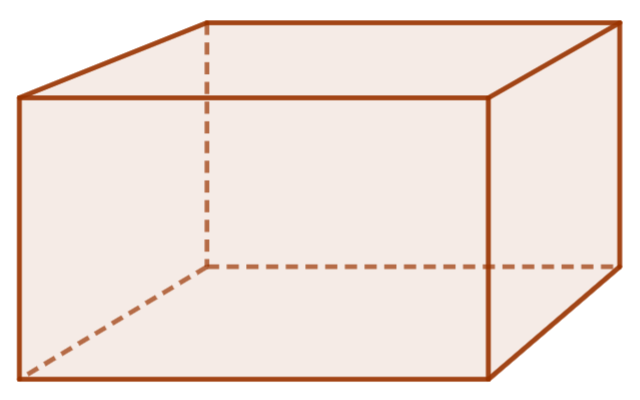
\includegraphics[width=0.25\textwidth]{长方体1.png}
\end{wrapfigure}

把正方体按某条棱的方向延长或压缩,得到的多面体叫做\textbf{长方体}。正方体就是一种特殊的长方体。
显然,长方体也是六面体。观察长方体,你能总结出什么特征?

\begin{sk}
    \mbox{}\\
    \indent 1. 正方体有几条棱?棱与棱之间有什么关系?\\
    \indent 2. 正方体有几个顶点?顶点与顶点之间有什么关系?\\
    \indent 3. 正方体是否是对称形状?你能说出正方体的哪些对称性质?长方体呢?
\end{sk}

观察下图中的多面体,它们有什么共同特征?

\begin{figure}[h] %this figure will be at the right
    \vspace{4pt}
    \centering
    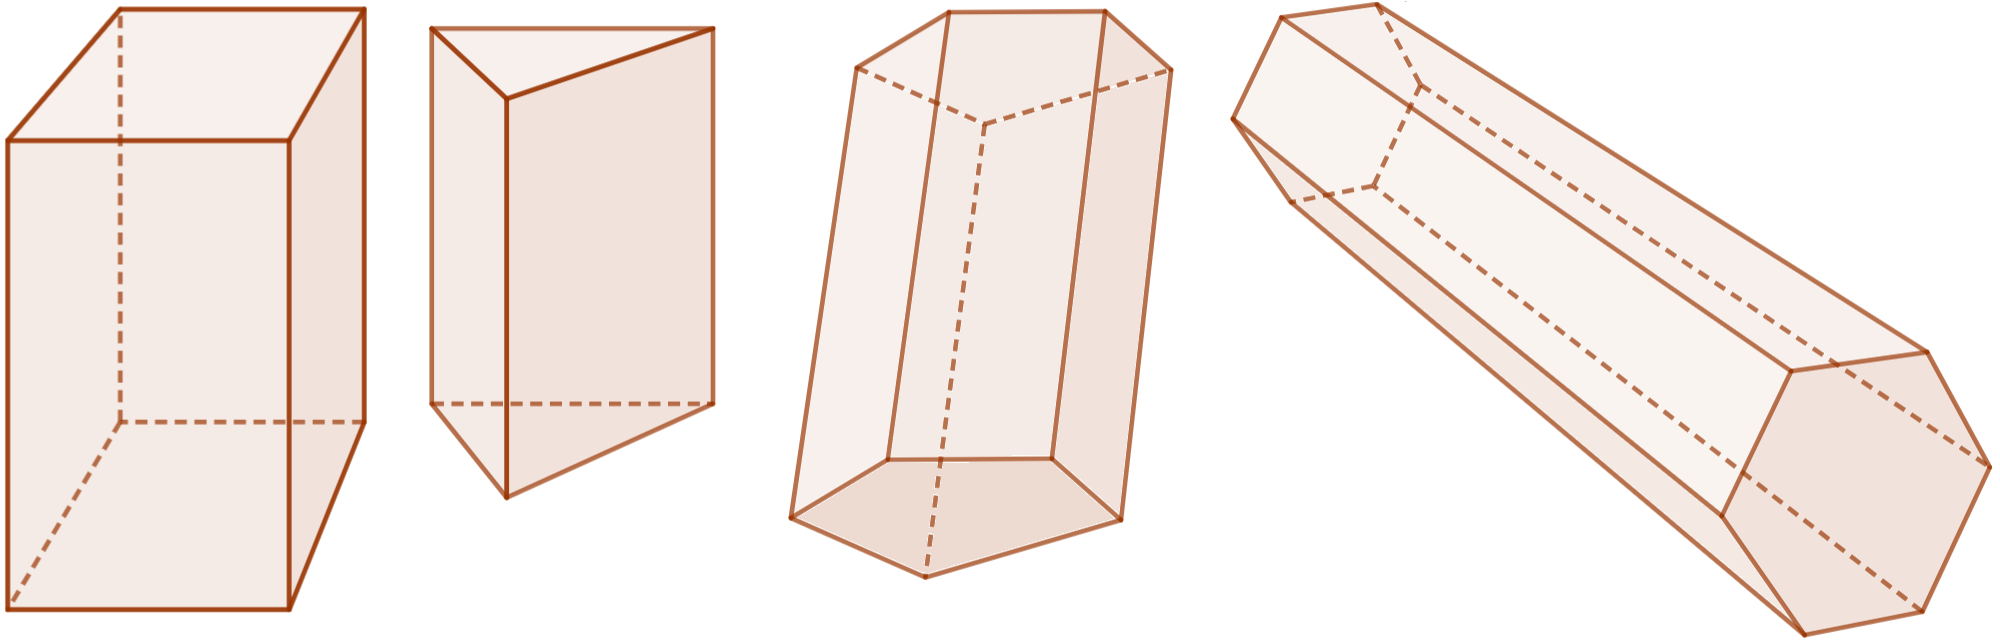
\includegraphics[width=0.8\textwidth]{棱柱1.png}
\end{figure}

把一个多边形朝指定方向平移,可以得到多面体。这样的多面体叫做\textbf{棱柱}。
平移的多边形叫做\textbf{棱柱的底面}。其它面叫做\textbf{棱柱的侧面}。

\begin{sk}
    \mbox{}\\
    \indent 1. 棱柱的侧面有什么特征?\\
    \indent 2. 正方体和长方体是棱柱吗?\\
    \indent 3. 你能说出生活中见过的棱柱吗?\\
    \indent 4.《九章算术》刘徽注:“邪(斜)解立方得两堑堵,邪解堑堵,其一为阳马,一为鳖臑,阳马居二,鳖臑居一,不易之率也。合两鳖臑成一阳马,合三阳马而成一立方,故三而一。”
    其中的“立方“就是正方体。已知“堑堵”和“阳马”是五面体、“鳖臑”是四面体,自行探究:刘徽说的“堑堵”、“阳马”、“鳖臑”分别是什么?如何理解刘徽说的话?
\end{sk}

\section{旋转体和球}

观察以下的物品,它们有什么相似之处?

\begin{figure}[h] %this figure will be at the right
    \vspace{4pt}
    \centering
    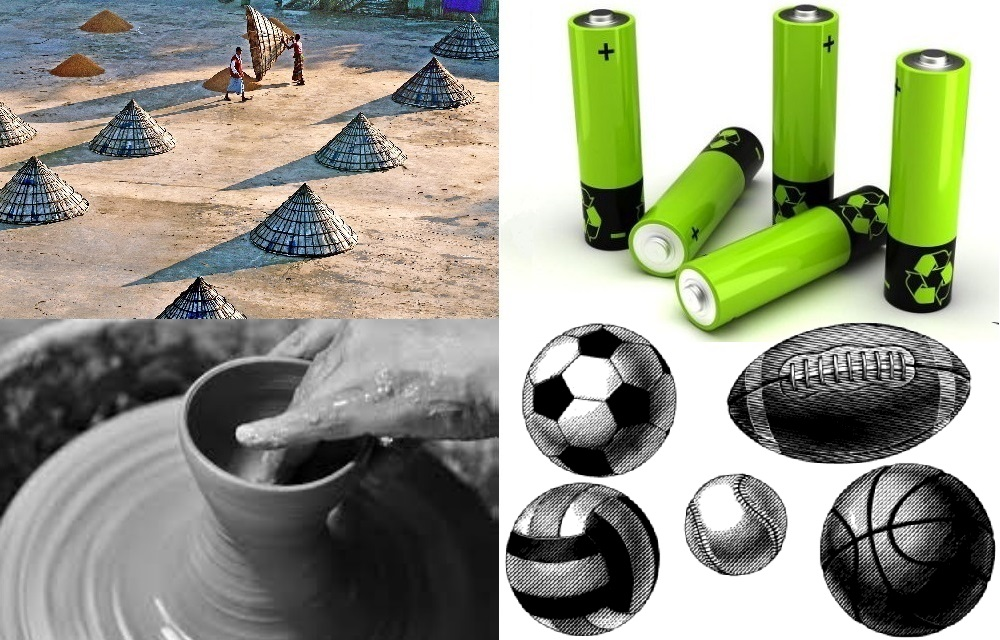
\includegraphics[width=0.8\textwidth]{旋转体例1.jpg}
\end{figure}

如果立体形状是某个平面图形绕着定轴旋转一周而成的,就说它是\textbf{旋转体}。

多面体可以是旋转体吗?

任何点绕定轴旋转一周,必然形成一个圆。考虑多面体表面的点,它们旋转之后是否能留在所属的平面上?

\begin{wrapfigure}[9]{r}{0.22\textwidth} %this figure will be at the left
    \vspace{-10pt}
    \flushright
    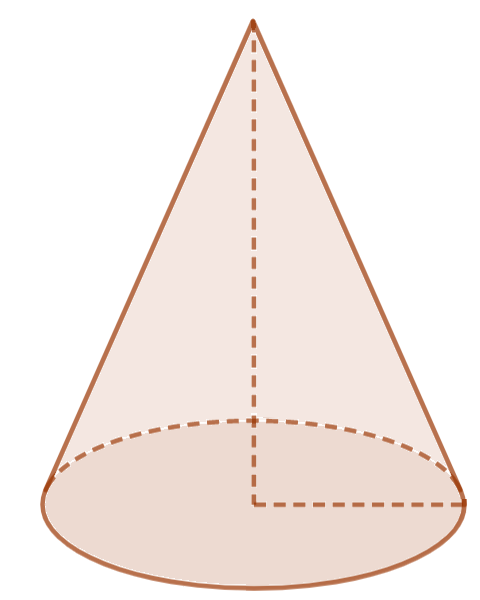
\includegraphics[width=0.2\textwidth]{圆锥1.png}

    \vspace{20pt}
    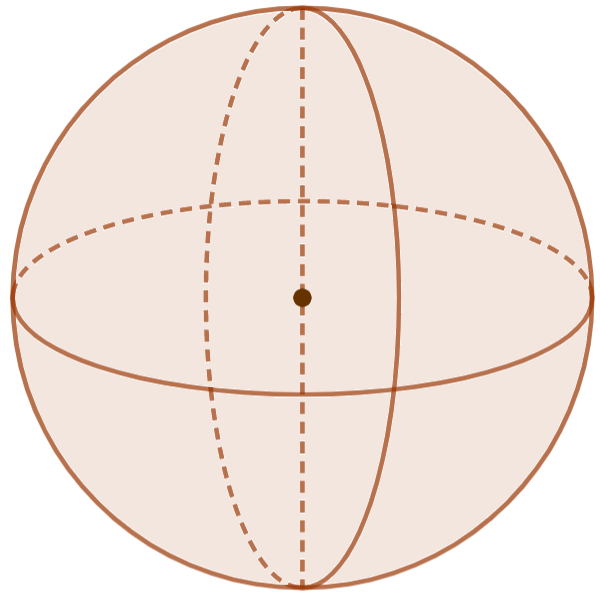
\includegraphics[width=0.2\textwidth]{球体1.png}
\end{wrapfigure}

观察右图中的旋转体,它有几个面?它的面和多面体的面有什么不同?

直角三角形绕着直角边所在的直线旋转一周,形成的立体形状叫做\textbf{圆锥}。圆锥有两个面,
一个面是平的,一个面是曲面。我们把平的面叫做\textbf{圆锥的底面},把曲面叫做\textbf{圆锥的侧面}。侧面的顶端叫做\textbf{圆锥的锥顶}。

矩形绕着它某条边所在的直线旋转一周,形成的立体形状叫做\textbf{圆柱}。圆柱有三个面,
其中两个面是平的,一个面是曲面。我们把平的面叫做\textbf{圆柱的底面},把曲面叫做\textbf{圆柱的侧面}。

\begin{wrapfigure}[6]{l}{0.22\textwidth} %this figure will be at the left
    \vspace{-16pt}
    \flushleft
    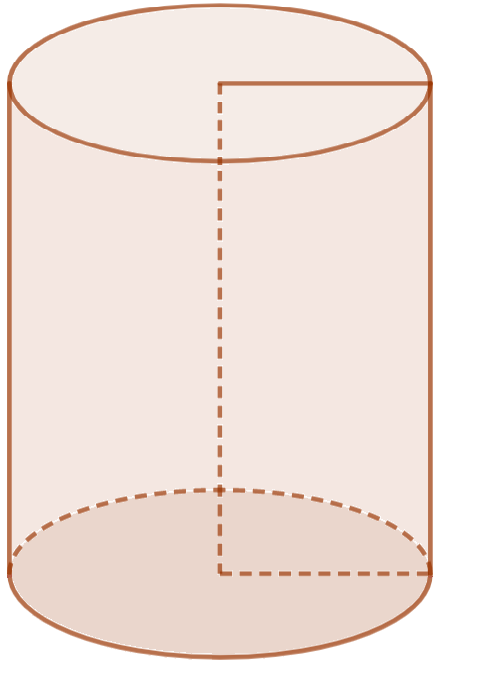
\includegraphics[width=0.2\textwidth]{圆柱2.png}
\end{wrapfigure}

圆形绕着过圆心的直线旋转一周,形成的立体形状叫做\textbf{球}或\textbf{球体}。球只有一个面,叫做\textbf{球面}。

\begin{sk}
    \mbox{}\\
    \indent 1. 日常生活中,你还见过哪些旋转体?\\
    \indent 2. 圆锥、圆柱的底面是什么形状?为什么?\\
    \indent 3. 圆柱和棱柱有什么相似之处?能不能用别的方式定义圆柱?\\
    \indent 4. 圆锥、圆柱和球是否是对称形状?你能说出它们的哪些对称性质?
\end{sk}

\section{在平面上表示立体形状}

让我们在平面上还原我们看到的立体事物。为什么下图中的$A$显得远,$B$显得近?

\begin{figure}[h] %this figure will be at the right
    % \vspace{4pt}
    \centering
    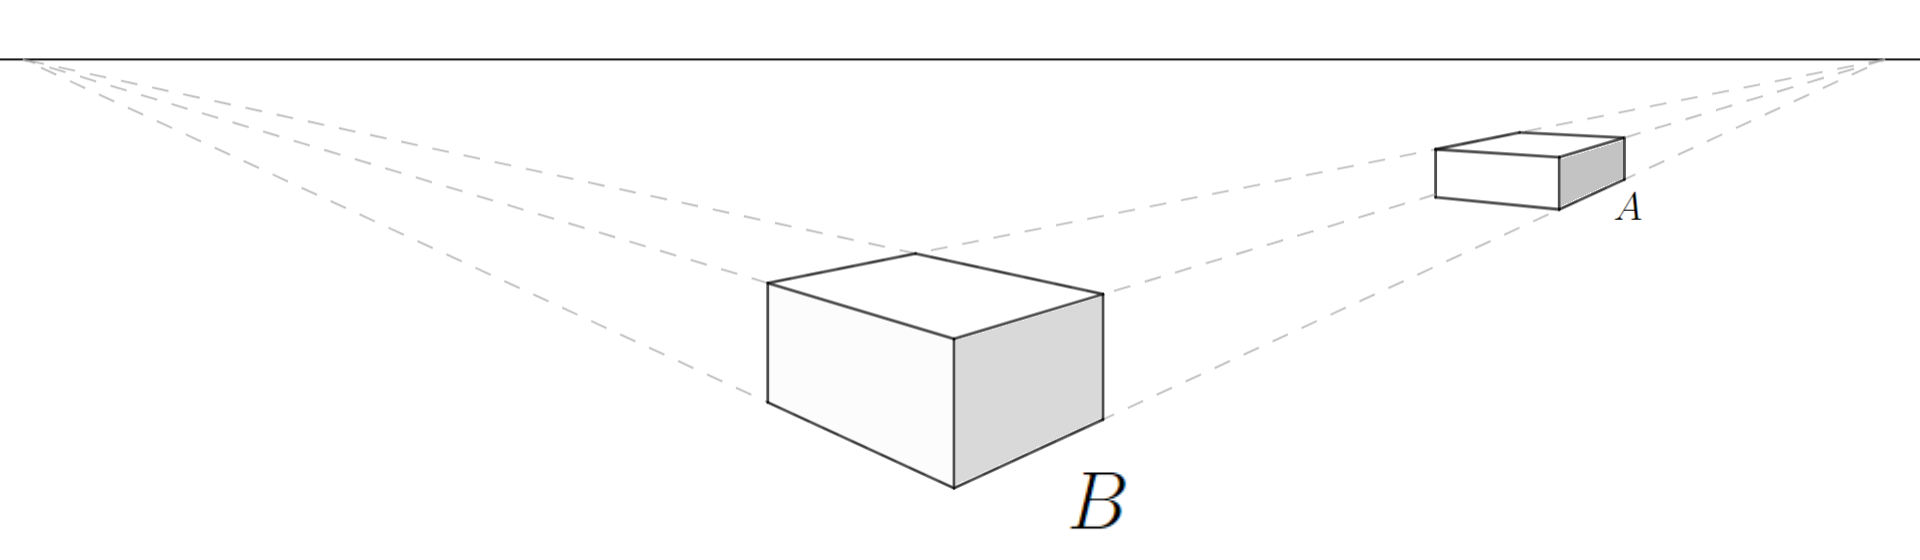
\includegraphics[width=0.6\textwidth]{透视1.png}
    \caption*{\texttt{近大远小}}
\end{figure}

大脑还原事物的形状时,遵循“近大远小”的规律。

同一个物体,离眼睛越远,就显得越小;离眼睛越近,就显得越大。

在平面中,可以使用“近大远小”的方法,表现立体事物的远近。这种表现方法称为\textbf{透视法}。在平面中表现立体形状的技法,
叫做\textbf{作图法},因为传统上,我们用画图的方法来表示现实世界中的立体形状。大部分写实绘画的作图法中都会用到透视法,
让平面中表现的立体景象显得更真实。

透视法有两个基本要诀,一个是“近大远小”,另一个是“向前缩短”。“近大远小”我们已经介绍过了,
“向前缩短”指的是往远方的线并不会真的无限延伸,因此会显得比实际长度短一些。
“向前缩短”可以说是“近大远小”和人的视力有限造成的现象。

\begin{figure}[h] %this figure will be at the right
    % \vspace{4pt}
    \centering
    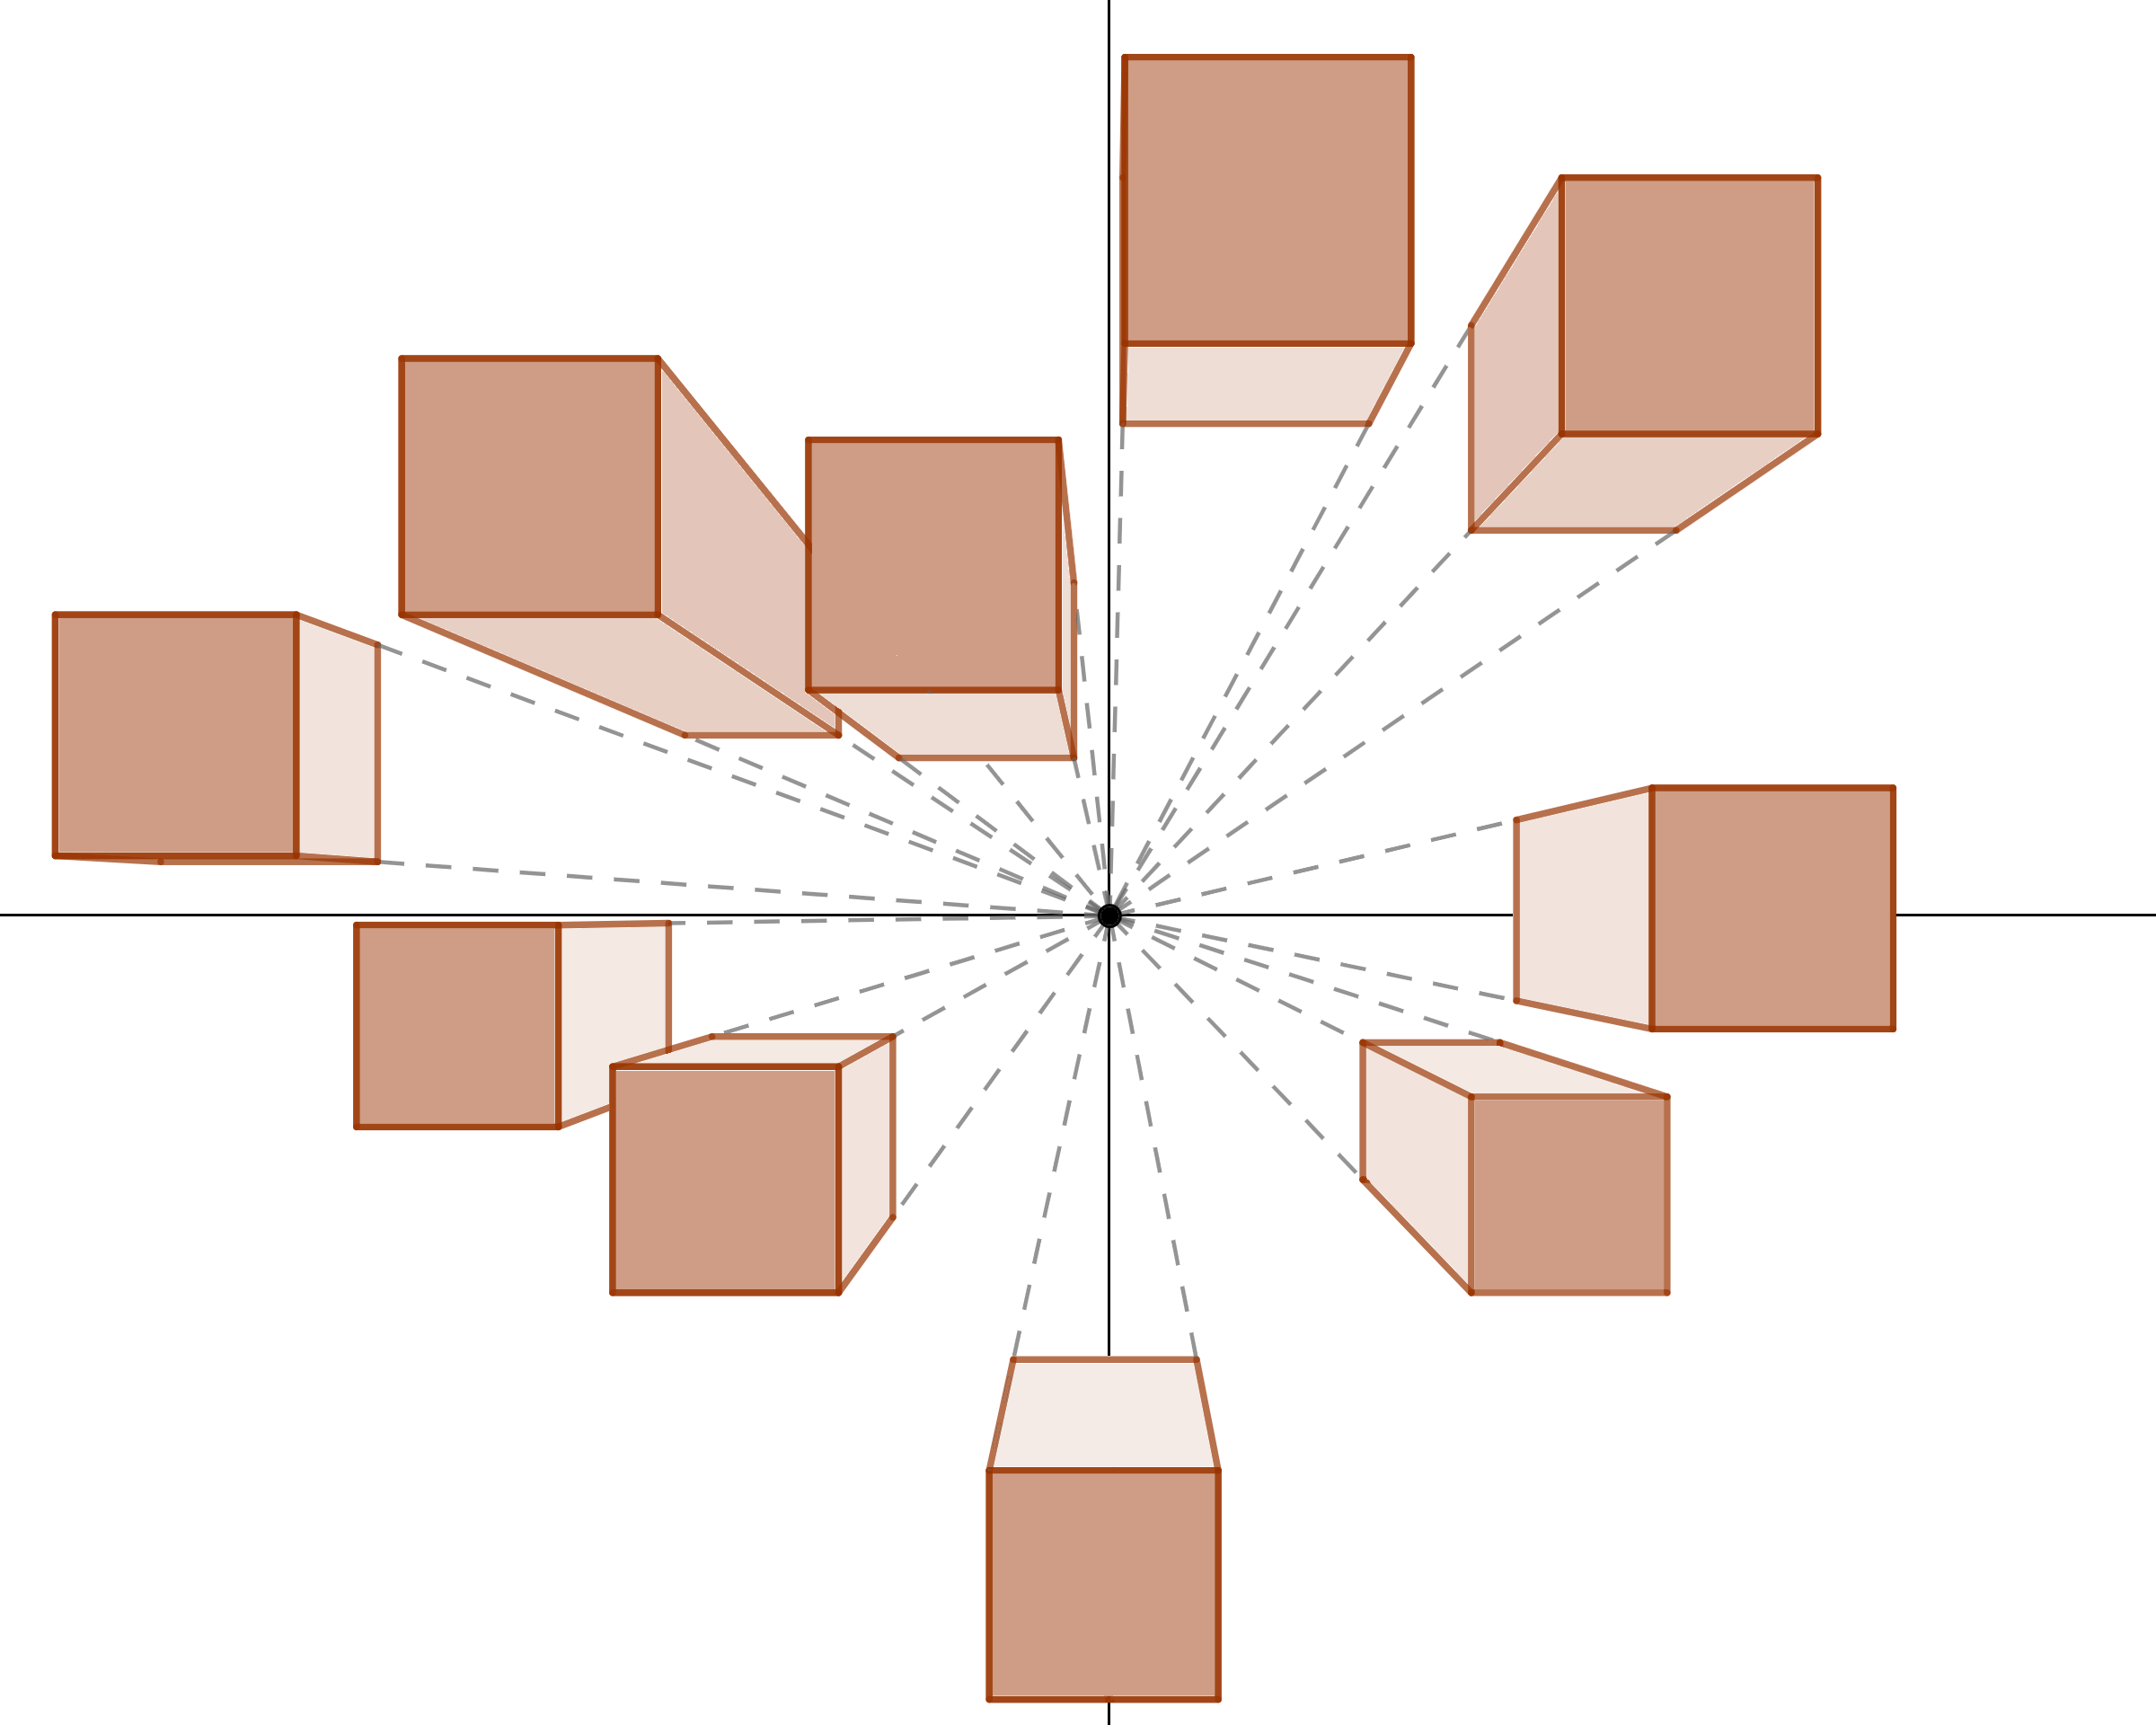
\includegraphics[width=0.6\textwidth]{单点透视.png}
    \caption*{\texttt{单点透视}}
\end{figure}

最简单的透视法是\textbf{直线透视法}。直线透视法认为,现实世界中的平行线,在平面作图时会交于同一点,即便在图中没有相交,其延长线也一定交于同一点。
这个点代表着我们的视力能看到的最远极限,叫做\textbf{灭点}或\textbf{消失点}。灭点可以是一个、两个或三个。
对应的透视法称为单点透视、两点透视和三点透视。

\begin{figure}[h] %this figure will be at the right
    \vspace{-4pt}
    \centering
    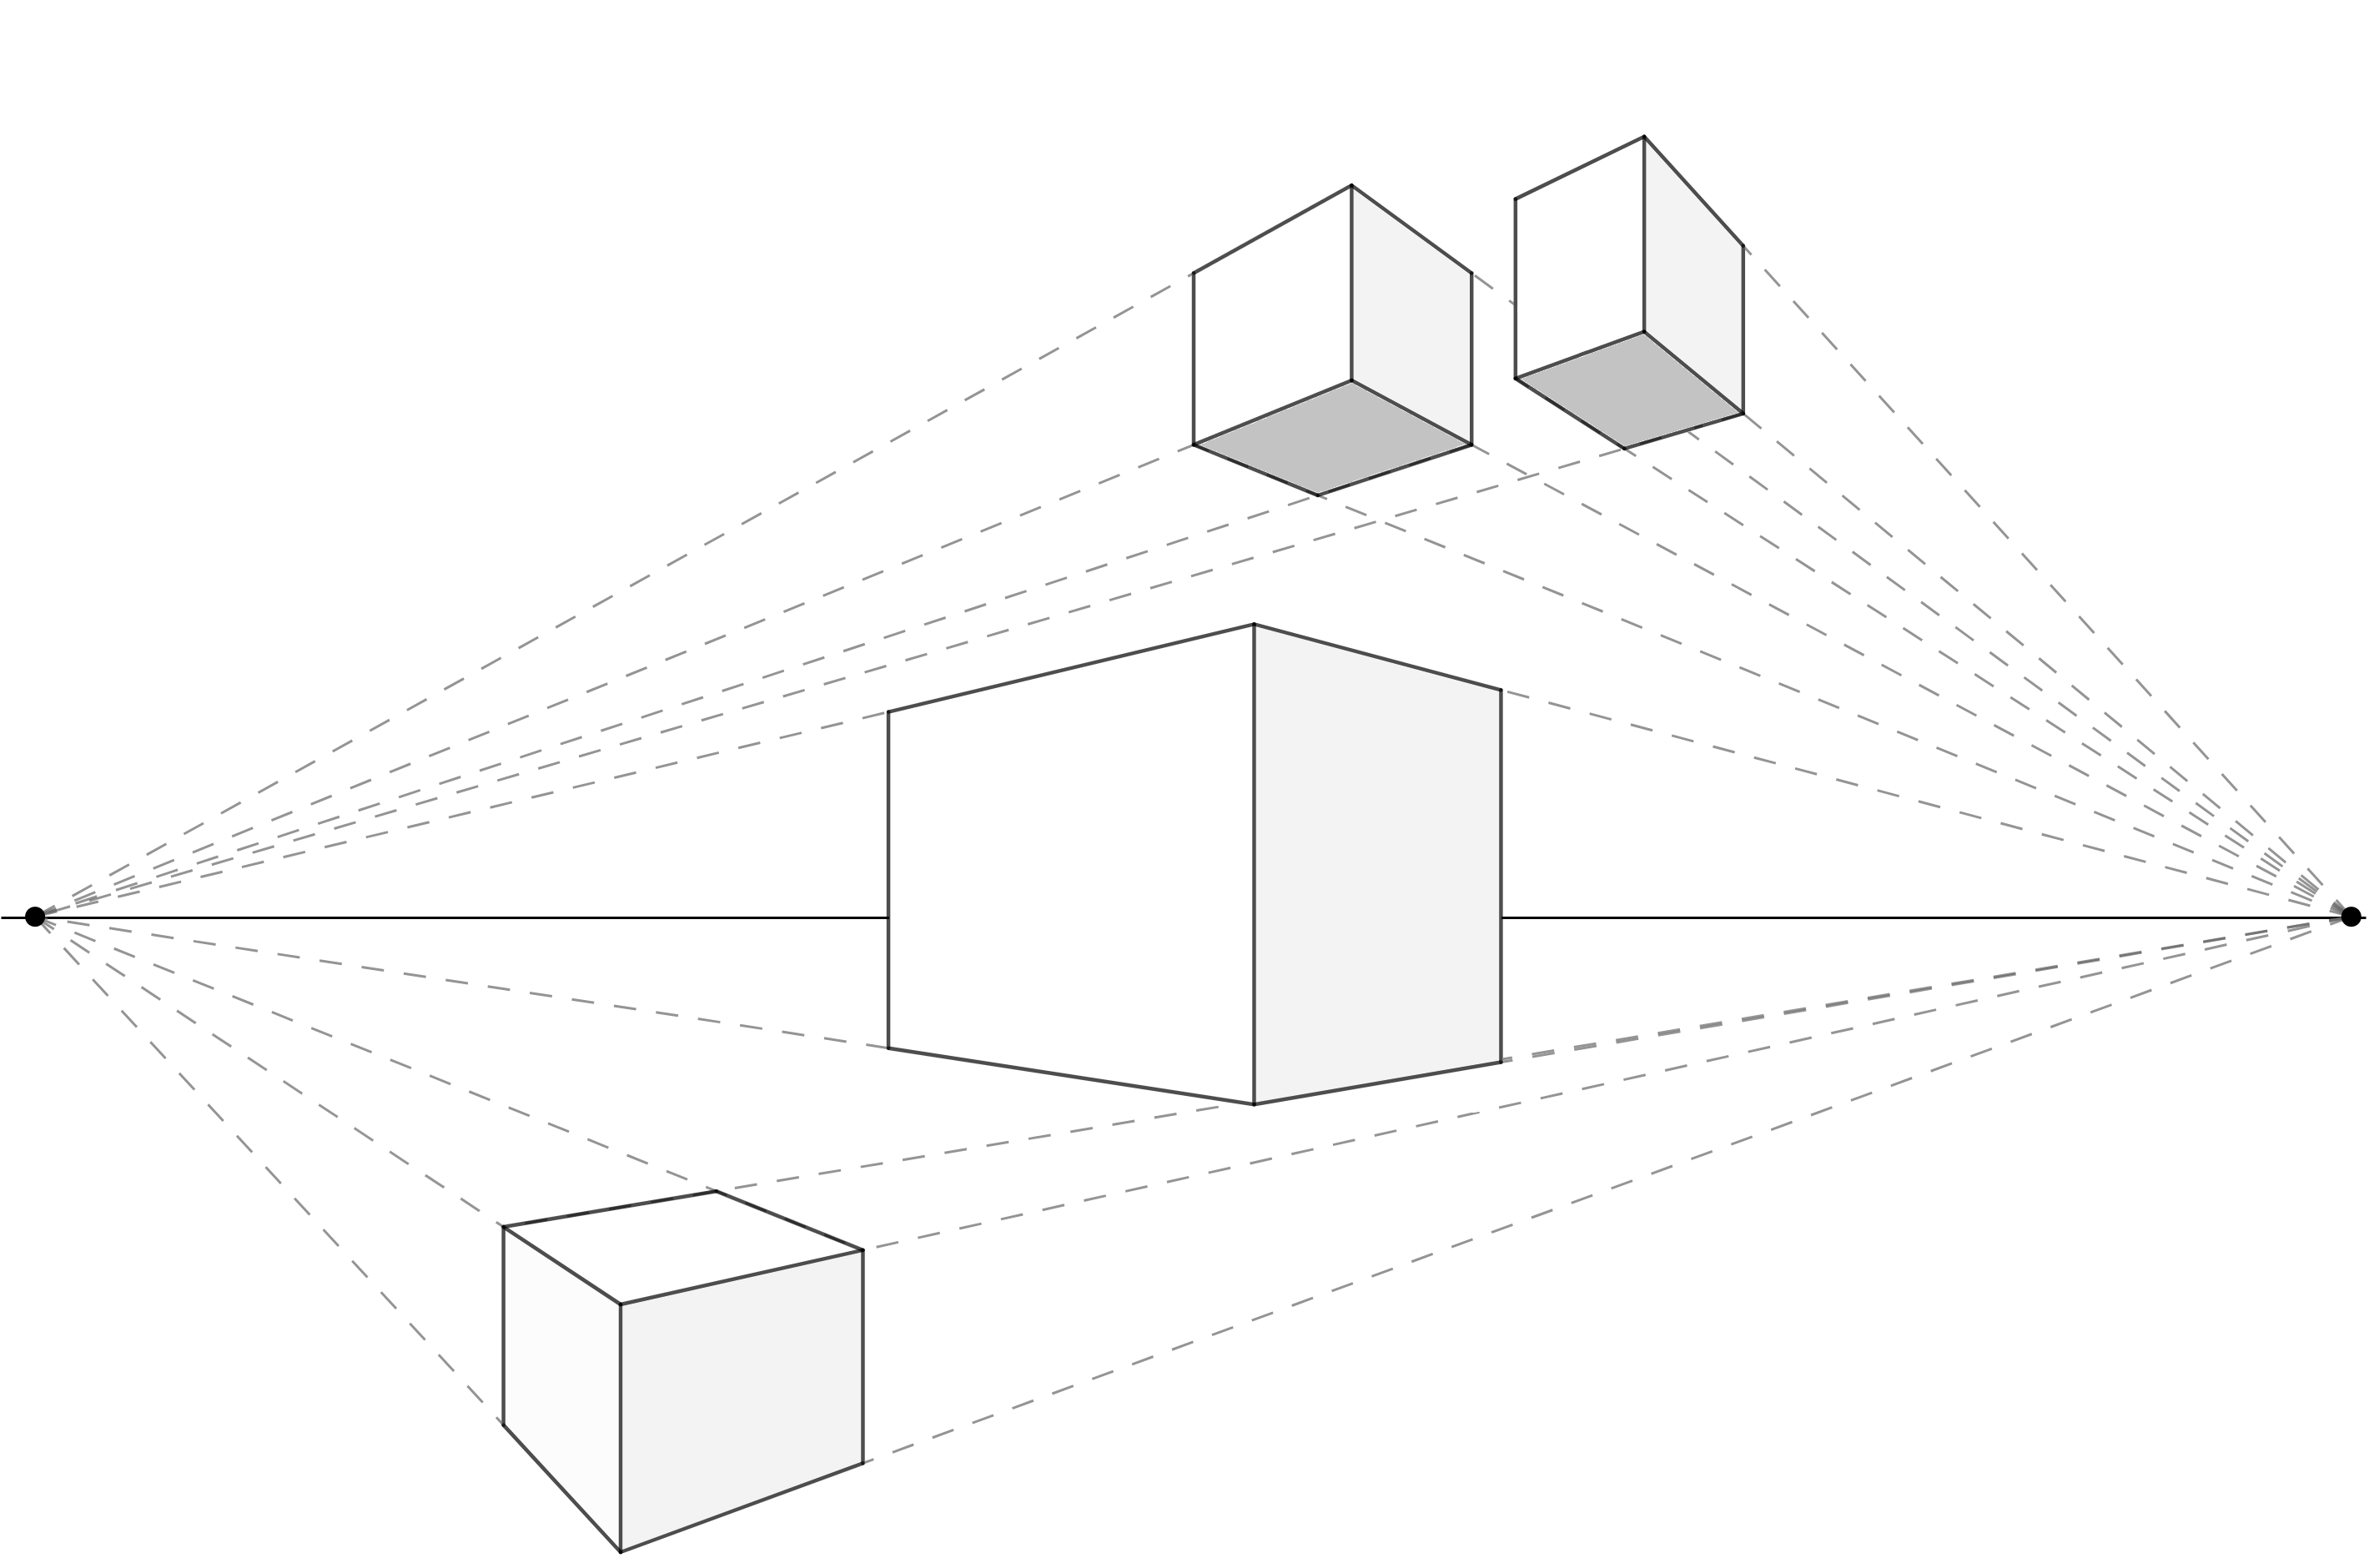
\includegraphics[width=0.6\textwidth]{两点透视.png}
    \caption*{\texttt{两点透视}}
\end{figure}

观察单点透视、两点透视和三点透视的图画,你觉得图中哪些线是现实世界中的平行线?相比现实,它们有什么变化?

\begin{figure}[h] %this figure will be at the right
    \vspace{4pt}
    \centering
    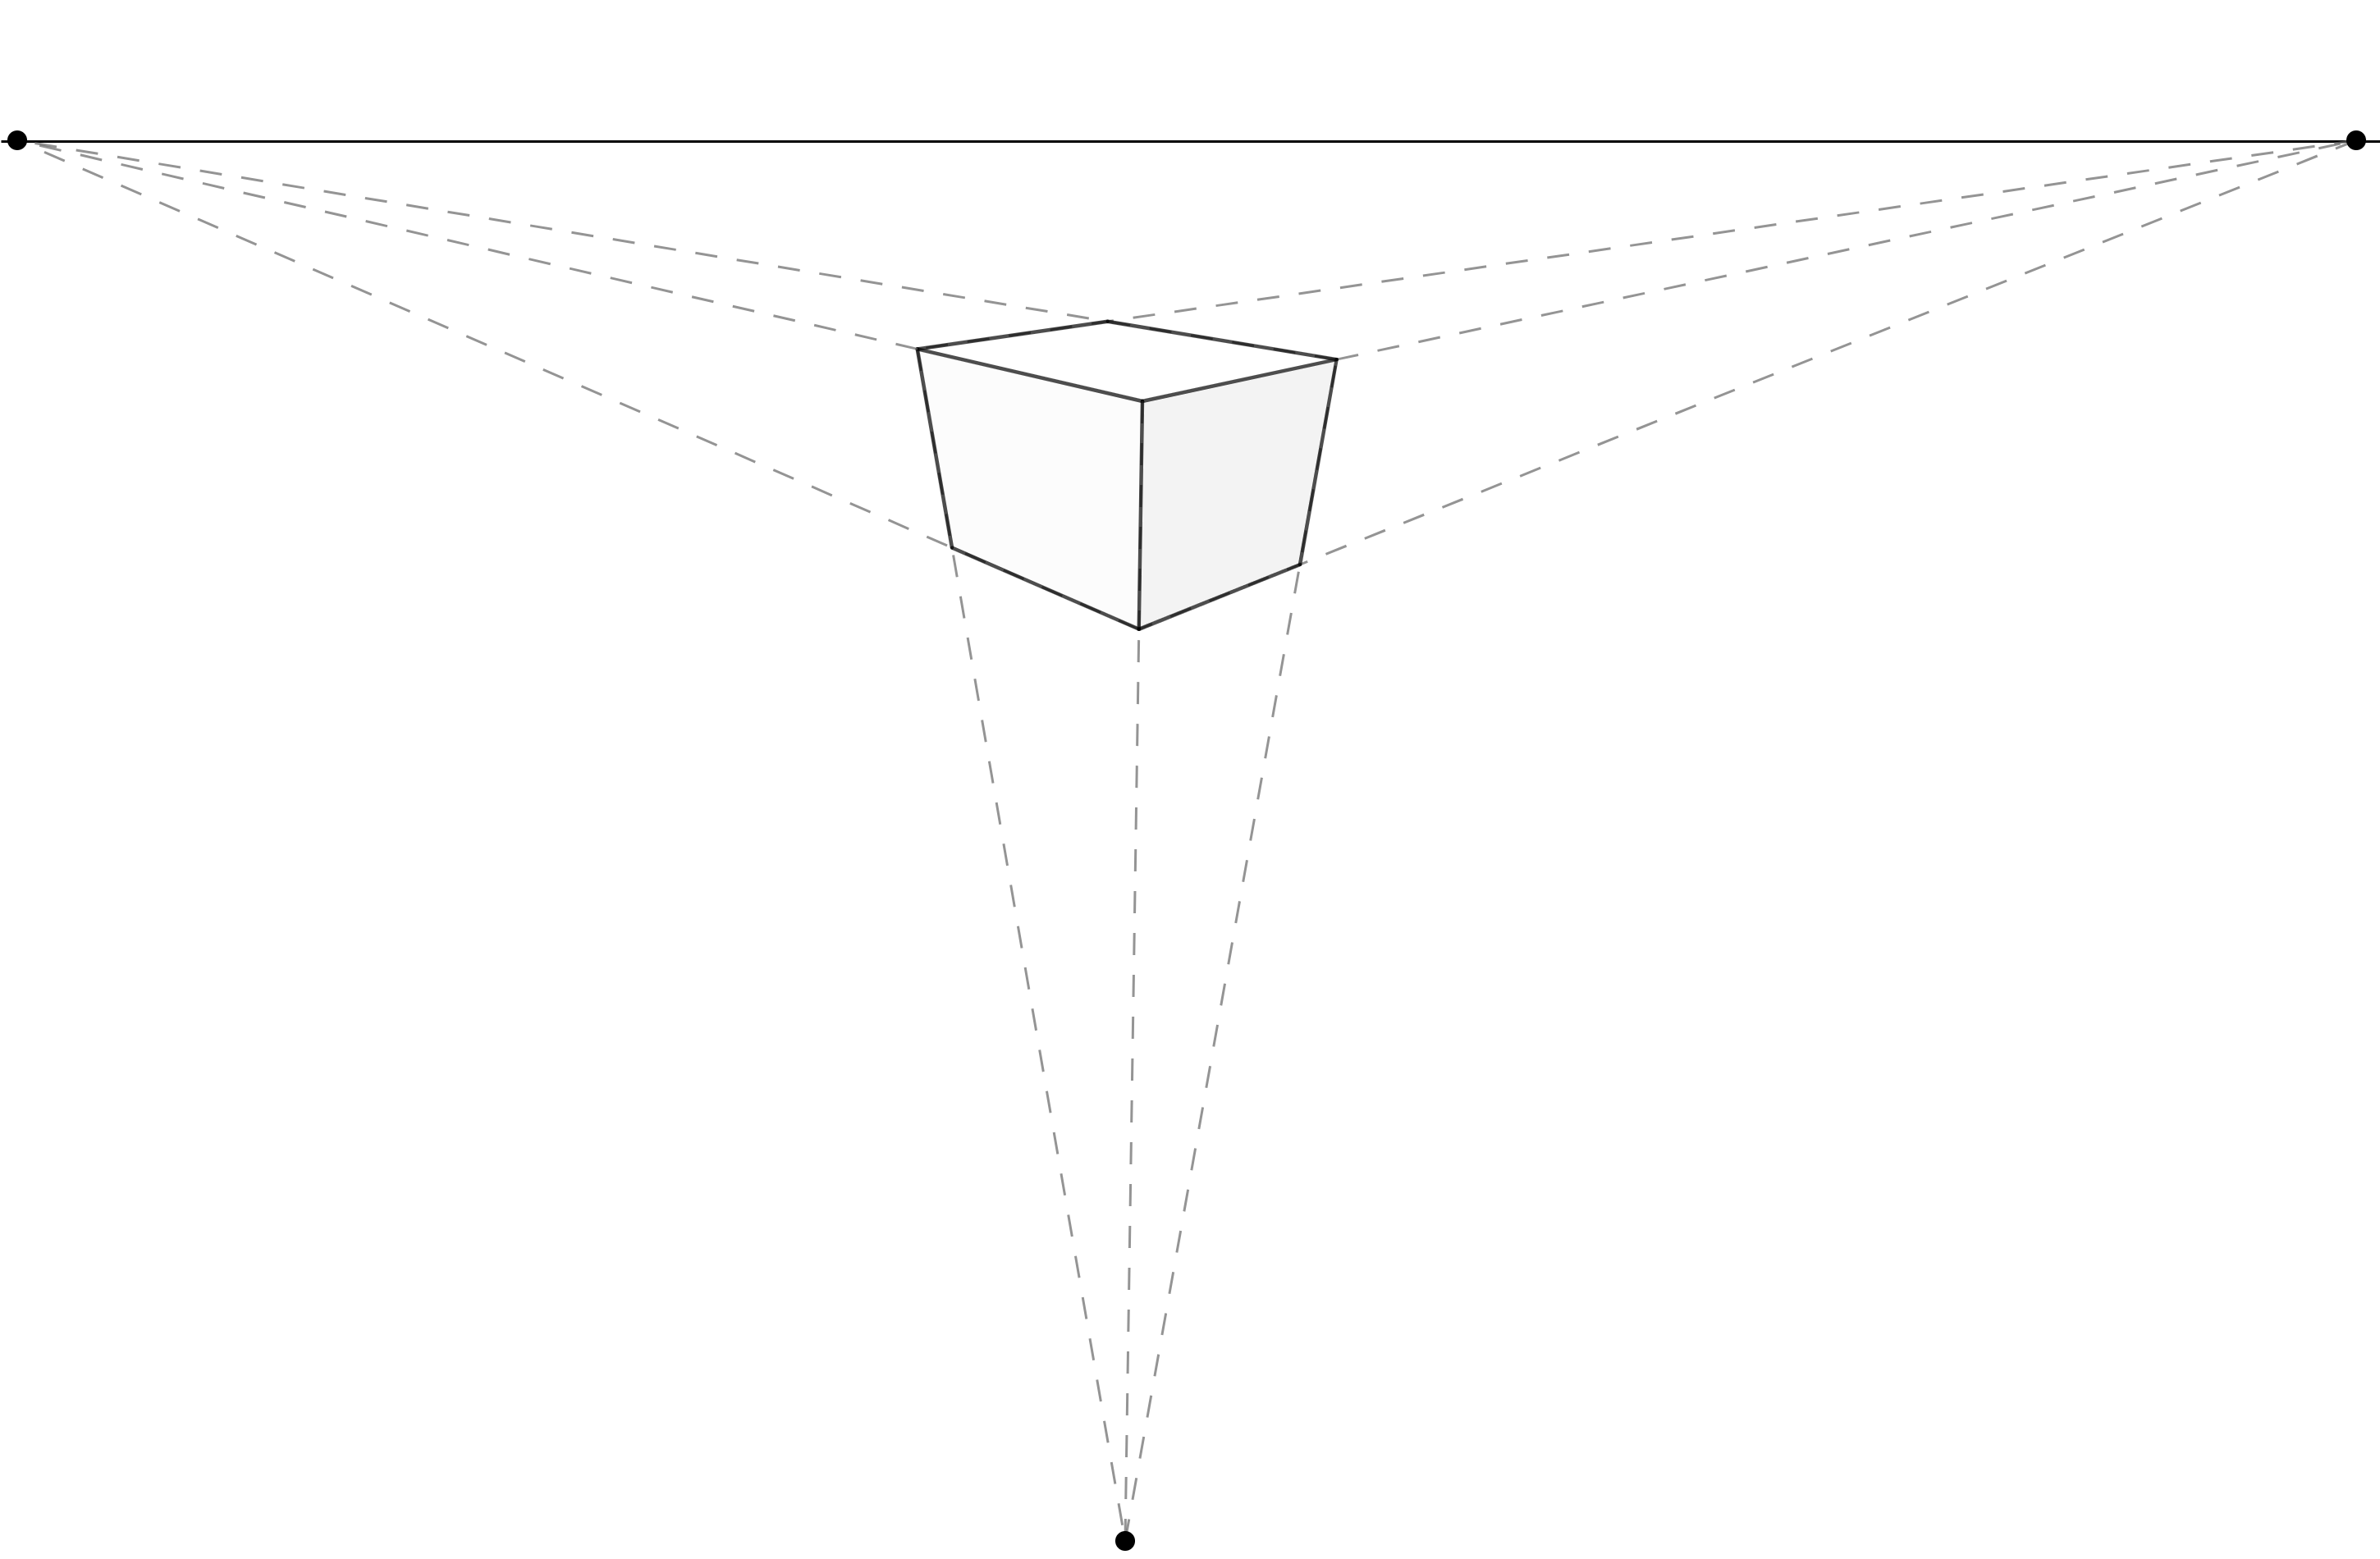
\includegraphics[width=0.6\textwidth]{三点透视.png}
    \caption*{\texttt{三点透视}}
\end{figure}


\begin{sk}
    \mbox{}\\
    \indent 1. 如何理解“近大远小”现象?请试着将学过的知识推广到立体空间中,来解释“近大远小”现象。\\
    \indent 2. 如何理解单点透视、两点透视、三点透视之间的区别和联系?为什么它们都可以反映真实的立体景象?你觉得哪种透视更接近真实?\\
    \indent 3. 你还知道哪些透视法?自行探究并比较各种透视法,它们和以上介绍的透视法有什么不同?
\end{sk}



\chapter{同余}
\begin{ex}\label{ex:3-0-0}
    $7^{65}$的个位数是多少?
\end{ex}
\begin{so}
    从$7^0,7^1,7^2,7^3\cdots$开始找规律。$7^0=1$,$7^1=7$,$7^2=49$,$7^3=343$,$7^4=2401$,$7^5=16807$。
    $7^4$和$7^0$的个位数都是$1$,$7^5$和$7^1$的个位数都是$7$。我们可以总结出这样的规律:个位数是$1$的,乘以$7$得到$7$;
    个位数是$7$的,乘以$7$得到$9$;个位数是$9$的,乘以$7$得到$3$;个位数是$3$的,乘以$7$得到$1$。

    也就是说,如果把$7^0,7^1,7^2,7^3\cdots$的个位数写成一列,应该是这个样子的:
    $$ 1, 7, 9, 3, 1, 7, 9, 3, 1, 7, \cdots$$
    用归纳法不难证明,这列数字以$4$为周期不断重复。所以,要求$7^{65}$的个位数,可以看$65$在相关的周期里处于哪个位置。
    换句话说,只要看$65$除以$4$的余数。$65 = 16 \times 4 + 1$,所以$7^{65}$的个位数和$7^1$的个位数一样,都是$7$。
\end{so}

从这个例子可以看出,两个整数除以同一个数得到相同的余数,是一个重要的性质。我们把这种性质称为\textbf{同余}。
比如,$65$和$1$除以$4$余数都是$1$,我们就说$65$和$1$模$4$同余。$7^{65}$和$7^1$除以$10$余数都是$7$,
我们说$7^{65}$和$7^1$模$10$同余,记为:
$$ 7^{65} \equiv_{10} 7^1 $$

\section{同余类}
整数除以$3$,余数有$0,1,2$三种可能。整数除以$10$,余数有$0,1,\cdots , 9$十种可能。
一般来说,给定正整数$n$,整数除以$n$,余数有$0,1,\cdots , n-1$这$n$种可能。
因此,按除以$n$的余数,可以把整数集分成$n$类。同属一类的数,模$n$同余,所以这$n$类数叫作模$n$\textbf{同余类}。
所有模$n$同余类的集合,叫作模$n$\textbf{同余系}。

每个模$n$同余类,可以写成$\{kn + a \, | \, k\in\mathbb{Z} \}$的形式。也就是说,可以看成某个数$a$不断加上或减去$n$得到的所有数的集合。这个集合是无穷的。不同的模$n$同余类,交集是空集,并集是$\mathbb{Z}$。也就是说,它们是$\mathbb{Z}$的分划。

为了方便,我们从每个模$n$同余类中选一个元素,代表这个同余类。一般来说,可以选$0,1,\cdots,n-1$个数。我们给它们加个上划线,以和作为整数的$0,1,\cdots,n-1$区分:
$$\overline{0},\overline{1},\cdots,\overline{n-1}$$

如果要强调$n$,可以把$n$加在右上角:
$$\overline{0}^n,\overline{1}^n,\cdots,\overline{n-1}^n$$

给定整数$m$,我们可以把它对应到某个模$n$同余类,称为对$n$\textbf{取模}。
比如$n=5$时,$24 \equiv_5 4$,我们把$24$对应到$\overline{4}^5$,
或者说,$24$对$5$取模,得$\overline{4}^5$。

同余关系和相等关系很像,它们是否有一样的性质呢?我们可以验证,同余关系满足以下的性质:
\begin{enumerate}
    \item $\forall \,\, a\in \mathbb{Z}, \quad a \equiv_n a$;
    \item $\forall \,\, a, b \in \mathbb{Z}$,如果$a \equiv_n b$,那么$b \equiv_n a$;
    \item $\forall \,\, a, b \in \mathbb{Z}$,如果$a \equiv_n b$,$b \equiv_n c$,那么$a \equiv_n c$。
\end{enumerate}

满足以上三个性质的二元关系(两个元素之间的关系)称为\textbf{等价关系}。数与数的等于关系是等价关系,数与数的同余关系
也是等价关系。因此,我们可以把同余关系用作同余类之间的等于关系。

整数之间有四则运算,模$n$同余类之间,也可以进行运算。以$n=5$为例子。
我们分别计算$24$和$37$除以$5$的余数,以及它们的和$61$除以$5$的余数:
$$ 24 \equiv_5 4, \,\,\, 37 \equiv_5 2 , \,\,\, 61 \equiv_5 1$$

可以发现:$ 4 + 2 \equiv_5 1$,也就是说,取模和加法可以交换顺序。
可以验证,两个同余类中各取一个元素相加,和所在的同余类,就是两者模$n$余数的和所在的同余类。
用集合的语言,可以写成:
$$\{kn + a + ln + b \, | \, k\in\mathbb{Z}, \, l\in\mathbb{Z} \} = \{kn + a + b \, | \, k\in\mathbb{Z} \}$$

所以,可以定义同余类的加法:
$$ \overline{a} + \overline{b} = \overline{a + b}$$

其中的$\overline{a + b}$指的是$a+b$所在的同余类。为了方便,我们用$a + b$作为代表。

可以验证,同余类的加法也满足结合律和交换律。这里我们只证明同余类的加法满足结合律,交换律的证明留做习题:

\begin{proof2}
    由上可知$ \overline{a} + \overline{b} = \overline{a + b}$,所以
    $$ (\overline{a} + \overline{b}) + \overline{c} = \overline{a + b}+ \overline{c} = \overline{a + b + c}.$$
    类似可得:
    $$ \overline{a} + (\overline{b} + \overline{c}) = \overline{a}+ \overline{b + c} = \overline{a + b + c}.$$
    于是
    $$ \quad \quad \quad (\overline{a} + \overline{b}) + \overline{c}  = \overline{a + b + c} = \overline{a} + (\overline{b} + \overline{c}). \quad \qedhere$$
\end{proof2}

类似可以定义同余类的减法和乘法:
$$ \overline{a} - \overline{b} = \overline{a - b}, \,\,\, \overline{a} \cdot \overline{b} = \overline{a \cdot b}$$

可以验证,同余类的减法性质和整数减法一样,同余类的乘法也满足结合律、交换律和分配律。

能否定义同余类的除法呢?我们来看一个例子。设$n=6$,考虑等式$12 \div 4 = 3$。
$12$、$4$和$3$对$6$取模,得到$0$、$4$和$3$。考虑等式$60 \div 10 = 6$。$60$、$10$和$6$对$6$取模,
得到$0$、$4$和$0$。也就是说,两个模$6$同余类中各取元素相除,商所在的同余类不是唯一的。
所以,我们没法定义模$6$同余类的除法。

再看另一个例子。设$n=5$,考虑以下的“乘法表”:
\begin{center}
    \begin{tabular}{ | p{2em}<{\centering} | p{2em}<{\centering} | p{2em}<{\centering} | p{2em}<{\centering} | p{2em}<{\centering} | p{2em}<{\centering} | }
        \hline
            $\times$   & $\overline{0}$ & $\overline{1}$ & $\overline{2}$ & $\overline{3}$ & $\overline{4}$ \\ [0.5ex] 
        \hline
        $\overline{0}$ & $\overline{0}$ & $\overline{0}$ & $\overline{0}$ & $\overline{0}$ & $\overline{0}$ \\  
        \hline
        $\overline{1}$ & $\overline{0}$ & $\overline{1}$ & $\overline{2}$ & $\overline{3}$ & $\overline{4}$ \\
        \hline
        $\overline{2}$ & $\overline{0}$ & $\overline{2}$ & $\overline{4}$ & $\overline{1}$ & $\overline{3}$ \\
        \hline
        $\overline{3}$ & $\overline{0}$ & $\overline{3}$ & $\overline{1}$ & $\overline{4}$ & $\overline{2}$ \\
        \hline 
        $\overline{4}$ & $\overline{0}$ & $\overline{4}$ & $\overline{3}$ & $\overline{2}$ & $\overline{1}$ \\
        \hline
    \end{tabular}
\end{center}

可以看出,任何模$5$同余类乘以$\overline{0}$都得到$\overline{0}$,非$\overline{0}$同余类乘以不同的同余类,结果也不同。
这说明每个同余类除以另一个同余类(非$\overline{0}$),都必然有唯一的结果。这样我们就定义了模$5$同余系里的除法。

\begin{xt}\label{xt:3-0-0}
    \mbox{}\\
    动手做一做:\\
    \indent 1. 证明同余关系满足等价关系所要求的三个性质。 \\
    \indent 2. 证明同余类的加法满足交换律。 \\
    \indent 3. 证明同余类的减法是加法的逆运算。\\
    \indent 4. 证明同余类的乘法满足结合律和交换律。\\
    \indent 5. 证明同余类的乘法满足分配律。\\
    \indent 6. 证明:如果某模$n$同余类的代表与$n$的最大公因数是$d$,则其中所有元素与$n$的最大公因数都是$d$。\\
    \indent 7. 分别画出模$3$同余系和模$4$同余系的“乘法表”。它们和模$5$同余系的“乘法表”哪些地方相同,哪些地方不同?
\end{xt}

\section{完全同余系和简化同余系}
上一节我们提到模$6$同余系无法定义除法,而模$5$同余系可以定义除法。两者有什么不同呢?
我们画出模$6$同余系的“乘法表”:
\begin{center}
    \begin{tabular}{ | p{2em}<{\centering} | p{2em}<{\centering} | p{2em}<{\centering} | p{2em}<{\centering} | p{2em}<{\centering} | p{2em}<{\centering} | p{2em}<{\centering} | }
        \hline
            $\times$   & $\overline{0}$ & $\overline{1}$ & $\overline{2}$ & $\overline{3}$ & $\overline{4}$ & $\overline{5}$ \\ [0.5ex] 
        \hline
        $\overline{0}$ & $\overline{0}$ & $\overline{0}$ & $\overline{0}$ & $\overline{0}$ & $\overline{0}$ & $\overline{0}$ \\  
        \hline
        $\overline{1}$ & $\overline{0}$ & $\overline{1}$ & $\overline{2}$ & $\overline{3}$ & $\overline{4}$ & $\overline{5}$ \\
        \hline
        $\overline{2}$ & $\overline{0}$ & $\overline{2}$ & $\overline{4}$ & $\overline{0}$ & $\overline{2}$ & $\overline{4}$ \\
        \hline
        $\overline{3}$ & $\overline{0}$ & $\overline{3}$ & $\overline{0}$ & $\overline{3}$ & $\overline{0}$ & $\overline{3}$ \\
        \hline 
        $\overline{4}$ & $\overline{0}$ & $\overline{4}$ & $\overline{2}$ & $\overline{0}$ & $\overline{4}$ & $\overline{2}$ \\
        \hline
        $\overline{5}$ & $\overline{0}$ & $\overline{5}$ & $\overline{4}$ & $\overline{3}$ & $\overline{2}$ & $\overline{1}$ \\
        \hline
    \end{tabular}
\end{center}
可以看到,这个“乘法表”和模$5$同余系的大有不同。同一行或同一列常有重复。
这说明不同的同余类乘同一个同余类得到同一个结果。比如
$$\overline{2}\times \overline{4} = \overline{5}\times \overline{4} = \overline{2}. $$
这就使我们没法定义除法。

如果我们把上面的等式稍作变化,会得到:
$$\overline{0} = (\overline{5} - \overline{2})\times \overline{4} = \overline{3} \times \overline{4}.$$
也就是说,有非$\overline{0}$的同余类相乘等于$\overline{0}$。
同余类乘法的这个性质和整数乘法完全不同。我们把这种非$\overline{0}$同余类叫做\textbf{零因子}。
整数中没有零因子:非$0$的整数相乘必然不是$0$。而只要有这种零因子存在,同余系中就会发生“不同的同余类乘同一个同余类得到同一个结果”的现象,
从而无法定义除法。

有什么办法在模$6$同余系中定义除法呢?我们可以选一部分同余类,在其中定义除法。
如果同余类$\overline{a}$的代表$a$与$6$不互素,设最大公因数是$b$,那么
$$ \frac{a}{b} \times 6 = a \times \frac{6}{b} $$
于是有$\overline{a} \times \overline{\frac{6}{b}} = \overline{0}$,出现零因子。
因此,为了避免零因子问题,我们只选和$6$互素的数所在的同余类,也就是$\overline{1}$和$\overline{5}$。
我们发现$\{\overline{1}, \overline{5}\}$中可以定义乘法和除法(但不再满足加减法)。
\begin{center}
    \begin{tabular}{ | p{2em}<{\centering} | p{2em}<{\centering} | p{2em}<{\centering} | }
        \hline
            $\times$   & $\overline{1}$ & $\overline{5}$ \\ [0.5ex] 
        \hline
        $\overline{1}$ & $\overline{1}$ & $\overline{5}$ \\
        \hline
        $\overline{5}$ & $\overline{5}$ & $\overline{1}$ \\
        \hline
    \end{tabular}
\end{center}
我们把模$6$同余系称为模$6$的\textbf{完全同余系},
把$\{\overline{1}, \overline{5}\}$称为模$6$的\textbf{简化同余系}。

一般来说,我们把模$n$同余系称为模$n$的完全同余系,在其中可以定义加减法和乘法;
把其中所有和$n$互素的同余类的集合称为模$n$的简化同余系
\footnote{通常不把$\overline{0}$计入简化剩余系,以省去讨论除以$\overline{0}$的问题。}。

\begin{tm}\label{tm:3-2-0}
    给定正整数$n$,在模$n$的简化同余系中可以定义乘法和除法。
\end{tm}
\begin{proof2}
    模$n$同余类的乘法已经定义好了。我们只需要说明:简化同余系中的同余类相乘,仍然在简化同余系中。
    这是因为与$n$互素的整数相乘,结果还是与$n$互素。\\
    接下来定义除法。除法是乘法的逆运算。比照数的除法:$a \div b = a \times \frac{1}{b}$。
    因此,只要将简化同余系中每个同余类都对应一个“倒数”,就可以用“乘以倒数”来定义除法。\\
    我们把模$n$简化同余系中的同余类用小于$n$且与$n$互素的正整数来代表,记为
    $$1 = b_1 < b_2 < \cdots < b_{\varphi(n)} = n-1.$$
    其中$\varphi(n)$是模$n$简化同余系的元素个数。考虑任一元素$b_i$,我们接下来会证明:
    $b_ib_1, b_ib_2, \cdots, b_ib_{\varphi(n)}$模$n$两两不同余。
    于是,它们中恰有一个模$n$余$1$。设$b_ib_j \equiv_n 1$,那么$b_j$就是$b_i$的“倒数”。\\
    最后用反证法证明命题:$b_ib_1, b_ib_2, \cdots, b_ib_{\varphi(n)}$模$n$两两不同余。\\
    反设命题不成立,即存在$b_j, b_k$使得$b_ib_j \equiv_n b_ib_k$。这说明$n | b_i(b_j - b_k)$。
    由于$b_i$和$n$互素,根据倍和析因定理,存在整数$p, q$,使得:
    $$ b_ip + nq = 1.$$
    两边乘以$b_j - b_k$,就得到:
    $$ b_i(b_j - b_k)p + nq(b_j - b_k) = b_j - b_k.$$
    等式左边是$n$的倍数,因此$b_j$和$b_k$模$n$同余,这与它们的定义矛盾。\\
    因此命题的否定为假,原命题为真。
\end{proof2}

简化同余系的除法和整数不同,任何同余类都能整除另一个同余类,不需要余数、带余除法的概念。
每个同余类都有自己的“倒数”,比如在模$6$简化同余系中,$\overline{5}\times\overline{5} = \overline{1}$。
我们把同余类的“倒数”称为它的(乘法)\textbf{逆}。

\begin{xt}
    \mbox{}\\
    \indent 1. 写出模$12$的简化同余系。写出$\overline{7}^{12}$的逆。\\
    \indent 2. 比较模$12$简化同余系中的乘除法和模$4$完全同余系中的加减法,它们有何异同?\\
    \indent 3. 写出模$10$的简化同余系。写出$\overline{7}^{10}$的逆。\\
    \indent 4. 比较模$10$简化同余系中的乘除法和模$4$完全同余系中的加减法,它们有何异同?\\
    \indent 5. 给定素数$n$,写出模$n$简化同余系。
\end{xt}

\section{方余定理}
与模$n$简化同余系密切相关的一个定理是方余定理\footnote{这个定理也称为欧拉定理。但以欧拉命名的定理太多了。为了避免混淆,这里不采用。}。
\begin{tm}{\textbf{方余定理} }\label{tm:3-3-0}
    设$a$是模$n$简化同余系中某个同余类中的元素,则:
    $$ a^{\varphi(n)} \equiv_n 1 $$
    其中$\varphi(n)$是模$n$简化同余系中同余类的个数。
\end{tm}
比如,模$10$简化同余系有$4$个元素:$\overline{1}, \overline{3},\overline{7},\overline{9}$。
$7$属于同余类$\overline{7}$,则$7^4 \equiv_{10} 1$。

\begin{proof2}
    我们把模$n$简化同余系中的同余类用小于$n$且与$n$互素的正整数来代表,记为
    $$1 = b_1 < b_2 < \cdots < b_{\varphi(n)} = n-1.$$
    它们两两不同余。把它们各自乘以$a$,得到$\varphi(n)$个整数:$ab_1, ab_2, \cdots , ab_{\varphi(n)}$。
    前面我们已经证明了,它们仍然两两不同余。\\
    这说明这$\varphi(n)$个整数也分别代表模$n$简化同余系中的各个同余类。\\
    考虑乘积:$b_1 b_2 \cdots b_{\varphi(n)}$。$(ab_1) (ab_2) \cdots (ab_{\varphi(n)})$和它同余。
    也就是说:
    $$b_1 b_2 \cdots b_{\varphi(n)} \equiv_n (ab_1) (ab_2) \cdots (ab_{\varphi(n)}) \equiv_n a^{\varphi(n)} b_1 b_2 \cdots b_{\varphi(n)}.$$
    由于$b_1 b_2 \cdots b_{\varphi(n)}$也与$n$互素,我们把等式两边除以$b_1 b_2 \cdots b_{\varphi(n)}$,就得到:
    $$ a^{\varphi(n)} \equiv_n 1 . $$
\end{proof2}

如果$n$是素数,那么$1,2, \cdots , n-1$都和它互素,
于是模$n$的简化同余系就是$\{\overline{1},\overline{2}, \cdots , \overline{n-1}\}$,$\varphi(n) = n-1$。
根据方余定理,只要$a$不是$n$的倍数,就有:
$$ a^{n-1} \equiv_n 1 .$$
这个结论也叫做费马小定理。

\begin{xt}\label{xt:3-3-0}
    \mbox{}\\
    给定素数$n$,证明:\\
    \indent 1. 除了$\overline{1}$和$\overline{n-1}$,其它同余类的逆都不是自己。\\
    \indent 2. $(n-1)! \equiv_n -1.$ \\
    设$a$与$n$互素,称使得$a^m \equiv_n 1$的最小正整数$m$为$a$模$n$的\textbf{阶}。\\
    \indent 3. 证明$a$的阶整除$\varphi(n)$。\\
    \indent 4. 如果$a$的阶等于$\varphi(n)$,就说$a$是模$n$的\textbf{原根}。证明:如果$a$是模$n$的原根,
    那么模$n$简化同余系可以写成:$\{\overline{a^0}, \overline{a^1}, \cdots , \overline{a^{\varphi(n)-1}}\}$。\\
    \indent 5. 找出所有模$7$的原根。
\end{xt}

\chapter{用数据说话}
数据是客观事物的定量记录。比如,以下列表中有某班级学生的身高数据。

\begin{center}
    \begin{tabular}{ p{4em}<{\centering} !{\color{white} \vrule width 2pt} p{3em}<{\centering} !{\color{white} \vrule width 2pt} p{6em}<{\centering} }
        \rowcolor{gd} \textbf{姓名} & \textbf{学号} & \textbf{身高(厘米)} \\ [0.5ex] 
        \noalign{{\color{white}\hrule height 2pt}} % \hline\hline
        \rowcolor{gl} 张三 & $214092$ & $166.4$ \\  
        \noalign{{\color{white}\hrule height 2pt}}% \hline
        \rowcolor{gd} 李四 & $214033$ & $171.5$ \\  
        \noalign{{\color{white}\hrule height 2pt}}% \hline
        \rowcolor{gl} 王五 & $210819$ & $164.8$ \\  
        \noalign{{\color{white}\hrule height 2pt}}% \hline
        \rowcolor{gd} $\vdots$ & $\vdots$ & $\vdots$ \\  
    \end{tabular}
\end{center}

生产生活中,我们常常以数量等形式记录客观事物的特征和属性。
以合理的方式组织、呈现的数据,能帮助我们了解事物的本质,成为我们讨论、判断、决策的依据。

数据一般由\textbf{义}和\textbf{值}两部分构成。比如,我国2020年国民生产总值为101兆5986亿元人民币。
这个数据的义是“我国2020年国民生产总值”,值是“101兆5986亿元人民币”。
数据的义和值缺一不可。没有义,就无法理解数据代表什么、与什么事物有关;没有值,就无法使用数据来了解相关事物。

\section{样本和特征}
要了解事物的某种性质,我们需要收集数据。比如,要了解学生的身体素质,我们可以通过体检收集学生的身高、体重、肺活量、血压等相关数据。
如果我们要了解学生的身高,就要从每个学生的身高数据出发进行研究。这里每个学生的身高称为一份\textbf{样本}。对学生的各项数据来说,
和某种性质相关的某一项,称为一个\textbf{特征}。比如,我们收集了$100$名学生的身高、体重、肺活量和血压数据。
从总体来说,每个学生的数据是一个样本,共有$100$份样本。每个学生的数据都包括身高、体重、肺活量、血压。因此,这$100$份样本涉及$4$个特征。
如果我们只研究学生的身高状况,那么可以把每个学生的身高数据看作一份样本。


\begin{wrapfigure}[10]{r}{0.29\textwidth} %this figure will be at the left
    \vspace{-20pt}
    \flushright
    
\includegraphics[width=0.27\textwidth]{问卷调查2.png}
\end{wrapfigure}

实际生活中,收集数据样本的方式多种多样。一种常见的方式是通过调查问卷获得数据。右图是一份关于电视剧的调查问卷(部分)。

利用调查问卷,可以收集人们的主观想法、喜好。如果要收集事物的客观性质,更多是通过科技手段。

直接收集到的数据,也许无法直接反映事物的本质,难以让我们总结事物的规律。
为此,我们对收集到的数据进行整理加工,得到新的数据。
为了区别直接收集到的数据和经过人为整理加工的数据,我们一般把前者称为\textbf{原始数据},把后者称为\textbf{生成数据}。

通常来说,整理加工数据的手段主要有以下几种:提高数据质量、转化数据形态、变换数据结构、新造特征。

为了提高数据质量而加工数据,称为数据清洗。我们收集到的数据,往往并不是我们理想中的样子。比如,我们收集$100$名学生的身高、体重、肺活量、血压数据,
结果中可能有$3$名学生的血压数据缺失,$6$名学生的肺活量明显错误,$4$名学生的数据重复记录,$7$名学生的身高与上次体检结果严重不一致等情况。
这些问题会影响我们研究数据,作出结论。因此,需要清洗数据,提高数据质量,以便接下来进行研究。

检查数据质量,通常从以下几个方向入手:\textbf{完整性}、\textbf{唯一性}、\textbf{一致性}、\textbf{正确性}。
\begin{itemize}
    \item 完整性检查,就是检查数据是否有缺失的。比如,收集$20$个城市的就业率做研究,结果缺了某城市的数据,则数据不完整。
    \item 唯一性检查,就是检查不同途径、时间收集的数据是否有重复的。比如,收集学生对新游泳馆的评价,出现同一名学生的两份样本,说明数据重复了。
    \item 一致性检查,就是检查有关系的数据是否一致、是否合理。比如,收集市场的交易数据,各账户买入和卖出的数量分别相加,得到的总买入量应该等于总卖出量。
    如果总买入量和总卖出量不相等,则数据不一致。
    \item 正确性检查,就是核实数据是否正确无误。比如,收集学生的身高数据,出现某学生身高$173$米,说明数据有误。
\end{itemize}
不同的研究中,出于实际需要和综合考虑,会使用不同的手段清洗数据,处理数据的完整性、一致性、唯一性、正确性问题。

转化数据形态,就是把数据的值用另一种形式呈现。转化数据形态往往是为了从另一个角度看待数据的值。
比如,收集$100$名学生的肺活量:
\begin{center}
    \begin{tabular}{ p{3em}<{\centering} !{\color{white} \vrule width 2pt} p{7em}<{\centering} }
        \rowcolor{gd} \textbf{姓名} & \textbf{肺活量(毫升)} \\ [0.5ex] 
        \noalign{{\color{white}\hrule height 2pt}} % \hline\hline
        \rowcolor{gl} 张三 & 2800 \\  
        \noalign{{\color{white}\hrule height 2pt}}% \hline
        \rowcolor{gd} 李四 & 3200 \\
        \noalign{{\color{white}\hrule height 2pt}}% \hline
        \rowcolor{gl} 王五 & 4100 \\  
        \noalign{{\color{white}\hrule height 2pt}}% \hline
        \rowcolor{gd} $\vdots$ & $\vdots$ \\  
        \noalign{{\color{white}\hrule height 2pt}}% \hline
        \rowcolor{gl} 钱六 & 3850 \\
    \end{tabular}
\end{center}

我们可以把数据转为:
% 按1000ml分箱
\begin{center}
    \begin{tabular}{ p{3em}<{\centering} !{\color{white} \vrule width 2pt} p{3em}<{\centering} !{\color{white} \vrule width 2pt} p{3em}<{\centering}!{\color{white} \vrule width 2pt} p{3em}<{\centering}!{\color{white} \vrule width 2pt} p{3em}<{\centering}!{\color{white} \vrule width 2pt} p{3em}<{\centering}!{\color{white} \vrule width 2pt} p{3em}<{\centering} }
        \rowcolor{gd} \textbf{姓名} & $[0,\,\, 1)$ & $[1,\,\, 2)$ & $[2,\,\, 3)$ & $[3,\,\, 4)$ & $[4,\,\, 5)$ & $> 5$ \\ [0.5ex] 
        \noalign{{\color{white}\hrule height 2pt}} % \hline\hline
        \rowcolor{gl} 张三 & $0$ & $0$ & $1$ & $0$ & $0$ & $0$  \\  
        \noalign{{\color{white}\hrule height 2pt}}% \hline
        \rowcolor{gd} 李四 & $0$ & $0$ & $0$ & $1$ & $0$ & $0$  \\
        \noalign{{\color{white}\hrule height 2pt}}% \hline
        \rowcolor{gl} 王五 & $0$ & $0$ & $0$ & $0$ & $1$ & $0$  \\
        \noalign{{\color{white}\hrule height 2pt}}% \hline
        \rowcolor{gd} $\vdots$ & $\vdots$ & $\vdots$ & $\vdots$ & $\vdots$ & $\vdots$ & $\vdots$ \\  
        \noalign{{\color{white}\hrule height 2pt}}% \hline
        \rowcolor{gl} 钱六 & $0$ & $0$ & $0$ & $1$ & $0$ & $0$  \\
    \end{tabular}
\end{center}

我们以升为单位,把肺活量的范围分划为几个区间,每个人的肺活量的值落在哪个区间,就在对应的列记$1$,其他列记$0$。
这让我们用另一种角度来观察肺活量数据。

变换数据结构,是指用另一种方式组织数据。原始数据不容易理解,可能是因为数据组织的方式不合其义。
组织数据的方式越符合其义,我们就越容易通过数据理解事物的本质。
比如,我们收集某些影视演员的出演影视作品的数据,研究演员之间的关系。原始数据是各个演员的作品列表:
% 演员作品表
\begin{center}
    \begin{tabular}{ p{4em}<{\centering} !{\color{white} \vrule width 2pt} p{22em}<{\centering} }
        \rowcolor{gd} \textbf{姓名} & \textbf{作品} \\ [0.5ex] 
        \noalign{{\color{white}\hrule height 2pt}} % \hline\hline
        \rowcolor{gl} 周比利 & 《少年陈真》、《精武英雄》、《鼠胆龙威》、…… \\  
        \noalign{{\color{white}\hrule height 2pt}}% \hline
        \rowcolor{gd} 斯琴高娃 & 《北京爱情故事》、《骆驼祥子》、《香魂女》、 …… \\  
        \noalign{{\color{white}\hrule height 2pt}}% \hline
        \rowcolor{gl} 朱咪咪 & 《百变星君》、《审死官》、《唐伯虎点秋香》、…… \\  
        \noalign{{\color{white}\hrule height 2pt}}% \hline
        \rowcolor{gd} $\vdots$ & $\vdots$ \\  
        \noalign{{\color{white}\hrule height 2pt}}% \hline
        \rowcolor{gl} 李绮虹 & 《西贡的童话》、《爱未央》、《圣诞玫瑰》、…… \\  
        \noalign{{\color{white}\hrule height 2pt}}% \hline
        \rowcolor{gd} 张涵予 & 《风声》、《智取威虎山》、《红海行动》、…… \\  
    \end{tabular}
\end{center}

我们可以根据共演关系,把数据结构改为下图。每个圆点代表一个演员。曾经共演的演员之间连线,否则不连线。
% 演员关系图
\begin{figure}[H] %this figure will be at the right
    \vspace{8pt}
    \centering
    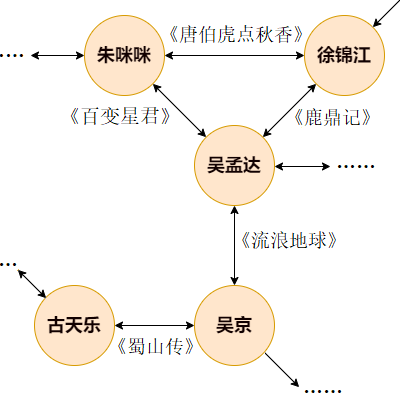
\includegraphics[width=0.3\textwidth]{演员关系图1.png}
\end{figure}

从图中我们能够看出不同演员之间的合作关系。我们也可以把共演关系用数表的方式呈现。曾经共演的演员,
相应的格子中填入共演作品数目,否则填$0$:
% 相关矩阵
\begin{center}
    \begin{tabular}{ | p{3.2em}<{\centering} | p{3.2em}<{\centering} | p{3.2em}<{\centering} | p{3.2em}<{\centering} | p{3.2em}<{\centering} | p{2em}<{\centering} | }
        \hline
           & 朱咪咪 & 吴孟达 & 古天乐 & 吴京 & $\cdots$ \\ [0.5ex]
        \hline
        朱咪咪 & - & $3$ & $0$ & $0$ & $\cdots$ \\  
        \hline
        吴孟达 & $3$ & - & $3$ & $1$ & $\cdots$ \\  
        \hline
        古天乐 & $0$ & $3$ & - & $4$ & $\cdots$ \\ 
        \hline
        吴京 & $0$ & $1$ & $4$ & - & $\cdots$ \\ 
        \hline
        $\vdots$ & $\vdots$ & $\vdots$ & $\vdots$ & $\vdots$ &  \\  
        \hline
    \end{tabular}
\end{center}

新造特征,就是从原始数据的某些特征出发,构造新的数据。
比如,从身高和体重数据出发,用体重除以身高的平方,就得到新特征:体质指数。

% \begin{xt}
%     1. 
% \end{xt}

\section{描述和分析}
上一节的例子中,我们收集了$100$名学生的身高、体重、肺活量、血压数据。如何通过这些数据,了解这些学生的身体素质情况呢?
我们可以查看每个学生的数据。然而,人的认知和理解能力是有限的。我们无法直接把这$400$个数值直接反映在头脑中。
为此,我们希望用更少的信息来描述这些数据,让我们对这些数据有大概的认识。这种手段叫作\textbf{描述统计}。
描述统计中最基本的方式,是从数据出发算得一个数量,来描述数据。我们把这样的数量称为\textbf{统计量}。以下是一些常见的统计量。

\textbf{极值}:某特征所有样本值中最大的,称为该特征的\textbf{极大值};所有样本值中最小的,称为该特征的\textbf{极小值}。
比如,我们可以查看所有学生的体重,找出其中最大的值和最小的值。

\textbf{平均数}:某特征所有样本值之和,除以样本的个数,称为该特征的平均数或均值。
比如,我们把所有学生的身高值加起来,除以$100$,就得到学生平均身高。

\textbf{中位数}:如果某个数值比某特征一半样本的值大,比另一半样本的值小,就说它是该特征的中位数。
显然,这个定义是不严谨的,实际计算时需要严谨的定义。最简单也是最常用的定义是:
将该特征所有样本的值从小到大排列。如果样本个数$N$是奇数:$N = 2n + 1$,那么取第$n+1$大的数为中位数;如果样本个数是偶数:$N=2n$,
那么取第$n$大和第$n+1$大的数的均值为中位数。
比如,把$100$名学生的肺活量值从小到大排列,第$50$大的值和第$51$大的值之和除以$2$,就是中位数。

根据极值、平均数和中位数,我们可以大致描述数据的总体情况。比如,知道了学生的身高极小值是$144$厘米,极大值是$191$厘米,
平均值是$165.7$厘米,中位数是$163.8$厘米,我们就对这$100$名学生的身高有了基本的认识。

要更进一步分析数据,可以通过\textbf{分位数}和\textbf{直方图}。

分位数是中位数概念的推广。可以想象把所有样本的值标记在数轴上,
用手指从左边第一个值起,往右划过去,数过一个又一个值。数过一半样本时的值,大致就是中位数。
类似地,设有$0 < q < 1$,数过的样本数量和总数量之比为$q$的时候,指向的值就可以称为样本的$q$\textbf{分位数}。
$q$称为分位,一般用百分数表示。中位数就是$50\%$分位数。

显然,从右往左数也可以定义一种分位数。我们把从左往右数得到的称为\textbf{左}$q$\textbf{分位数}或\textbf{下}$q$\textbf{分位数},
把从右往左数得到的称为\textbf{右}$q$\textbf{分位数}或\textbf{上}$q$\textbf{分位数}。

分位数和中位数一样,是一种模糊的说法。实际计算中,我们要采用更严谨的定义。

给定$N$个样本值$x_1 \leqslant x_2  \leqslant  \cdots  \leqslant x_N$和某个值$a$,
定义$n^{-}$为小于等于$a$的样本个数。
数轴上,$a$从$x_1 - 1$向$x_N + 1$运动时,$n^-$从$0$增大到$N$。
$a$从某个$x_i$离开,运动到$x_{i+1}$期间,$n^-$是不变的。$a$到达$x_{i+1}$时,$n^-$增大。

分位数的自然定义:
如果$a$到达某个$x_{i}$前,$n^- < qN$,而到达$x_{i}$时$n^- \geqslant qN$,就定义$x_{i}$为左$q$分位数。
如果在某段$x_i$到$x_{i+1}$期间$n^- = qN$,就定义$(1 - q)x_{i} + qx_{i+1}$为左$q$分位数。

此外还可以定义顺分位数。区别在于,如果在某段$x_i$到$x_{i+1}$期间$n^- = qN$,
顺分位数仍定义左端$x_i$为左$q$分位数。

自然定义的分位数和之前中位数的定义相洽,顺分位数则更方便计算。

分位数按照样本的数量来划分样本,划分越细,越有利于我们了解样本的分布情况。
比如,根据$100$个学生的身高,求得分位数如下:
\begin{center}
    \begin{tabular}{ | p{3.8em}<{\centering} | p{2em}<{\centering} | p{2em}<{\centering} | p{2em}<{\centering} | p{2em}<{\centering} | p{2em}<{\centering} | p{2em}<{\centering} | p{2em}<{\centering} | p{2em}<{\centering} | p{2em}<{\centering} | }
        \hline
            $q$   & $10\%$ & $20\%$ & $30\%$& $40\%$& $50\%$& $60\%$& $70\%$& $80\%$& $90\%$ \\ [0.5ex] 
        \hline
        {\scriptsize 分位数(cm)} & $149.7$ & $154.3$ & $158.0$ & $161.2$ & $163.8$ & $167.5$ & $171.7$ & $175.6$ & $180.2$ \\  
        \hline
    \end{tabular}
\end{center}

可以看出,学生身高在$40\%$到$50\%$阶段较为集中,在$80\%$到$90\%$阶段较为稀疏。

% 144 148.7 153.4 158.1 162.8 167.5 172.2 176.9 181.6 186.3 191

直方图是另一种展示样本分布情况的方法。我们取定某个包含了所有样本值的区间,然后将其均匀分划为若干份。
比如,我们取学生身高的极小值和极大值构建区间$[144, \,\,191]$,将其均匀划分成$10$份,每份长为$\frac{191-144}{10}=4.7$。
数轴上,左起第一个区间是$[144, \,\,148.7)$,第二个区间是$[148.7, \,\,153.4)$,等等。最右边的区间是$[186.3, \,\, 191]$。
把这$10$个区间从左到右编号,每个样本的身高值恰好属于其中一个。
我们可以把这$10$个区间想象成$10$个“抽屉”,把$100$个学生的身高值“放进”这些“盒子”里,
然后统计每个“盒子”里的样本数。最终我们可以得到一个以下样子的表格:
\begin{center}
    \begin{tabular}{ | p{4em}<{\centering} | p{1.7em}<{\centering} | p{1.7em}<{\centering} | p{1.7em}<{\centering} | p{1.7em}<{\centering} | p{1.7em}<{\centering} | p{1.7em}<{\centering} | p{1.7em}<{\centering} | p{1.7em}<{\centering} | p{1.7em}<{\centering} | p{1.7em}<{\centering} | }
        \hline
        区间序号 & $1$ & $2$  & $3$  & $4$  & $5$  & $6$  & $7$  & $8$ & $9$ & $10$ \\ [0.5ex] 
        \hline
        样本数   & $8$ & $10$ & $12$ & $17$ & $13$ & $12$ & $10$ & $9$ & $7$ & $2$  \\  
        \hline
    \end{tabular}
\end{center}
我们还可以把这个结果用图表形式画出来:

\begin{figure}[h] %this figure will be at the right
    \vspace{8pt}
    \centering
    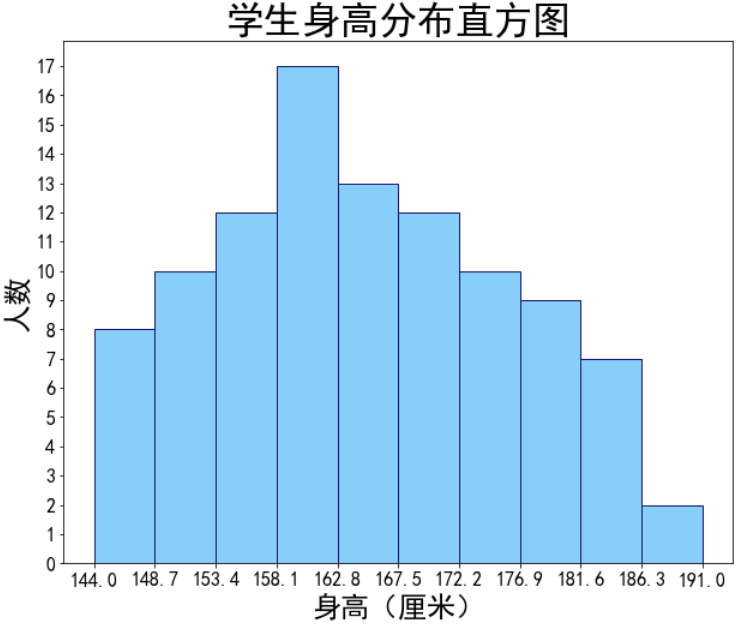
\includegraphics[width=0.5\textwidth]{直方图1.png}
\end{figure}

直方图比分位数表格更直观、更容易理解。我们可以直接看出,学生身高在$[158.1, \,\, 162.8)$区间最为集中,共有$17$人的身高落在这个区间里;
在$[186.3, \,\, 191]$区间最为稀疏,只有$2$人的身高落在这个区间里。

比直方图更简单的描述方法是\textbf{平均数和方差}。平均数是所有样本值之和除以样本数的商。如果所有样本值相差不多,
那么平均数可以告诉我们样本值大致分布在哪里。
比如,算得$100$个学生的身高值之和为$16426.5$厘米,则他们身高的平均值为$164.265$厘米。如果所有学生身高相差不多,
就可以说他们的身高大致是$164$厘米。

当然,我们从直方图可以看出,学生的身高差距并非“不多”。
因此,我们引入\textbf{方差}的概念,描述样本值的集中程度。
方差和平均数一起,可以粗略呈现样本分布的情况。样本的方差定义为样本值与均值之差的平方的均值。给定$N$个样本值:
$x_1, x_2, \cdots, x_N$,记它们的均值为$u$,方差为$v$,则:
$$ v = \frac{1}{N}\sum_{i=1}^N \left(x_i - u\right)^2.$$
由于$u = \frac{1}{N}\sum_{i=1}^N x_i$,可以推出:
$$v = \frac{1}{N}\sum_{i=1}^N x_i^2 - u^2.$$
比如,$1,2,3,4,5$的平均数为:
$$ \frac{1+2+3+4+5}{5} = 3,$$
方差为:
$$ \frac{(1 - 3)^2 + (2 - 3)^2 + (3 - 3)^2 + (4 - 3)^2 + (5 - 3)^2}{5} = 2.$$

方差的概念在单批样本中比较难理解,但如果用于比较两批样本,就容易理解了。举例来说,考察某地连续两年的日均降雨量,
绘制直方图:
\begin{figure}[H] %this figure will be at the right
    \vspace{10pt}
    \centering
    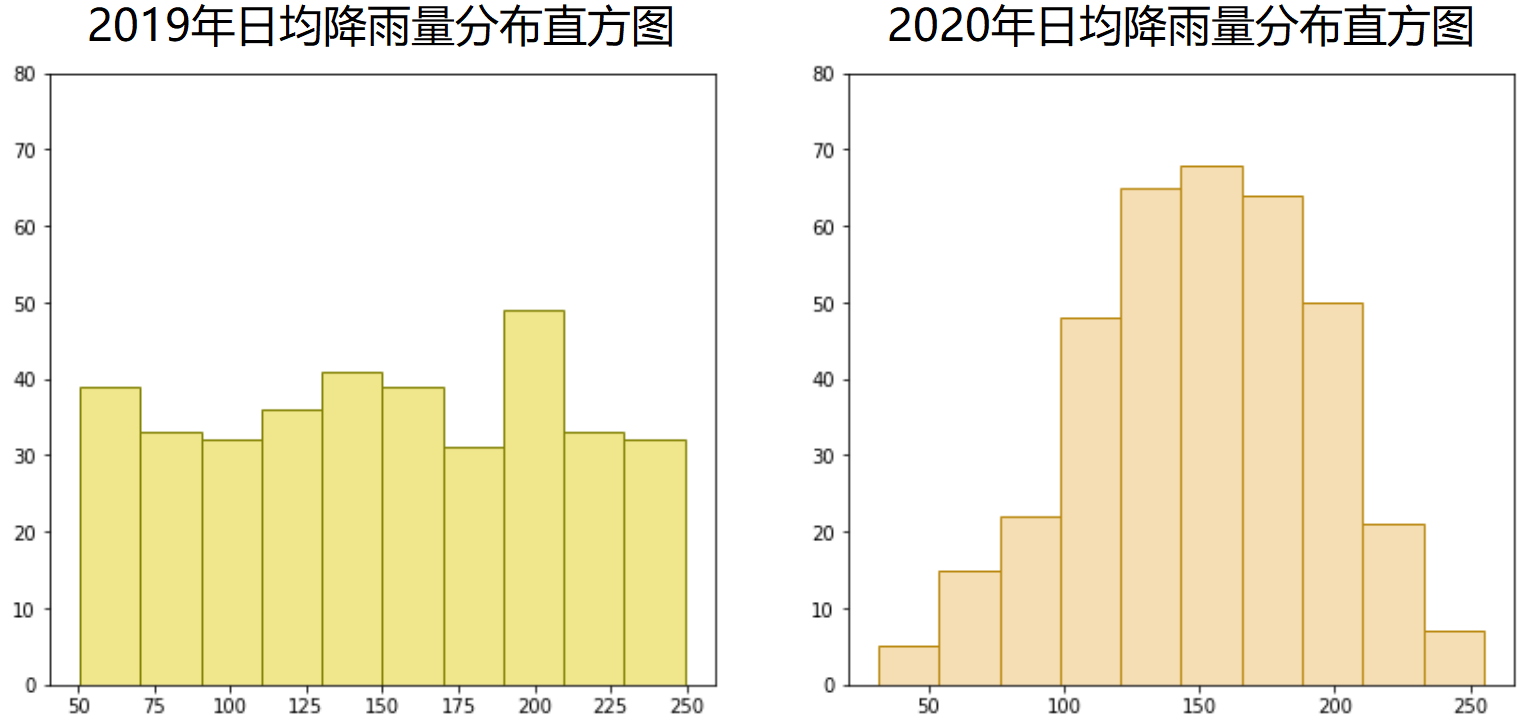
\includegraphics[width=0.96\textwidth]{直方图方差1.png}
\end{figure}
可以看出,虽然两年平均降水量差不多,但相比$2019$年,$2020$年的日均降雨量分布较为集中。
计算得到的方差也说明这一点:$2019$年日均降雨量的方差为$3147.87$,而$2020$年日均降雨量的方差只有$1872.21$。


\begin{sk}
    \mbox{} \\
    \indent 1. 能否把分位数表格的信息用图表形式展示?\\
    \indent 2. 绘制直方图时,是否有别的方式划分区间?\\
    \indent 3. 分位数表格和直方图有什么联系?\\
    \indent 4. 直方图划分的区间个数是否越多越好?你认为应该如何确定划分的区间数?\\
    \indent 5. 除了方差,你还能想到什么方法来描述数据的集中程度?它们和方差相比有什么好处?
\end{sk}

\begin{xt}
    \mbox{} \\
    \indent 1. 写出右分位数的自然定义。\\
    \indent 2. 写出顺右分位数的定义。
\end{xt}

\section{数据的结构}
上一节中我们描述、分析数据的时候,并未考虑数据本身的结构。什么是数据的结构?
数据结构是不同数据样本之间因数据自身含义产生的联系的总和。
用适合的方式展现数据的结构,有助于我们理解数据包含的信息,描述并分析数据。

一种常见的数据结构是时空结构:不同的数据样本代表了不同时间不同地点的信息。
用合适的方式展现这种时空结构,对我们研究相关事物大有帮助。

举例来说,下表中有我国部分地区某日的日均气温数据。
% 各地气温
\begin{center}
    \begin{tabular}{ p{4em}<{\centering} !{\color{white} \vrule width 2pt} p{4.6em}<{\centering} !{\color{white} \vrule width 2pt} p{4.8em}<{\centering} !{\color{white} \vrule width 2pt} p{4.8em}<{\centering} !{\color{white} \vrule width 2pt} p{4.6em}<{\centering} }
        \rowcolor{gd} \textbf{地区编号} & \textbf{日期} & \textbf{经度} & \textbf{纬度} & \textbf{气温(°C)} \\ [0.5ex] 
        \noalign{{\color{white}\hrule height 2pt}} % \hline\hline
        \rowcolor{gl} $391027$ & $2021–09–01$ & $110.530128$ & $34.754986$ & $15.9$  \\  
        \noalign{{\color{white}\hrule height 2pt}}% \hline
        \rowcolor{gd} $391028$ & $2021–09–01$ & $111.105681$ & $35.516971$ & $18.9$  \\  
        \noalign{{\color{white}\hrule height 2pt}}% \hline
        \rowcolor{gl} $391029$ & $2021–09–01$ & $111.183294$ & $34.207944$ & $19.3$  \\  
        \noalign{{\color{white}\hrule height 2pt}}% \hline
        \rowcolor{gd} $\vdots$ & $\vdots$ & $\vdots$ & $\vdots$ & $\vdots$ \\  
    \end{tabular}
\end{center}

从列表中难以看出数据之间的联系。
我们可以把相关的数据展示在对应的地理位置上,形成下图:
% 热力图
\begin{figure}[H] %this figure will be at the right
    \vspace{8pt}
    \centering
    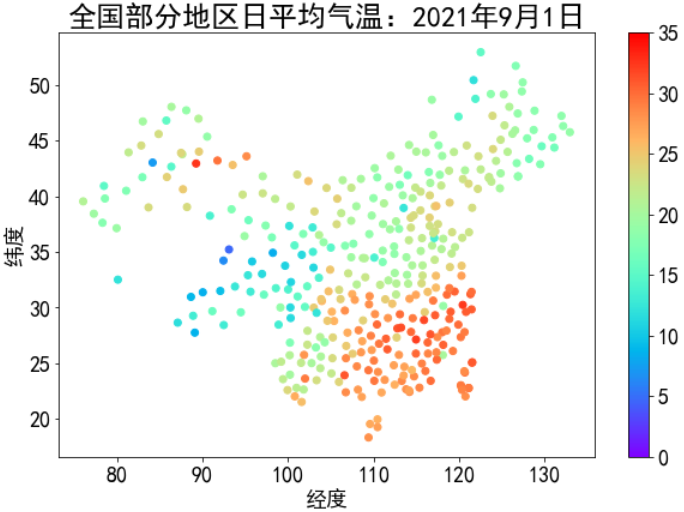
\includegraphics[width=0.5\textwidth]{全国日均气温1.png}
\end{figure}

这种图叫\textbf{热力图},能直观表现各地气温之间的关系。

以上是空间地域结构的展示。再来看时间结构的展示。下表是$2005$年至$2010$年成都市月均气温和降水量数据。
% 月降水量和气压数据
\begin{center}
    \begin{tabular}{ p{4.6em}<{\centering} !{\color{white} \vrule width 2pt} p{7em}<{\centering} !{\color{white} \vrule width 2pt} p{7em}<{\centering} }
        \rowcolor{gd} \textbf{月份} & \textbf{气温(°C)} & \textbf{降水量(毫米)} \\ [0.5ex] 
        \noalign{{\color{white}\hrule height 2pt}} % \hline\hline
        \rowcolor{gl} $2005–03$ & $14.3$ & $69.3$ \\ 
        \noalign{{\color{white}\hrule height 2pt}}% \hline
        \rowcolor{gd} $2005–01$ & $\,\,\,7.9$ & $10.3$ \\  
        \noalign{{\color{white}\hrule height 2pt}}% \hline
        \rowcolor{gl} $2005–02$ & $10.0$ & $27.5$ \\ 
        \noalign{{\color{white}\hrule height 2pt}}% \hline
        \rowcolor{gd} $\vdots$ & $\vdots$ & $\vdots$ \\  
        \noalign{{\color{white}\hrule height 2pt}}% \hline
        \rowcolor{gl} $2010–12$ & $\,\,\,9.5$ & $35.5$ \\ 
    \end{tabular}
\end{center}

从列表中难以看出数据之间的联系。可以把数据按时间先后顺序排列,这样得到的数据称为\textbf{时间序列}。
以$x$轴表示时间,以$y$轴表示气温和降水量,按照时间先后顺序,把每个月的气温和降水量对应的点用线段连起来,
就形成下图:
% 时间序列
\begin{figure}[H] %this figure will be at the right
    \vspace{8pt}
    \centering
    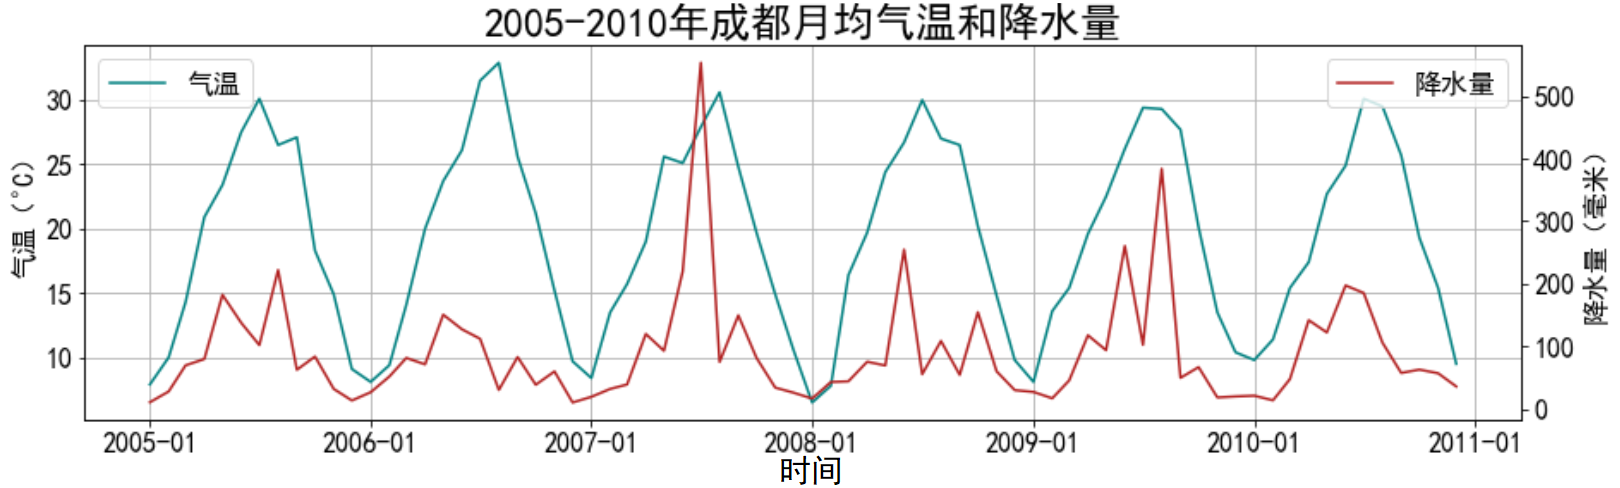
\includegraphics[width=0.9\textwidth]{时间序列1.png}
\end{figure}
从图中,我们容易看出当地降水量和气温数据随时间变化的方式。这种呈现数据的方式称为\textbf{折线图}。

另一个例子涉及更复杂的关系。下表中有某工厂完成一个项目所需的任务、
各项任务的前置任务(完成前置任务才能开始本任务)和预计用时: 
% 事务列表
\begin{center}
    \begin{tabular}{ p{4em}<{\centering} !{\color{white} \vrule width 2pt} p{4em}<{\centering} !{\color{white} \vrule width 2pt} p{4em}<{\centering} }
        \rowcolor{gd} \textbf{任务编号} & \textbf{预计用时} & \textbf{前置任务}  \\ [0.5ex] 
        \noalign{{\color{white}\hrule height 2pt}} % \hline\hline
        \rowcolor{gl} $1$ & $7$ & $3, \,\, 4$ \\  
        \noalign{{\color{white}\hrule height 2pt}}% \hline
        \rowcolor{gd} $2$ & $8$ & $1$  \\ 
        \noalign{{\color{white}\hrule height 2pt}}% \hline
        \rowcolor{gl} $3$ & $4$ & -  \\  
        \noalign{{\color{white}\hrule height 2pt}}% \hline
        \rowcolor{gd} $4$ & $5$ & -  \\ 
        \noalign{{\color{white}\hrule height 2pt}}% \hline
        \rowcolor{gd} $\vdots$ & $\vdots$ & $\vdots$ \\  
    \end{tabular}
\end{center}
从列表中难以判断应该如何组织工作。我们可以把各项任务的关系用箭头连接起来,用图表来表示:
% 事务关系有向图
\begin{figure}[H] %this figure will be at the right
    \vspace{8pt}
    \centering
    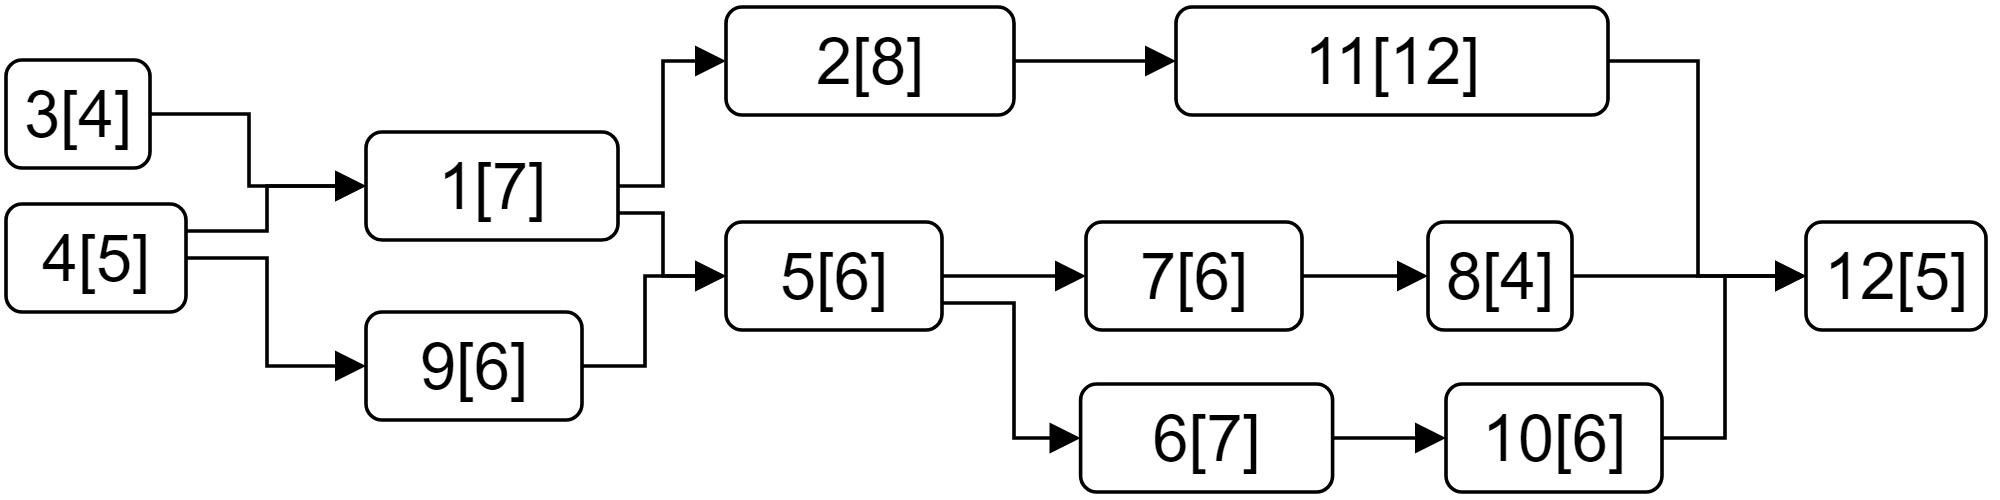
\includegraphics[width=0.8\textwidth]{流程图1.png}
\end{figure}

这个展示数据的方法称为\textbf{流程图}。图中将任务用圆角方块表示,
方块长度和任务预计用时成正比。方块中标明了任务编号和预计用时(方括号内)。
用箭头把每个任务指向它的后继任务(必须完成本任务才能开始后继任务)。
据此,我们就能更好地理解完成任务的必要次序,更合理地安排工作。

\chapter{数据和概率}
之前,我们学习了用概率来讨论不确定的事件。如何判断某件事情将来会不会发生?
我们需要通过已有的知识和经验来分析。数据就是我们对已有知识和经验的总结、提炼。
通过分析数据,我们可以讨论不确定的事件发生的概率。

\section{实验和样本}
为了研究我们关心的问题中某些随机事件发生的规律,我们会特意设计\textbf{实验},布置相关条件,
并观察发生的事件,记录结果。每次实验,我们得到的结果就是一个数据样本。
比如,为了研究投骰子各面朝上的规律,我们设定骰子的大小、材料和形制,设计投掷的高度,
并观察投掷结果。这就是一个实验。

实际中,很多问题并不是人类有能力设计、布置必要条件的,但我们仍然关心其中随机事件发生的规律,
比如台风、地震、火山爆发等等。因此,我们假设大自然设计了相关的实验,框定一些假设条件,
并观察发生的事件,记录结果。我们称之为广义的实验。比如,为了研究我们所在地区的降雨情况,
我们观察每天是否降雨,记录降雨量,就是一次广义的实验。为了研究方便,
我们会假设记录地点代表了所在地区(比如全市)的平均降雨情况,
或者设定每天降雨量为早上$8$点到次日早上$8$点之间的记录量等等,但我们无法完全控制实验的条件。

一次大实验可以包含几个小实验。比如,我们可以把连续记录一周的日降雨量称为一次实验,
也可以把每天的记录称为一次实验。为了好说话,我们会区分\textbf{单一实验}和\textbf{复合实验}。如何区分,
取决于我们关心的问题的性质和我们的研究方法。
比如,体检中,我们可以把测量每个学生身高、体重、血压和肺活量合称为一个单一实验,
这样,测量$100$个学生就是复合实验。如果我们关心的是这些学生的整体状况,
我们可以认为这是$1$次复合实验,其中每个学生的测量称为单一实验。
如果我们关心的是某个学生的状况,那么我们可以重复测量这个学生$100$次,称为复合实验,其中每次测量称为单一实验。

实验中,我们观察某些事件发生的情况,把我们关心的部分用数据记录下来,这样就得到一个数据样本。
这样记录的叫做实验的\textbf{终态}或\textbf{结果}。

\section{随机变量}

一般来说,我们把实验的每个结果关联到某个方便理解的数值,作为数据记录。
这样的映射,称为\textbf{随机映射}或\textbf{随机变量}。比如,设计抛掷硬币的实验,每次投掷如果正面向上,
就规定结果是$1$,否则规定结果是$0$。那么我们可以把投掷结果用随机变量表示:
\begin{align}
    h \,\,\, : \,\,\, \{\mbox{正面}, \mbox{反面}\} &\rightarrow \{0,\,\, 1\} \notag \\
    h(\mbox{正面}) &= 1 \notag \\
    h(\mbox{反面}) &= 0 \notag 
\end{align}
随机变量$h$把终态“正面”映射到$1$,把终态“反面”映射到$0$。

又比如,为了研究投骰子各面朝上的规律,我们设计投掷骰子的实验,
每次投掷的结果是朝上的数字,我们约定,每次投掷骰子,得到的收益是这个数值的$10$倍。
如果数字$2$朝上,就获得$20$元;数字$5$朝上,就获得$50$元,等等。
则我们可以把每次投掷骰子的收益用随机变量表示:
\begin{align}
f \,\,\, : \,\,\, \{1,2,3,4,5,6\} &\rightarrow \{10,20,30,40,50,60\} \notag \\
 i &\rightarrow 10\times i \notag 
\end{align}
随机变量$f$把终态$1$映射到$10$,把终态$2$映射到$20$,把终态$3$映射到$30$,等等。

一般来说,设试验的终集为$S$,如果某个映射把终集里的每个终态映射到另一个集合$X$里,
就说这个映射是$S$上的$X$–随机映射或随机变量。如果集合$X$是有限集合或有理数集的子集,
就说随机映射是\textbf{离散}的;如果集合$X$是实数集或区间,就说随机映射是\textbf{连续}的。

我们把随机变量背后随机事件的概率分布,称为\textbf{随机变量的分布}或随机变量遵循的分布。
可以看出,随机变量的性质与其分布有关。
随机变量的分布如何具体影响随机变量呢?我们来看两个例子。
\begin{ex}
    考虑这样的映射$\mathbb{E}$:它将离散随机变量$f$映射为
    $$ \mathbb{E}(f) = \sum_{s\in S} f(s) \mathbb{P}(\{s\}).$$
    这个映射称为随机变量的期望。比如,对以上掷骰子试验的随机变量$f$,它的期望为:
    $$ \mathbb{E}(f) = \sum_{i=1}^6 10\cdot i \mathbb{P}(\{i\}).$$
    如果投骰子的分布是均匀分布,那么对任何$i$​,$\mathbb{P}(\{i\})$​总是$\frac{1}{6}$​,于是:
    $$ \mathbb{E}(f) = \sum_{i=1}^6 \frac{10\cdot i}{6} = 35. $$
    如果$1$朝上的概率是$50\%$,其他数字朝上的概率都是$10\%$​,那么:
    $$ \mathbb{E}(f) = 10\cdot 1\cdot 50\% + \sum_{i=2}^6 \frac{10\cdot i}{10} = 25. $$
    随机变量分布改变,它的期望也可能改变。
\end{ex}
\begin{ex}
    考虑这样的映射$\mathrm{Var}$:它将离散随机变量$f$映射为

    $$ \mathrm{Var}(f) = \sum_{s\in S} \left(f(s) - \mathbb{E}(f)\right)^2 \mathbb{P}(\{s\}).$$
    这个映射称为随机变量的变差。比如,对以上掷骰子试验的随机变量$f$,它的期望为:
    $$ \mathrm{Var}(f) = \sum_{i=1}^6 \left(10i - \mathbb{E}(f)\right)^2 \mathbb{P}(\{i\}).$$
    如果投骰子的分布是均匀分布,那么对任何$i$,$\mathbb{P}(\{i\})$总是$\frac{1}{6}$,于是$\mathbb{E}(f) = 35$,因此:
    $$\mathrm{Var}(f) = \sum_{i=1}^6 \frac{\left(10i - 35\right)^2}{6} = \frac{875}{3} \approx 291.67$$    
    如果$1$朝上的概率是$50\%$,其他数字朝上的概率都是$10\%$,那么$\mathbb{E}(f) = 25$,因此:    
    $$ \mathbb{E}(f) = (10\cdot 1 - 25)^2\cdot 50\% + \sum_{i=2}^6 \frac{(10\cdot i - 25)^2}{10} = 325 $$
    随机变量分布改变,它的变差也可能改变。
\end{ex}

另一种表示随机变量分布的方法,是\textbf{概率密度函数}。
概率密度函数从随机变量的值出发描述它遵循的分布,把$X$中元素值映射到“随机变量等于该值”这一事件的概率。
比如,投掷骰子的随机变量$f$的分布,可以用以下的概率密度函数表示:
\begin{align}
p_f \,\,\, : \,\,\,  \{10,20,30,40,50,60\} &\rightarrow \qquad\qquad\qquad [0, \,\, 1] \notag \\
  x\qquad\qquad &\mapsto \,\, \mathbb{P}(\{s \in \{1,2,3,4,5,6\} \,|\, f(s) = x\}) \notag 
\end{align}

概率分布不同,随机变量$f$的概率密度函数也不同。
例如,投骰子的分布是均匀分布时,$p_f(10) = \frac{1}{6}$;如果$1$朝上的概率是$50\%$,
那么$p_f(10) = \frac{1}{2}$。

使用概率密度函数,也可以表示随机变量的期望和变差。对$X$中每个元素$x$,考虑使$f(s) = x$的$s$。我们发现:
\begin{align}
    \sum_{f(s) = x} f(s) \mathbb{P}(\{s\}) &= \sum_{f(s) = x} x \mathbb{P}(\{s\}) \notag \\
    &= x \sum_{f(s) = x} \mathbb{P}(\{s\}) \notag \\
    &= x \mathbb{P}(\{s \in S \,|\, f(s) = x\}) \notag \\
    &= x p_f(x) \notag  
\end{align}
因此,随机变量$f$的期望
$$ \mathbb{E}(f) = \sum_{s\in S} f(s) \mathbb{P}(\{s\}) = \sum_{x \in X} x p_f(x). $$
这是因为当$x$遍历$X$时,使$f(s) = x$的$s$也遍历了$S$,没有重复也没有遗漏。

同理可以推出,随机变量$f$的变差可以写成:
$$ \mathrm{Var}(f)  = \sum_{x\in X} \left(x - \mathbb{E}(f)\right)^2 p_f(x).$$ 

如何理解随机变量的期望和变差呢?

首先来看期望。随机变量的期望可以看作一种对实验结果预期的描述。举例来说,考虑以上掷硬币的实验的随机变量$h$。
假设硬币正面朝上的概率是$p$,那么$h$的期望是:
$$ \mathbb{E}(h) = 1\cdot p + 0\cdot (1 - p) = p. $$
于是,期望越大,表示$p$越大,说明掷硬币越可能正面朝上;反之说明掷硬币更可能反面朝上。又比如,考虑以上掷骰子的实验的随机变量$f$。
假设各面朝上的概率分别是$p_1, p_2, \cdots , p_6$,那么$f$的期望是:
$$ \mathbb{E}(h) = 10p_1 + 20p_2 + \cdots + 60p_6. $$
如果$p_1$接近于$1$,其它概率接近$0$,那么$\mathbb{E}(h)$接近于$10$,即预期收益和$1$点向上的收益相近。
如果$p_1$接近于$5$,其它概率接近$0$,那么$\mathbb{E}(h)$接近于$50$,即预期收益和$5$点向上的收益相近。

一般来说,随机变量的期望是一种方便的描述预期结果的方法。概率越大的终态,对期望的影响越大,反之亦然。

再来看变差的作用。在投骰子的例子里,考虑以下两种概率分布:
\begin{enumerate}
    \item $p_1 = p_6 = 40\%$,$p_2 = p_3 = p_4 = p_5 = 5\%$。
    \item $p_3 = p_4 = 40\%$,$p_1 = p_2 = p_5 = p_6 = 5\%$。
\end{enumerate}
两种情况下,随机变量的期望相同,都是$35$,但显然这两种分布有很大区别。而变差可以描述这两种分布的区别。
计算两种情况的变差,分别得到$525$和$85$。可以观察到,期望相同的情况下,分布的变差越大,结果远离期望值的概率越大,
变差越小,结果远离期望值的概率越小。通过期望和变差,我们可以对概率分布有粗略的了解。

\begin{sk}
    \mbox{} \\
    \indent 1. 概率映射和随机变量有什么不同? \\
    \indent 2. 比较随机变量的期望和样本数据的平均数。它们有什么相似之处?有什么不同?\\
    \indent 3. 比较随机变量的变差和样本数据的方差。它们有什么相似之处?有什么不同?\\
    \indent 4. 随机变量的分布改变,它的期望一定改变吗?\\
    \indent 5. 随机变量的分布改变,它的变差一定改变吗? \\
    \indent 6. 随机变量的期望和变差的不同写法有哪些要注意的地方?你觉得每种写法好在哪里?   
\end{sk}

\begin{xt}
    \mbox{} \\
    \indent 1. 小李投掷一枚$1$元硬币,约定正面向上则小王给小李$10$元钱,否则小王给小李$1$元钱。\\
    \indent 1.1. 假设硬币正面向上的概率是$47\%$,试将小王给小李的钱数用相关的随机变量表示。\\
    \indent 1.2. 该随机变量的分布是什么分布?    \\
    \indent 1.3. 写出该随机变量的概率密度函数。\\
    \indent 1.4. 写出该随机变量的期望和变差。\\
    \indent 2. 投掷一枚骰子,假设$1$点向上和$5$点向上的概率分别是$40\%$,其余点数向上的概率是$5\%$,
    如果以点数的$3$倍为随机变量,求它的期望和变差。\\
    \indent 3. $X$是$\mathbb{Q}$的子集。证明$S$上的$X$–随机变量$f$的变差也可以写成:
    $$ \mathrm{Var}(f)  = \mathbb{E}(f^2) - \mathbb{E}(f)^2.$$  
    \indent \hspace{1em}  其中$f^2$表示把每个终态$s$映射到$f(s)^2$的随机变量。
\end{xt}

\section{条件概率和独立事件}
讨论随机事件,总要知道前提条件。只有明确了前提条件,才能讨论事件的概率。
为了研究不同的前提条件对事件的影响,我们引入\textbf{条件概率}的概念。

仍以“明天杭州是否下雨”为例。我们讨论台风“凤凰”动向对下雨概率的影响,可以说:
“如果台风靠近,那么下雨的概率有$90\%$”、“如果台风转向,那么不下雨的概率为$40\%$”。
这里我们把台风靠近与否作为明天杭州下雨的前提条件。以上两句话可以记作:
$$ \mathbb{P} (\{\mbox{下雨}\} \, | \, \{\mbox{台风靠近}\}) = 0.9, \quad \mathbb{P} (\{\mbox{不下雨}\} \, | \, \{\mbox{台风转向}\}) = 0.4$$

从中可以推出,如果台风靠近,那么不下雨的概率是$10\%$;如果台风转向,那么下雨的概率是$60\%$。
我们可以把这些概率用表格的形式表示:

% 条件概率表格
\begin{center}
    \begin{tabular}{ p{6.4em}<{\centering} !{\color{white} \vrule width 2pt} p{6.4em}<{\centering} !{\color{white} \vrule width 2pt} p{6.4em}<{\centering} }
        \rowcolor{gd} \textbf{条件} & 下雨 & 不下雨 \\ [0.5ex] 
        \noalign{{\color{white}\hrule height 2pt}} % \hline\hline
        \rowcolor{gl} 台风靠近 & $90\%$ & $10\%$ \\ 
        \noalign{{\color{white}\hrule height 2pt}}% \hline
        \rowcolor{gl} 台风转向 &$60\%$ & $40\%$ \\   
    \end{tabular}
\end{center}

可以看到,台风靠近与否,会影响明天杭州下雨的概率。如果把台风“凤凰”的动向视为一个实验,
把“明天杭州是否下雨”视为另一个实验,我们也可以说,前一个实验影响了后一个实验的结果。

条件概率和概率之间的联系是怎样的呢?观察下图,可以发现,在假定事件$B$发生的条件下,发生事件$A$的条件概率,就是$A,B$同时发生的概率,除以事件$B$的概率。用公式表达出来,就是:
$$
\mathbb{P}(A \, | \, B) = \frac{\mathbb{P}(A \cap B)}{\mathbb{P}(B)}
$$
我们称$\mathbb{P}(A \, | \, B)$为“$B$时$A$的概率”。要注意的是,这个公式没有考虑$\mathbb{P}(B) = 0$的情况。如果$B$的概率是$0$,那么讨论$B$发生时$A$有多大可能发生没有意义。这时候我们不定义条件概率$\mathbb{P}(A \, | \, B)$。

从映射的角度来看,从事件$A$到$B$时$A$的概率形成这样一个映射:

$$ A \mapsto \mathbb{P}(A \, | \, B)$$

可以验证,这个映射也是一个概率映射,叫作关于$B$的条件概率映射。
我们一般把这个映射记为$\mathbb{P}_B$或$\mathbb{P}(\cdot\,|\,B)$(其中的$\cdot$表示自变量的位置)。

再来看另一个例子:有面值为$5$角和$1$元的硬币各一枚。首先抛出$1$元硬币,再抛出$5$角硬币,
把$1$元硬币抛掷结果看作$5$角硬币抛掷结果的前提条件。假设$1$元硬币正面朝上时,
$5$角硬币正面朝上的概率是$60\%$,反面朝上的概率是$40\%$;$1$元硬币反面朝上时,
$5$角硬币正面朝上的概率是$60\%$,反面朝上的概率是$40\%$。可以用表格表示条件概率:

\begin{center}
    \begin{tabular}{ p{6.4em}<{\centering} !{\color{white} \vrule width 2pt} p{6.4em}<{\centering} !{\color{white} \vrule width 2pt} p{6.4em}<{\centering} }
        \rowcolor{gd} \textbf{条件} & $5$角正面朝上 & $5$角反面朝上 \\ [0.5ex] 
        \noalign{{\color{white}\hrule height 2pt}} % \hline\hline
        \rowcolor{gl} $1$元正面朝上 & $60\%$ & $40\%$ \\  
        \noalign{{\color{white}\hrule height 2pt}}% \hline
        \rowcolor{gl} $1$元反面朝上 &$60\%$ & $40\%$ \\  
    \end{tabular}
\end{center}

可以看到,$1$元硬币抛掷结果,不影响$5$角硬币各面朝上的概率。“抛掷$1$元硬币”这个实验的结果,
不影响“抛掷$5$角硬币”实验的结果。

如果两个实验的结果互不影响,就说两者\textbf{相互独立}。一般来说,当我们讨论实验中发生的事件时,也说两个事件相互独立。

如果事件$A,B$相互独立,那么$B$时$A$的概率应该和$A$的概率一样。也就是说,
$$\mathbb{P}(A) = \mathbb{P}(A \, | \, B) = \frac{\mathbb{P}(A \cap B)}{\mathbb{P}(B)}.$$
即:
$$\mathbb{P}(A \cap B) = \mathbb{P}(A) \cdot \mathbb{P}(B).$$
同样地,
$$\mathbb{P}(B \, | \, A) = \frac{\mathbb{P}(A \cap B)}{\mathbb{P}(A)} = \frac{\mathbb{P}(A) \cdot \mathbb{P}(B)}{\mathbb{P}(A)} = \mathbb{P}(B).$$
多个事件之间也可能相互独立。给定$n$个事件$A_1, A_2, \cdots, A_n$,如果它们的交集的概率等于各自概率的乘积:
$$\mathbb{P}(A_1\cap A_2\cap \cdots \cap A_n) = \mathbb{P}(A_1) \mathbb{P}(A_2) \cdots \mathbb{P}(A_n),$$
就说它们相互独立。

\begin{xt}
    \mbox{} \\
    \indent 1. 证明:$\mathbb{P}(A \, | \, B) + \mathbb{P}(A^c \, | \, B) = 1$。 \\
    \indent 2. 证明:如果事件$A_1,A_2$互斥,那么$\mathbb{P}(A_1 \cup A_2\, | \, B) = \mathbb{P}(A_1 \, | \, B) + \mathbb{P}(A_2 \, | \, B)$。 \\
    \indent 3. 证明:$\mathbb{P}(A) = \mathbb{P}(A \, | \, B) \mathbb{P}(B) + \mathbb{P}(A \, | \, B^c) \mathbb{P}(B^c)$。 \\
    \indent 4. 证明全概率公式:如果$B_1, B_2, \cdots, B_k$两两互斥,且并集为全集,那么$\mathbb{P}(A) = \mathbb{P}(A \, | \, B_1) \mathbb{P}(B_1) + \mathbb{P}(A \, | \, B_2) \mathbb{P}(B_2) + \cdots + \mathbb{P}(A \, | \, B_k) \mathbb{P}(B_k)$。 \\
    \indent 5. 证明:$\mathbb{P}(B \, | \, A) = \frac{\mathbb{P}(A \, | \, B) \mathbb{P}(B)}{\mathbb{P}(A \, | \, B) \mathbb{P}(B) + \mathbb{P}(A \, | \, B^c) \mathbb{P}(B^c)}$。 \\
    \indent 6. 证明反条件概率公式:如果$B_1, B_2, \cdots, B_k$两两互斥,且并集为全集,那么$\forall i\in[1..k], \,\,\, \mathbb{P}(B_i \, | \, A) = \frac{\mathbb{P}(A \, | \, B_i) \mathbb{P}(B_i)}{\mathbb{P}(A \, | \, B_1) \mathbb{P}(B_1) + \mathbb{P}(A \, | \, B_2) \mathbb{P}(B_2) + \cdots + \mathbb{P}(A \, | \, B_k) \mathbb{P}(B_k)}$。 \\
    \indent 7. 抛掷两枚硬币,假设两次抛掷互不影响,每枚硬币抛出正反的概率相同。定义$A$为事件“第一枚抛出正面”,$B$为“第二枚抛出正面”,$C$为“两枚硬币抛掷结果相同”。 \\
    \indent 7.1. 求$A$、$B$、$C$的概率。\\
    \indent 7.2. 求$A\cap B$、$A\cap C$、$B \cap C$的概率。\\
    \indent 7.3. $A,B$是否相互独立?$B,C$是否相互独立?$A.C$是否相互独立?$A,B,C$是否相互独立?
\end{xt}

\section{大数定律}

我们做这样一个复合实验:取同一个骰子,投掷$100$次,每次为一次单一实验。
记录每次朝上的点数作,按其$10$倍给出收益,作为结果。
我们假定投掷结果是两两相互独立的事件,即前面投掷的结果不影响后面投掷的结果,反之亦然。
我们还假定每次投掷的实验条件都是相同的,忽略投掷姿势、高度等差别。
在这样的假定下,我们说,这$100$次投掷是$100$次\textbf{独立重复实验}。

独立重复实验是寻找随机事件规律的常用手段。比如,我们对投掷这枚骰子时各面朝上的概率一无所知,
只有一份$100$次独立重复的投掷实验的结果。这时,如果要讨论下一次投掷的结果,我们如何给出合理的预测呢?

对于这$100$次独立重复实验,我们可以定义随机变量$f_1,f_2,\cdots , f_{100}$,来表示每次实验的结果。
由于我们假设这些随机变量相互独立,而且遵循相同的分布,
我们说这$100$个随机变量是\textbf{独立同分布}的。

对于独立同分布的一组随机变量,我们有以下的定理:
\begin{tm}\textbf{大数定律}
    设一组随机变量$f_1, f_2, \cdots, f_{N}$相互独立,且都遵循同一个分布,
    它们的期望同为实数$u$,那么$N$越大,它们的平均数:
    $$\frac{1}{N}\left(f_1 + f_2 + \cdots + f_{N}\right)$$
    就几乎总会越来越接近$u$。
\end{tm}

大数定律是长久以来人们观察得出的一系列结论的总称,表示事情重复发生的数量足够多的时候,就会呈现一定的规律。
后来人们找到了合适的数学语言来描述这些定律,发现大数定律是一类数学定理。
大数定律的证明较为复杂,这里我们不作证明,只给出其中一个结论。

运用大数定律,我们可以为独立重复实验的结果给出什么结论呢?

大数定律建立了沟通实验结果平均数和随机变量期望的桥梁。已知独立重复实验的结果,那么对结果求平均数,就能估计出随机变量的期望。
而随机变量的期望,可以用来估计下一次实验的结果。

以上面投掷骰子的实验为例。设$100$次投掷实验的结果为$Y_1, Y_2, \cdots , Y_{100}$。它们分别是$100$个独立同分布的随机变量
$f_1, f_2, \cdots, f_{N}$的值。设下一次投掷实验的收益用独立同分布的随机变量$f$表示。根据大数定律,平均数
$$\overline{Y}_{100} = \frac{1}{100}(Y_1 + Y_2 + \cdots + Y_{100})$$
接近$f$的期望。因此,我们可以用$\overline{Y}_{100}$代表$f$的期望。比如,如果算得$\overline{Y}_{100} = 34.4$,
那么可以估计下一次投掷实验的预期收益是$34.4$。

再来看掷硬币实验,它对应的随机变量$h$将正面朝上映射到$1$,反面朝上映射到$0$。
已知正反面朝上的概率$p_{\text{正}}$和$p_{\text{反}}$,可以算得$h$的期望为:
$$ \mathbb{E}(h) = 1 \cdot p_{\text{正}} + 0 \cdot p_{\text{反}} = p_{\text{正}}.$$
所以,$h$的期望就是$p_{\text{正}}$。因此,如果投掷$1000$次硬币,其中$447$次正面朝上,
那么$h$的期望就接近于$\frac{447}{1000} = 0.447$。于是我们可以估计$p_{\text{正}} = 0.447$。
再掷一次硬币,正面朝上的概率是$44.7\%$。

从掷硬币实验的例子,还可以得到估计某事件概率的方法。如果能够作独立重复实验来观察事件$A$是否发生,那么我们把$n$次独立重复实验中
事件$A$的次数与试验次数$n$的比值称为该实验中$A$的频率,记为$q_A$。考虑把“事件$A$发生”映射到$1$,把“$A$不发生”映射到$0$的示性随机变量$f_A$,
那么频率$q_A$就是$n$个与$f_A$同分布的独立随机变量的平均数。根据大数定律,$n$很大的时候,$q_A$就接近$f_A$的期望,也就是$\mathbb{P}(A)$。
于是,通过记录多次实验中事件的频率,我们就可以估计事件发生的概率。

\begin{sk}
    \mbox{}\\
    \indent 1. 投掷一枚骰子,如果朝上的点数为$i$,则将$(2i-7)^2$作为结果。如果某骰子$1$向上的概率为$50\%$,其余点数朝上概率为$10\%$;
    另一枚骰子$6$向上的概率为$50\%$,其余点数朝上概率为$10\%$。设第一枚骰子的结果为随机变量$g_1$,第二枚为$g_2$,这两个随机变量是否同分布?\\
    \indent 2. 大数定律说明,独立重复实验次数足够多时,随机变量的期望可以用结果的平均数来估计。
    那么,独立重复实验次数足够多时,随机变量的变差能否用结果来估计呢?你有什么想法?
\end{sk}

\begin{xt}
    \mbox{}\\
    \indent 1. 将一枚硬币重复抛掷$200$次,其中$104$次正面向上。如何估计下一次抛掷时正面向上的概率?\\
    \indent 2. 将一枚骰子重复抛掷$1000$次,统计每次正面朝上的点数为结果。统计发现有$169$次$1$点、$142$次$2$点、$182$次$3$点、$163$次$4$点、$170$次$5$点、$174$次$6$点。\\
    \indent 2.1. 试估计下一次抛掷时得到$5$点的概率是多少?\\
    \indent 2.2. 试估计下一次抛掷时得到偶数点的概率是多少?\\
    \indent 2.3. 试估计下一次抛掷时点数不超过$3$的概率是多少?\\
    \indent 2.4. 试估计单次掷骰子结果的分布。
\end{xt}

% \chapter{运动和优化}
% \section{函数、图像和运动}
% \section{极值原理}
% \section{优化}

% \chapter{数学和社会}
% \section{随时代变化的数学}
% \section{数学和科学}
% \section{数学和现代化}

\end{document}